\documentclass[a4paper,12pt]{article}
\usepackage[margin=25mm]{geometry}
\usepackage{amsmath}
\usepackage{amsfonts}
\usepackage{amssymb}
\usepackage{setspace}
\usepackage{fancyhdr,natbib}
\pagenumbering{arabic}  
\pagestyle{plain}
\usepackage{multirow}
\usepackage{multicol}
\usepackage{booktabs}
\usepackage{hyperref}
\usepackage{subcaption}
\usepackage{placeins}
\usepackage{textgreek}
\usepackage{graphicx}
\pagenumbering{gobble}
\usepackage{libertinus}
\usepackage[scaled=0.83]{courier}
\usepackage[T1]{fontenc}
\usepackage[utf8]{inputenc}
\usepackage{latexsym}
\renewcommand{\UrlFont}{\ttfamily\small}
\usepackage{verbatim}
\usepackage{gb4e}


\title{Acquiring Pronoun Cases: \\Insights from Pronoun Case Errors}
\author{Xiaomeng Ma }
\date{}
\begin{document}
\pagestyle{plain}
\pagenumbering{arabic}
\maketitle
\section{Introduction}
English-speaking children make pronoun case errors from the age of two to four. Some common types of errors include: (1) using an accusative pronoun (e.g. \textit{me, him, us}) or a genitive pronoun (e.g. \textit{my, his, our}) as the subject of the sentence, see (\ref{1}) and (\ref{3}); (2) using a nominative pronoun (e.g. \textit{I, she, he}) or a genitive pronoun as the object in a sentence, see (\ref{2}) and (\ref{4}) and (3) using an accusative pronoun as the determiner, see (\ref{5}) and (\ref{6}). Researchers have categorized such errors as systematic, characteristic and frequent \citep[e.g.][]{huxley1970development, budwig1989linguistic, pelham2011input,fitzgerald2017case}.

\begin{exe}
\ex \label{01} non-nominative subject:
\begin{xlist}
\ex \label{1} {Where does \textit{him} go? - \textit{him} for \textit{he}, Becky at the age of 2;6\footnote{\href{https://childes.talkbank.org/browser/index.php?url=Eng-UK/Manchester/Becky/020619.cha}{Manchester/Becky/020619.cha}
}}
\ex \label{3} {\textit{My} get my car. - \textit{my} for \textit{I}, Nina at the age of 2;0\footnote{\href{https://childes.talkbank.org/browser/index.php?url=Eng-NA/Suppes/020003.cha}{Suppes/020003.cha}}}
\end{xlist}
\ex non-accusative object:
\begin{xlist}
\ex \label{2} {Mama put \textit{he} here. - \textit{he} for \textit{him}, Tow at the age of 1;9\footnote{\href{https://childes.talkbank.org/browser/index.php?url=Eng-NA/Post/Tow/010909.cha}{Post/Tow/010909.cha}}}
\ex \label{4} {Watch \textit{my} going round, Mum. - \textit{my} for \textit{me}, Gail at the age of 2;4\footnote{\href{https://childes.talkbank.org/browser/index.php?url=Eng-UK/Manchester/Gail/020421.cha}{Manchester/Gail/020421.cha}}}
\end{xlist}
\ex non-genitive determiner:
\begin{xlist}
\ex \label{5} He doesn't have \textit{them} claws. -\textit{them} for \textit{those/these} Roman at the age of 3;5\footnote{\href{https://childes.talkbank.org/browser/index.php?url=Eng-NA/Weist/Roman/030501.cha}{Weist/Roman/030501.cha}}
\ex \label{6} Um and that's \textit{me} name. - Fraser at the age of 3;0\footnote{\href{https://childes.talkbank.org/browser/index.php?url=Eng-UK/MPI-EVA-Manchester/Fraser/030025a.cha}{MPI-EVA-Manchester/Fraser/030025a.cha}}
\end{xlist}
\end{exe}

The most well-studied error is the non-nominative subject, where an accusative pronoun or a genitive pronoun is used in the subject position, as shown in (\ref{01}). Theoretically, the nominative case is licensed by the +\textsc{finite} feature on the IP. If the +\textsc{finite} is missing, the nominative case won't be checked. Therefore, the syntactic explanation linked this error with children's use of finite verbs \citep[e.g.][]{vainikka1993case,wexler1996, schutze1996subject}. Young children often go through a period in language development when they sometimes omit inflections on the verbs, producing non-finite forms such as `Then the horse \textit{jump}.' This developmental stage referred to by \cite{wexler1994,wexler1998,wexler2000} as the `Optional Infinitive Stage', where finiteness is optional in children's grammar, even though they already have the syntactic knowledge of tense and agreement. When the children produce a non-finite verb by omitting the inflections, the nominative case are not checked, leading to the non-nominative subject errors, such as `Then \textit{him/his} jump'. In the syntactic explanation, the non-nominative subject stems from children's problematic use of finite verbs and it is characteristic at Optional Infinitive Stage.

Although the syntactic explanation can account for many observed error patterns, not all the predictions are correct. According to the syntactic explanation, when a non-nominative subject is present, the verb in that sentence is unlikely to be a finite verb. \cite{pine2005testing} found that the data doesn't always support this prediction since it is not uncommon for children to produce non-nominative subjects with finite verbs. 

In addition, the syntactic explanation doesn't address the questions of individual variations, such as why different children make errors with different forms. For example, in example (\ref{1}), Becky replaced the nominative pronoun \textit{he} with its accusative form \textit{him}; whereas Nina replaced the nominative pronoun \textit{I} with the its genitive form \textit{my} in (\ref{3}). Meanwhile, \textit{my} was used as a substitute for the accusative pronoun \textit{me} by Gail in (\ref{4}).  \cite{rispoli1998} studied non-nominative use of pronoun \textit{I} and found that the majority of the children predominantly make `\textit{me}-for-\textit{I}' error and a minority predominantly make `\textit{my}-for-\textit{I}' error. He then found that the `\textit{me}-for-\textit{I}' is highly correlated with the correct use of `\textit{me}' in children's production. Thus, \cite{rispoli1998,rispoli1999,rispoli2005} treated pronoun case error as lexical retrieval error that is closely related with children's pronominal use. He proposed that for each pronoun, case, person, and number form a 3x3 paradigm. Young children have difficulties accessing all forms of pronouns in the paradigm, and thus make pronoun errors. 




In addition, parents' input also could play an important role in pronoun errors. \cite{pelham2011input} suggests that English children make more pronoun case errors than German children because English has more case-ambiguous pronouns (e.g. \textit{you}, \textit{it} and \textit{her}) than German. Parents' input also contains many ambiguous phrases like `Let \underline{\textit{me} do it}' or `help \underline{\textit{her} open it}' that could potentially confuse the children, that they would produce erroneous utterances such as `\underline{\textit{me} do it}' or `\underline{\textit{her} open it}' \citep{tomasello2000, kirjavainen2009can}.  




Apart from non-nominative subjects, children also substitute the accusative case for genitive case, as in (4) and substitute genitive case for an accusative case, as in (5). These errors have been generally overlooked by previous studies.
\begin{exe}
\ex [*]{Don't take \textit{me} bottle out. - \textit{me} for \textit{my}, Nina at the age of 2;1\footnote{\href{https://childes.talkbank.org/browser/index.php?url=Eng-NA/Suppes/020115.cha}{Suppes/020115.cha}}}
\ex [*]{Let \textit{my} try. - \textit{my} for \textit{me}, Carl at the age of 2;6\footnote{\href{https://childes.talkbank.org/browser/index.php?url=Eng-UK/Manchester/Carl/020619.cha}{Manchester/Carl/020619.cha}} }
\end{exe}
The existing explanations seem to fall short for these errors. The syntactic explanations treat the accusative case and the genitive case as two different default forms to the nominative case. If both cases are default, there is no incentive to substitute one default for the other as in (4) and (5). Moreover, parents' input never contain any segments that resemble the errors in (4) and (5): `take \textit{me} bottle' and `let \textit{my} try'. 

Moreover, after over 40 years of research, some basic properties of pronoun case errors are still unknown, such as the frequencies and distributions of the errors, at what age are those errors likely to occur, how prevalent are those errors among children, does the error disappear after the children reach a certain age or a certain MLU, etc. Few studies have reported comprehensive pronoun error counts or error rates; instead, most of the studies focused on a certain type of errors or pronouns in their analysis. A sizable longitudinal dataset is required to answer these questions. One common limitation for previous studies is their small sample size: \cite{schutze1996subject} included 3 children (Nina from \citep{suppes1974semantics}, Sarah from \citep{brown1973first} and Peter\citep{bloom1974imitation}); \cite{rispoli1998} collected data on 12 children from 1;0 to 3;0; \cite{kirjavainen2009can} conducted corpus analysis of 17 children in CHILDES (12 from Manchester corpus \cite{theakston2001}, Fraser and Eleanor from densed corpus \citep{rowland2006effect} and Abe from \cite{kuczaj1977acquisition}, Nina from \citep{suppes1974semantics} and Peter from \citep{bloom1974imitation}). Due to limited sample size, previous studies couldn't address these questions. 

This paper investigated pronoun case errors in children's production by conducting a comprehensive corpus analysis on all the available data of English-speaking children on \textsc{childes} \citep{macwhinney2014childes}. First, this paper reviewed some basic features of pronoun case errors, such as frequency and distribution, age range, correlation with age and MLU, etc. Second, this paper re-examined each existing explanations using all available CHILDES data. In the previous studies, researchers either collected their own data or used different corpora to test their hypotheses. It is necessary to evaluate different theories on the same set of data in order to control for collection bias or limitations of small sample size. 

Last, this paper will provide a hypothesis about how children acquire pronoun case in the first place. Cases are used to mark different relationship between arguments, which is a more abstract grammatical feature to learn compared to plural forms or tense marking. Yet young children are able to produce the correct form of a pronoun in different argument positions. It would be worthwhile to ask the question: how do children acquire this abstract feature at such a young age? This study is going to test two hypotheses of the acquisition of pronoun case. From a theoretical perspective, the children could derive different cases through argument structure. Nominative case and accusative case could be differentiated at the sentential level, such that the former is associated with the subject and the latter case is associated with the object. In addition, children could also acquire cases through statistical learning. Nominative case, accusative case and genitive case have different distributional patterns in speech, which difference could be utilized by children to acquire different cases. 

The paper is organized as follows: Section 2 presents a detailed description of pronoun case errors, including the basic properties metioned above; Section 3 - 5 replicates representative studies for existing explanations and evaluates that explanation; Section 6 demonstrates a computational model using distributional patterns to explain pronoun case acquisition.
\newpage
\section{The Basic Features of Pronoun Case Error}
\subsection{Corpora}
To avoid the limitation of small sample size and data selection bias, this study conducted a comprehensive corpus analysis of speech from monolingual English-speaking children from roughly ages two to four. That includes 46 children with longitudinal recordings in CHILDES. Table \ref{table:1} shows the summary of the corpus.

\begin{table}[h]
\footnotesize
\centering
\caption{Summary of Corpus Information} 
\label{table:1}
%\begin{adjustbox}
\begin{tabular}{l|l|l|l|l|l}
\toprule
\multicolumn{6}{c}{\textbf{North American Corpora}} &
\hline
\textbf{Corpora}  & \textbf{Child}  & \textbf{Age} &
\textbf{Corpora}  & \textbf{Child}  & \textbf{Age}\\
\hline
\cite{bloom1974imitation}  & Peter   & 1;9-3;2 & \cite{suppes1974semantics} &  Nina & 2;0-3;4
\\
\cite{braunwald1971mother}  & Laura   & 1;5-4;0 & \cite{kuczaj1978children} &  Abe & 2;5-4;0 \\
\multirow{}{}*{\cite{brown1973first}} & Adam & 2;3-4;0 & \cite{demetras1986working} & Trevor & 2;1-4;0\\
& Eve & 1;6-2;3 & \multirow{}{}*{\cite{Weist2009}} & Ben & 2;4-3;4 \\
& Sarah & 2;3-4;0 & &Emily & 2;6-3;4\\
\cite{demetras1989changes} & Jimmy & 2;2-2;10 & & Emma & 2;7-3;9\\
\cite{clark1978awareness} & Shem & 2;3-3;2 &  & Jilian & 2;1-2;10\\
\cite{sachs1983talking}& Naomi & 1;3-4;9 & & Matt & 2;5-5;0\\
\cite{macwhinney2014childes} & Ross & 1;4-5;0 & & Roman & 2;3-4;0\\
\multirow{}{}*{\cite{post1993language}}& She & 1;8-2;5 & \cite{Snow1990child} & Nathaniel & 3;1-3;3\\
&Tow&1;9-2;5&\cite{hayes1988vocabulary}&Geraldine&1;6-2;2\\
\hline
\hline
& \textbf{No.} & \textbf{Mean Age} & & \textbf{No.} & \textbf{Mean Age}\\
\cite{bates1991first}  & 11  & 2;4 &
\cite{bohannon1977children}  & 2 & 3;6\\
\cite{gleason1980acquisition}&19&4;8&\cite{snow1995shell}&79&3;11\\
\cite{snow1989imitativeness}&25&2;8&\cite{valian1991syntactic}&17&2;5\\
\cite{van1980effects}&19&3;9\\
\hline
\hline
\multicolumn{6}{c}{\textbf{UK Corpora}}&
\hline
\textbf{Corpora}  & \textbf{Child}  & \textbf{Age} &
\textbf{Corpora}  & \textbf{Child}  & \textbf{Age}\\
\hline
\multirow{}{}*{\cite{henry1995belfast}} & Barbara & 2;4-4;1 & \multirow{}{}*{\cite{theakston2001}} & Anne & 1;10-2;9\\
& Michelle & 2;4-4;4 & & Warren& 1;10-2;9 \\
& Courtney & 3;4-4;0 & &Aran & 1;11-2;10\\
 & Rachel & 2;5-3;2 & & Becky & 2;0-2;11\\
 & Conor & 3;8-4;5 &  & Carl & 1;8-2;8\\
& Stuart & 3;5-4;5 & & Dominic & 1;10-2;10\\
 & Johnny & 3;5-4;4 & & Gail & 1;11-2;11\\
 & David & 2;0-4;2 &  & Joel & 1;11-2;10\\
\cite{rowland2006effect} & Lara & 1;9-3;3&  & John &1;11-2;10 \\
\cite{maslen2004dense} & Thomas & 2;0-4;11 & & Liz& 1;11-2;10\\
\multirow{}{}*{\cite{lieven2009two}} &Eleanor &2;0-3;1 & & Nicole& 2;0-3;0 \\
&Fraser &2;0-3;0 & & Ruth& 1;11-2;11 \\
\hline
\hline
&\textbf{No.}&\textbf{Mean Age}& &\textbf{No.}&\textbf{Mean Age}\\
\cite{tommerdahl2013analyzing}&23&2;9&\cite{howe1981acquiring}&16&2;0\\
\hline
\bottomrule
\end{tabular}
%\end{adjustbox}
\end{table}

This study applied the \textsc{nltk} python package to automatically extract data from the annotated corpora in CHILDES. The data that has been collected from each child's file include their age, mlu, total number of children's words and parents' words, total number of children's sentences and parents' sentences, total number of each pronoun produced by the children and produced by the parents. 

\subsection{Finding Errors}
The annotated \texttt{.xml} files were used to search for the errors. CHILDES applies MOR and GRASP programs to annotate part-of-speech tags and dependency grammatical relations for all the transcripts. For English data, the automated annotation system has been reported to have high-level accuracies: the MOR program reaches 97\% of accuracy and the GRASP program has 95.8\% accuracy for identifying the subjects and 94.1\% accuracy for identifying the objects \citep{macwhinney2012morphosyntactic,sagae2010morphosyntactic}. The MOR program produces the \texttt{\%mor} tier, in which part-of-speech tags stand in one-to-one correspondence with the word in the transcript line. The \texttt{\%mor} tier assigns \texttt{pro:sub} to the nominative pronouns, \texttt{pro:obj} to the accusative pronouns and \texttt{det:poss} to the genitive pronouns. Case-ambiguous pronouns `you' and `it' are tagged as \texttt{pro:per} which doesn't differentiate their nominative use and accusative use. Pronoun `her' is tagged as \texttt{pro:obj} when it is used as an object and \texttt{det:poss} when it is used as a determiner. The GRASP program produces the \texttt{\%gra} tier which represents grammatical relations. The \texttt{\%gra} assigns \texttt{SUBJ} for the word in the subject position,  \texttt{OBJ} or \texttt{POBJ} for the word in the object position, and \texttt{DET} for the word in the determiner position. The \texttt{\%mor} tier assigns the case (e.g. \texttt{pro:sub} or \texttt{pro:obj}) based on the pronoun itself, regardless of the context it is used in. The \texttt{\%gra} tier assigns the case based on the argument position, despite the pronoun's own case. An excerpt from Peter in the Brown corpus in (\ref{example}) exemplifies the \texttt{\%mor} tier and \texttt{\%gra} tier. All the errors were first extracted using the \texttt{nltk} python package \citep{bird2009natural}, and then hand-checked by two annotators independently. 
\begin{exe}
\ex \label{example} \gll *CHI: \textbf{you}'re getting vitamins for \textbf{me }.\\
\%mor:	\textbf{pro:per|you}~aux|be&PRES part|get-PRESP n|vitamin-PL prep|for \textbf{pro:obj|me} .\\
\%gra:\textbf{	1|3|SUBJ} 2|3|AUX 3|0|ROOT 4|3|OBJ 5|3|JCT \textbf{6|5|POBJ} 7|3|PUNCT\\
(\href{https://childes.talkbank.org/browser/index.php?url=Eng-NA/Bloom/Peter/020812.cha}{Bloom/Peter/020812.cha})
\end{exe}

\subsubsection{NOM case errors and ACC case errors}
The NOM case errors are the nominative cased pronouns used in the non-subject position, e.g. `she hit \textit{I}'. The ACC case errors are the accusative cased pronouns used in the non-object position, e.g. `\textit{me} drink milk'. These two types of errors were located on \texttt{\%gra} tier, since \texttt{\%gra} tier identifies subject and object based on the the relationship between arguments. For nominative cased pronouns \textit{I, he, she, we, they}, if they appear in a sentence with dependency grammatical relations \footnote{Children produce many incomplete sentences and run-on sentences. Not all the incomplete sentences have dependency grammatical relations, such as \textit{`I yeah'} and \textit{`um I I I.'}. To have dependency grammatical relations, the sentence needs to have at least two words from different grammatical categories that can be combined together. Sentences without dependency grammatical relations are excluded in this study.} 
and if they are not tagged as \texttt{SUBJ} on the \texttt{\%gra} tier, it is counted as an error. For example, in sentence (\ref{meseehe}), the nominative cased pronoun \textit{`he'} is used in an object position and it is tagged as \texttt{OBJ} on the \texttt{\%gra} tier. In (\ref{hehat}), \textit{`they'} is tagged as \texttt{POBJ} (object) on the \texttt{\%gra} tier too. 
\begin{exe}
\ex \label{meseehe}\gll *CHI: when \textit{\textbf{me}} see \textit{\textbf{he}} again ?\\
\%mor: conj|when \textit{\textbf{pro:obj|me}} v|see \textit{\textbf{pro:sub|he}} adv|again ? \\
\%gra: 1|3|LINK \textbf{\textit{2|3|SUBJ}} 3|0|ROOT \textit{\textbf{4|3|OBJ}} 5|4|JCT 6|3|PUNCT \\
(\href{https://childes.talkbank.org/browser/index.php?url=Eng-NA/Brown/Eve/020100b.cha}{Brown/Eve/020100b.cha})
\ex \label{hehat}\gll *CHI: all of \textit{\textbf{they}} going go in here.\\
\%mor: pro:indef|all prep|of pro:sub|they part|go-PRESP~inf|to v|go prep|in n|here\\
\%gra: 1|0|INCROOT 2|1|NJCT 3|2|POBJ 4|3|XMOD 5|6|INF 6|4|COMP 7|6|JCT 8|7|POBJ 9|1|PUNCT.\\
(\href{https://childes.talkbank.org/browser/index.php?url=Eng-NA/Suppes/021021.cha}{Suppes/021021.cha})
\end{exe}
Similar to the searching process for the NOM case errors, for accusative cased pronouns \textit{me, him, us, them}, if they appear in a sentence with dependency grammatical relations and if they are not tagged as \texttt{OBJ} or \texttt{POBJ}, they were counted as errors. For example, in sentence (\ref{meseehe}) and (\ref{666}), \textit{me} is an accusative cased pronoun and it was used as the subject, which was tagged as \texttt{SUBJ}. In sentence (\ref{meshoew}), \textit{me} is used as a determiner, which was tagged as \texttt{MOD}(modifier). In sentence (\ref{them}), \textit{them} is used as a determiner, but it was tagged as \texttt{SUBJ} on the \texttt{\%gra} tier. Although the tag is not correct, as long as it is not tagged as \texttt{OBJ} or \texttt{POBJ}, it is still counted as an error. The third person singular feminine pronoun \textit{her} is a special case, because it can be used as an object or a determiner. The \texttt{\%mor} tier is used to distinguish accusative \textit{her} and genitive \textit{her}. The former is tagged as \texttt{pro:obj} and the latter is tagged as \texttt{det:poss}. All the \textit{her}s that are not tagged as \texttt{OBJ} or \texttt{POBJ} or \texttt{DET} or \texttt{MOD} on the \texttt{\%gra} tier are counted as error. For example, in (\ref{herdidnt}), \textit{her} is tagged as \texttt{SUBJ} on the \texttt{\%gra} tier, thus counted as an error. 

All the NOM and ACC errors were first identified using the \texttt{nltk} python package and hand checked by two annotators. 

\begin{exe}
\ex \label{666}\gll *CHI: \textit{\textbf{me}} come back.\\
\%mor: \textit{\textbf{pro:obj|me}} v|come adv|back .\\
\%gra: \textit{\textbf{1|2|SUBJ}} 2|0|ROOT 3|2|JCT 4|2|PUNCT. \\
(\href{https://childes.talkbank.org/browser/index.php?url=Eng-NA/Brown/Eve/011000a.cha}{Brown/Eve/011000a.cha})
\ex \label{meshoew} \gll *CHI:	where's \textbf{\textit{me}} shoes ?\\
\%mor:	pro:int|where~cop|be&3S \textit{\textbf{pro:obj|me}} n|shoe-PL ?\\
\%gra:	1|2|SUBJ 2|0|ROOT \textbf{\textit{3|4|MOD}} 4|2|PRED 5|2|PUNCT\\
(\href{https://childes.talkbank.org/browser/index.php?url=Eng-NA/Suppes/020228.cha}{Suppes/020228.cha})
\ex \label{them} \gll *CHI:	\textbf{\textit{them}} guys can beat up this guy .\\
\%mor:	\textit{\textbf{pro:obj|them}} n|guy-PL n|can n|beat adv|up det:dem|this n|guy .\\
\%gra:\textbf{\textit{	1|2|SUBJ} }2|4|MOD 3|4|MOD 4|0|ROOT 5|4|NJCT 6|7|DET 7|5|POBJ 8|4|PUNCT\\
(\href{https://childes.talkbank.org/browser/index.php?url=Eng-NA/Kuczaj/020700.cha}{Kuczaj/020700.cha})
\ex \label{herdidnt}\gll *CHI: \textit{\textbf{her}} didn't wanna.\\
\%mor: \textbf{\textit{det:poss|her}} mod|do&PAST~neg|not v|want~inf|to .\\
\%gra:	\textit{\textbf{1|4|SUBJ}} 2|4|AUX 3|2|NEG 4|0|ROOT 5|4|OBJ 6|4|PUNCT. \\
(\href{https://childes.talkbank.org/browser/index.php?url=Eng-NA/Brown/Eve/020300b.cha}{Brown/Eve/020300b.cha})
\end{exe}


\subsubsection{GEN case error}
Genitive case errors were not identified in the \texttt{\%gra} tier, since the \texttt{\%gra} tier is less successful in capturing phrasal relationships. The genitive cased pronouns are not always tagged as \texttt{SUBJ} or \texttt{OBJ} even when they appear in the subject or object position. For example in (\ref{mywantit}), the genitive case pronoun `\textit{my}' is in the subject position, but it is tagged as \texttt{DET} (determiner) on the \texttt{\%gra} tier. 

Instead, genitive case errors are located using \texttt{\%mor} tier by a search of all the impossible part-of-speech tag combinations that contain a determiner. Genitive cased pronouns could be mistakenly used as a subject or an object in the sentence. When a genitive cased pronoun is misused as a subject, it is likely to precede a verb; and when it is misused as an object, it is likely to appear after a verb. Therefore, when a genitive cased pronoun, \textit{my, his, our, their}, occurs with a verb, including past and present participles (in (\ref{got}) and (\ref{mywantit})) and auxiliaries (in (\ref{mycan}) and (\ref{his}), it is counted as an error. 

\begin{exe}
\ex \label{} \gll *CHI:	when \textit{\textbf{my}} take a nap. \\
\%mor:	conj|when \textit{\textbf{det:poss|my}} v|take det:art|a n|nap.\\
\%gra:	1|3|LINK 2|3|DET 3|0|ROOT 4|5|DET 5|3|OBJ 6|3|PUNCT.
\ex \label{got} \gll *CHI: yeah \textit{\textbf{my}} got.\\
\%mor: co|yeah \textit{\textbf{det:poss|my}} v|get&PAST.\\
\%gra: 1|3|COM \textit{\textbf{2|3|DET }} 3|0|ROOT.\\
(\href{https://childes.talkbank.org/browser/index.php?url=Eng-NA/Brown/Sarah/030018b.cha}{Brown/Sarah/030018b.cha})
\ex \label{mywantit} \gll  *CHI: what \textit{\textbf{my}}  doing?  \\     
\%mor:	pro:int|what \textit{\textbf{det:poss|my}} part|do-PRESP?\\
\%gra:	1|3|LINK \textit{\textbf{2|3|DET}} 3|0|ROOT 4|3|PUNCT\\
(\href{https://childes.talkbank.org/browser/index.php?url=Eng-NA/Brown/Eve/020100b.cha}{Brown/Eve/020100b.cha})
\ex \label{mycan} \gll *CHI: \textit{\textbf{my}} can sing.\\
\%mor: \textbf{\textit{det:poss|my}} mod|can v|sing.\\
\%gra: \textit{\textbf{1|3|DET}} 2|3|AUX 3|0|ROOT 4|3|PUNCT\\
(\href{https://childes.talkbank.org/browser/index.php?url=Eng-NA/Braunwald/010607.cha}{Braunwald/010607.cha})

\ex \label{his} \gll *CHI:	here \textit{\textbf{his}} is. \\
\%mor:	adv|here \textbf{\textit{det:poss|his}} cop|be&3S .\\
\%gra:	1|3|JCT 2|3|DET 3|0|ROOT 4|3|PUNCT\\
(\href{https://childes.talkbank.org/browser/index.php?url=Eng-NA/Suppes/021006.cha}{Suppes/021006.cha})
\ex \label{getdressed} \gll *CHI: get \textit{\textbf{my}} dressed now .\\
\%mor:	v|get \textit{\textbf{det:poss|my}} part|dress-PASTP adv|now .\\
\%gra:	1|0|ROOT \textit{\textbf{2|3|DET}} 3|1|COMP 4|3|JCT 5|1|PUNCT\\
(\href{https://childes.talkbank.org/browser/index.php?url=Eng-UK/Thomas/021105.cha}{Thomas/021105.cha})
\ex \label{bigpoop} \gll *CHI:	it's \textit{\textbf{my}} done a big poo in there . \\
\%mor:	pro:per|it~cop|be&3S \textit{\textbf{det:poss|my}} part|do&PASTP det:art|a adj|big n|poo prep|in n|there .\\
\%gra:	1|2|SUBJ 2|0|ROOT \textit{\textbf{3|4|DET}} 4|2|PRED 5|7|DET 6|7|MOD 7|4|OBJ 8|4|JCT	9|8|POBJ 10|2|PUNCT\\
(\href{https://childes.talkbank.org/browser/index.php?url=Eng-UK/Thomas/030010.cha}{Thomas/030010.cha})
\end{exe}


\subsubsection{Exclusion Criterion}
There are exceptions where accusative pronouns can be used in the subject position. For example, conjoined subjects such as `\textit{Me and mommy} went shopping' are allowed and widely accept in English. However, the conjoined subjects were identified as errors with the \texttt{nltk} package, since the accusative pronoun in the conjoined subject is tagged as \texttt{SUBJ} on the {\%gra} tier, as shown in (\ref{conjoined}). Two annotators have hand checked all the error sentences and excluded conjoined subjects as errors. 

\begin{exe}
\ex \label{conjoined} \gll *CHI: an(d) \textbf{me} an(d) Papa buy some salt.\\
\%mor: coord|and \textbf{pro:obj|me} coord|and n:prop|Papa v|buy qn|some n|salt .\\
\%gra: 1|5|LINK \textbf{2|5|SUBJ} 3|2|CONJ 4|3|COORD 5|0|ROOT 6|7|QUANT 7|5|OBJ 8|5|PUNCT.\\
(\href{https://childes.talkbank.org/browser/index.php?url=Eng-NA/Brown/Eve/020300a.cha}{Brown/Eve/020300a.cha})
\end{exe}
Along with case errors, children also make many other types of errors involving pronouns, which are not included. In this study, the errors are strictly defined as case errors, which means that if the error can be corrected by only changing the case of the pronoun, it is counted as a case error. For example, (\ref{excl1}) is an error sentence with pronouns. However it doesn't count as a pronoun case error, since the problem of the sentence lies in the verb, which can not be resolved by replacing `\textit{I}' or/and `\textit{he}' with `\textit{me/my}' or/and `\textit{him/his}'. Similarly, sentence (\ref{wantme}) doesn't count as an error since \textit{I} and \textit{me} were correctly used as the subject and the object in the sentence. 
\begin{exe}
\ex \label{excl1} \gll *CHI:	I dead him .\\
\%mor:	pro:sub|I adj|dead pro:obj|him .\\
\%gra:	1|3|SUBJ 2|3|MOD 3|0|INCROOT 4|3|PUNCT\\ 
(Fraser/020405a)
\ex \label{wantme} \gll *CHI: I want me read the other way. \\
\%mor: pro:sub|I v|want pro:obj|me v|read&ZERO det:art|the qn|other n|way.\\
\%gra: 1|2|SUBJ 2|0|ROOT 3|4|SUBJ 4|2|COMP 5|7|DET 6|7|QUANT 7|4|OBJ 8|2|PUNCT\\
(\href{https://childes.talkbank.org/browser/index.php?url=Eng-NA/Suppes/020228.cha}{Suppes/020228.cha})
\end{exe}

\subsection{Results}
\subsubsection{The Overall Rate of Pronoun Case Errors From Cross-sectional Data}
The overall rate of pronoun case errors was calculated based on 211 children with cross-sectional recordings. Among 211 children, 141 children didn't make any errors in their transcripts. The average pronoun case error rate is 1.16\%, with the maximum error rate of 31.79\%. The distribution of the pronoun case error rate is plotted in Figure \ref{fig:212}. Over 95\% of the children's pronoun case error rate is less than 5\%, suggesting that most children rarely make any pronoun case errors. In addition, 211 children have a wide age range from 1;10 - 5;2. It is possible that the children with high error rates are the younger ones. The distribution of age and average pronoun correct rate for each age point is plotted in Figure \ref{fig:cross}. The pronoun correct rate for each age point ranges from 100\% to 96\%. The pronoun correct rate does not show a linear relationship with age; instead, it appears to be a U-shaped pattern, that the children start with almost perfect correct rate with about 99\% and drop to 96\% and rise back to 99\% and 100\%. The U-shaped developmental pattern is widely observed in many areas of language development, such as phoneme discrimination \citep{werker1983developmental}, passive structure acquisition \citep{maratsos1974children} and past tense overregularization errors \citep{marcus1992overregularization, plunkett1993rote, jackson1997attention}. The U-shaped pattern is very interesting since it provides insights of the underlying process of pronoun case acquisition. The longitudinal data needs to be examined to confirm if there is the U-shaped pattern in pronoun case errors too. In conclusion, the cross-sectional data suggests that the pronoun case error is a relatively rare phenomenon that displays a U-shaped development pattern. 

\FloatBarrier
\begin{figure}[h]
\centering
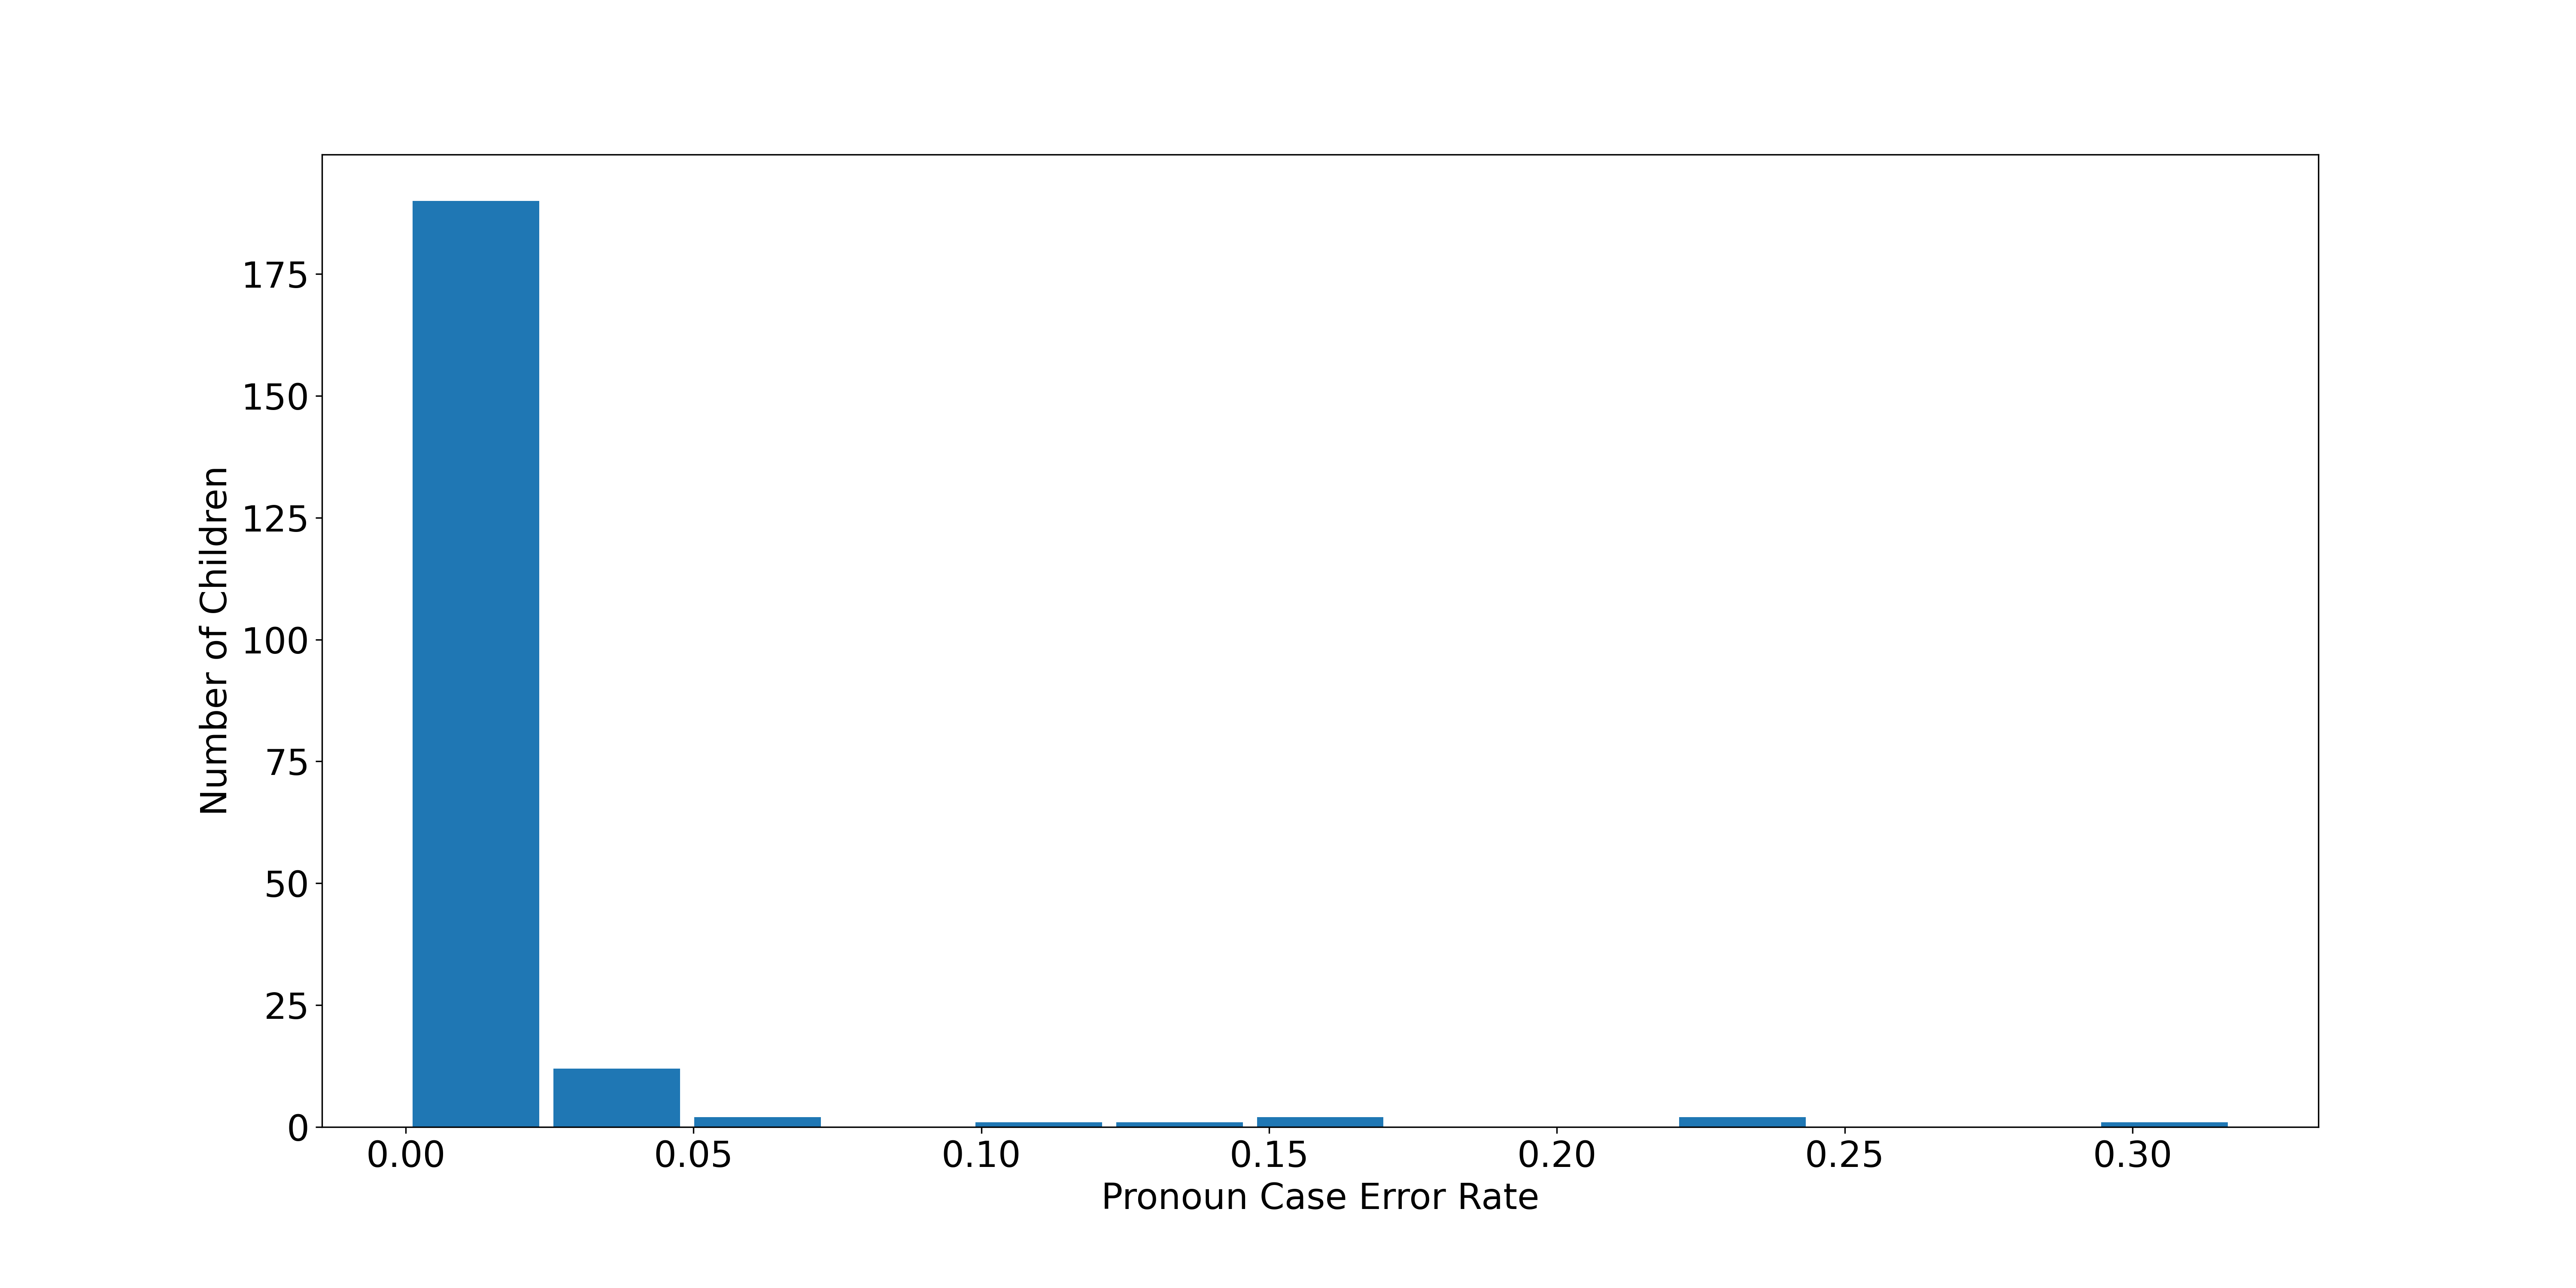
\includegraphics[scale = 0.35]{graph/OverallErrorRate.png}
\vspace{-3em}
\caption{Histogram of pronoun case error rate among 211 children}
\label{fig:212}
\end{figure}
\FloatBarrier
\begin{figure}[h]
\centering
    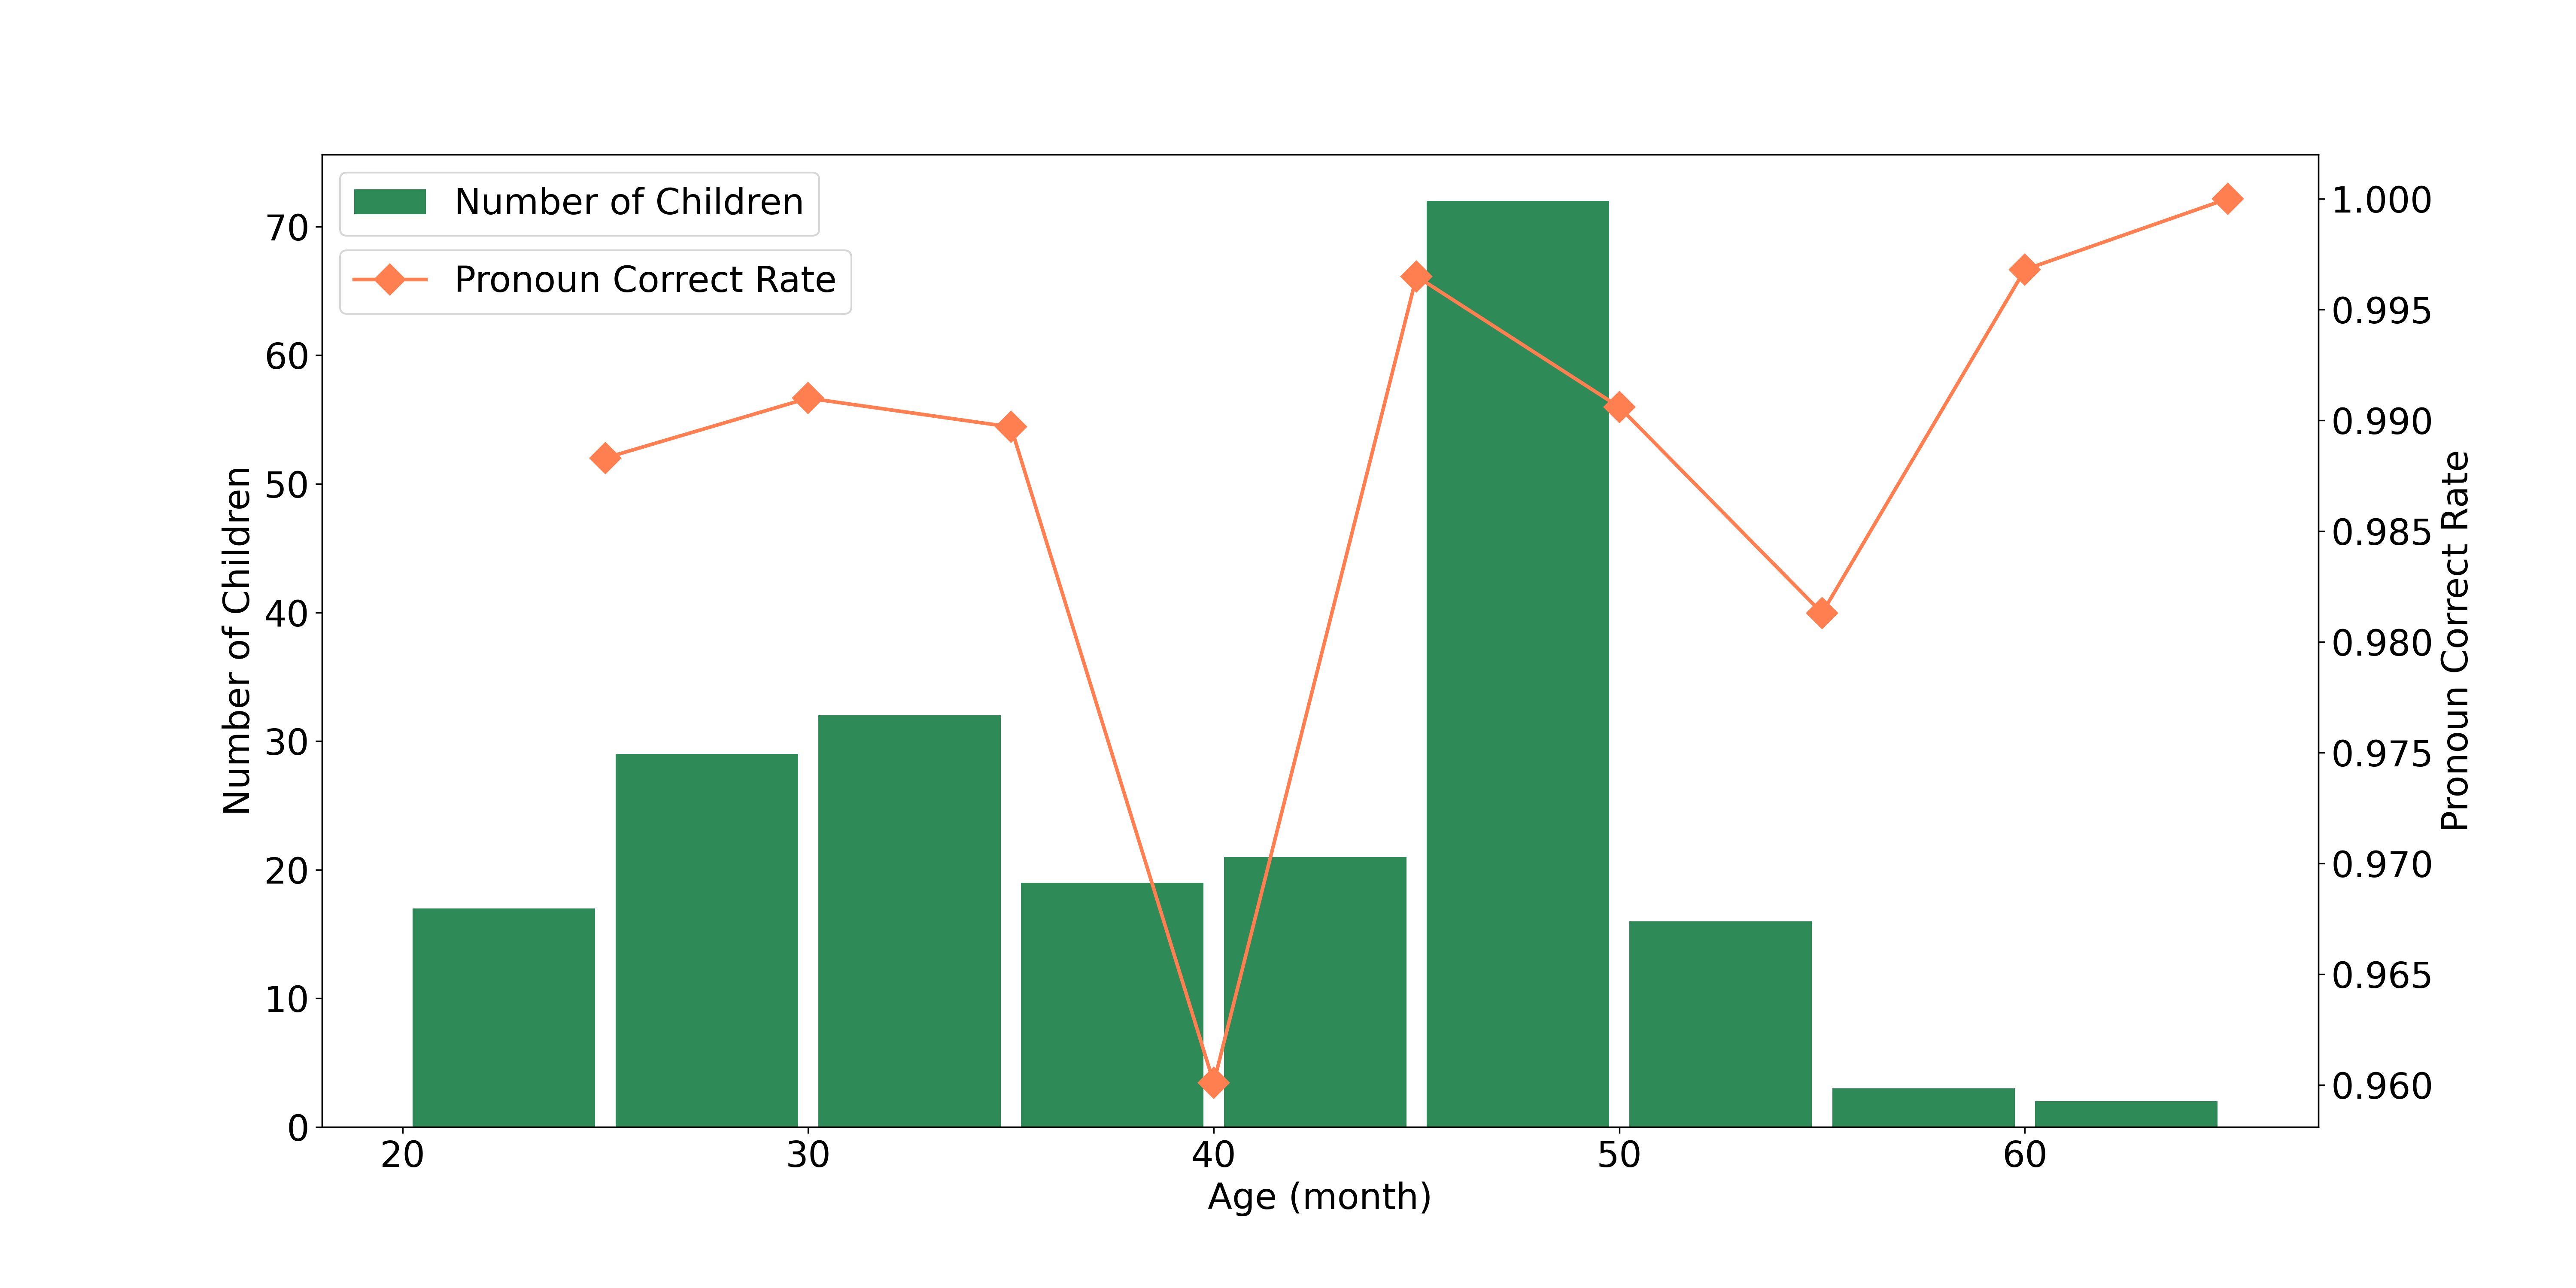
\includegraphics[scale =0.35] {graph/Crosssectional.png}
    \vspace{-3em}
    \caption{Histogram of Age with Pronoun Correct Rate}
    \label{fig:cross}
\end{figure}
\subsubsection{The Rate of Pronoun Case Errors from Longtitudinal Data}
Table \ref{table:2} shows a summary of each longitudinal child's age and MLU range, total number of pronoun and pronoun errors and total number of pronoun produced by their parents. The average pronoun case correct rate is 98.44\% and the median correct rate is 99.40\%, suggesting that most of the children rarely make any pronoun case errors. 

In order to examine if there's a U-shaped pattern for pronoun correct rate, files with the same age month were concatenated as one age point. For example, Eleanor in the dense MPI corpus \citep{rowland2006effect} had 19 files at the age of 2;0. The MLU, children's total pronouns, total input pronouns, total errors and pronoun correct rate are averaged over the 19 files to represent the age point 2;0. First, Spearman's rho test was conducted to calculate the correlation between the pronoun correct rate with age, MLU, children's total pronouns and total input pronouns at each age point. As shown in Table \ref{table:3}, the pronoun correct rate for 46 children has a complicated relationship with age, mlu, children's total words, children's total pronouns and parents' input pronouns. For 27 children, a significant correlation was found between pronoun correct rate VS age, mlu, children's total words, children's total pronouns and input pronouns. 9 children's age and mlu are both positively correlated with pronoun correct rate. 3 children's age and mlu are both negatively correlated with pronoun correct rate. 
3 children's (Fraser, Stuart, She) pronoun correct rate was only positively correlated with age, but not MLU. Nathaniel's pronoun correct rate is only positively correlated with MLU but not age. Conor's MLU is negatively correlated with pronoun correct rate. In addition, the age range doesn't seem to affect the correlation. For example, Aran, Dominic and John from the Manchester corpus \citep{theakston2001} all have the same age range (1;11 - 2;11) and 12 age points; Aran's pronoun correct rate is positively correlated with age and mlu; Dominic's pronoun correct rate is negatively correlated with age and mlu; while there is no significant correlation between John's pronoun correct rate and age or mlu. 

Similarly, both negative and positive correlations were found between pronoun correct rate VS children's total words, children's total pronouns and children's input pronouns; and for more than half of the children, there is no significant correlation between pronoun correct rate VS children's total words, children's total pronouns and children's input pronouns. 

Given that there is no unified monotonic improvement in pronoun correct rate with age and mlu, it is possible that the pronoun correct rate would show a U-shaped pattern on longitudinal data. 9 children with at least 20 age points (Thomas, Laura, Adam, Sarah, Naomi, Ross, Abe, Matt, Roman) were selected for plotting pronoun correct rate and age. The 9 children's age range varies. For example, Ross's age point starts at 1;4 and ends at 7;8, while Abe's age point starts at 2;5 and ends 5;0. To ensure that all 9 children are fairly represented on the graph, the most common age range 2;4 - 5;0 (with 32 age points) was selected. Each child's pronoun correct rate at different age points are plotted in Figure \ref{fig:1}. The detailed data can be found in Table \ref{table:4}. 
\vspace{-1em}
\FloatBarrier
\begin{figure}[!h]
\small
\centering
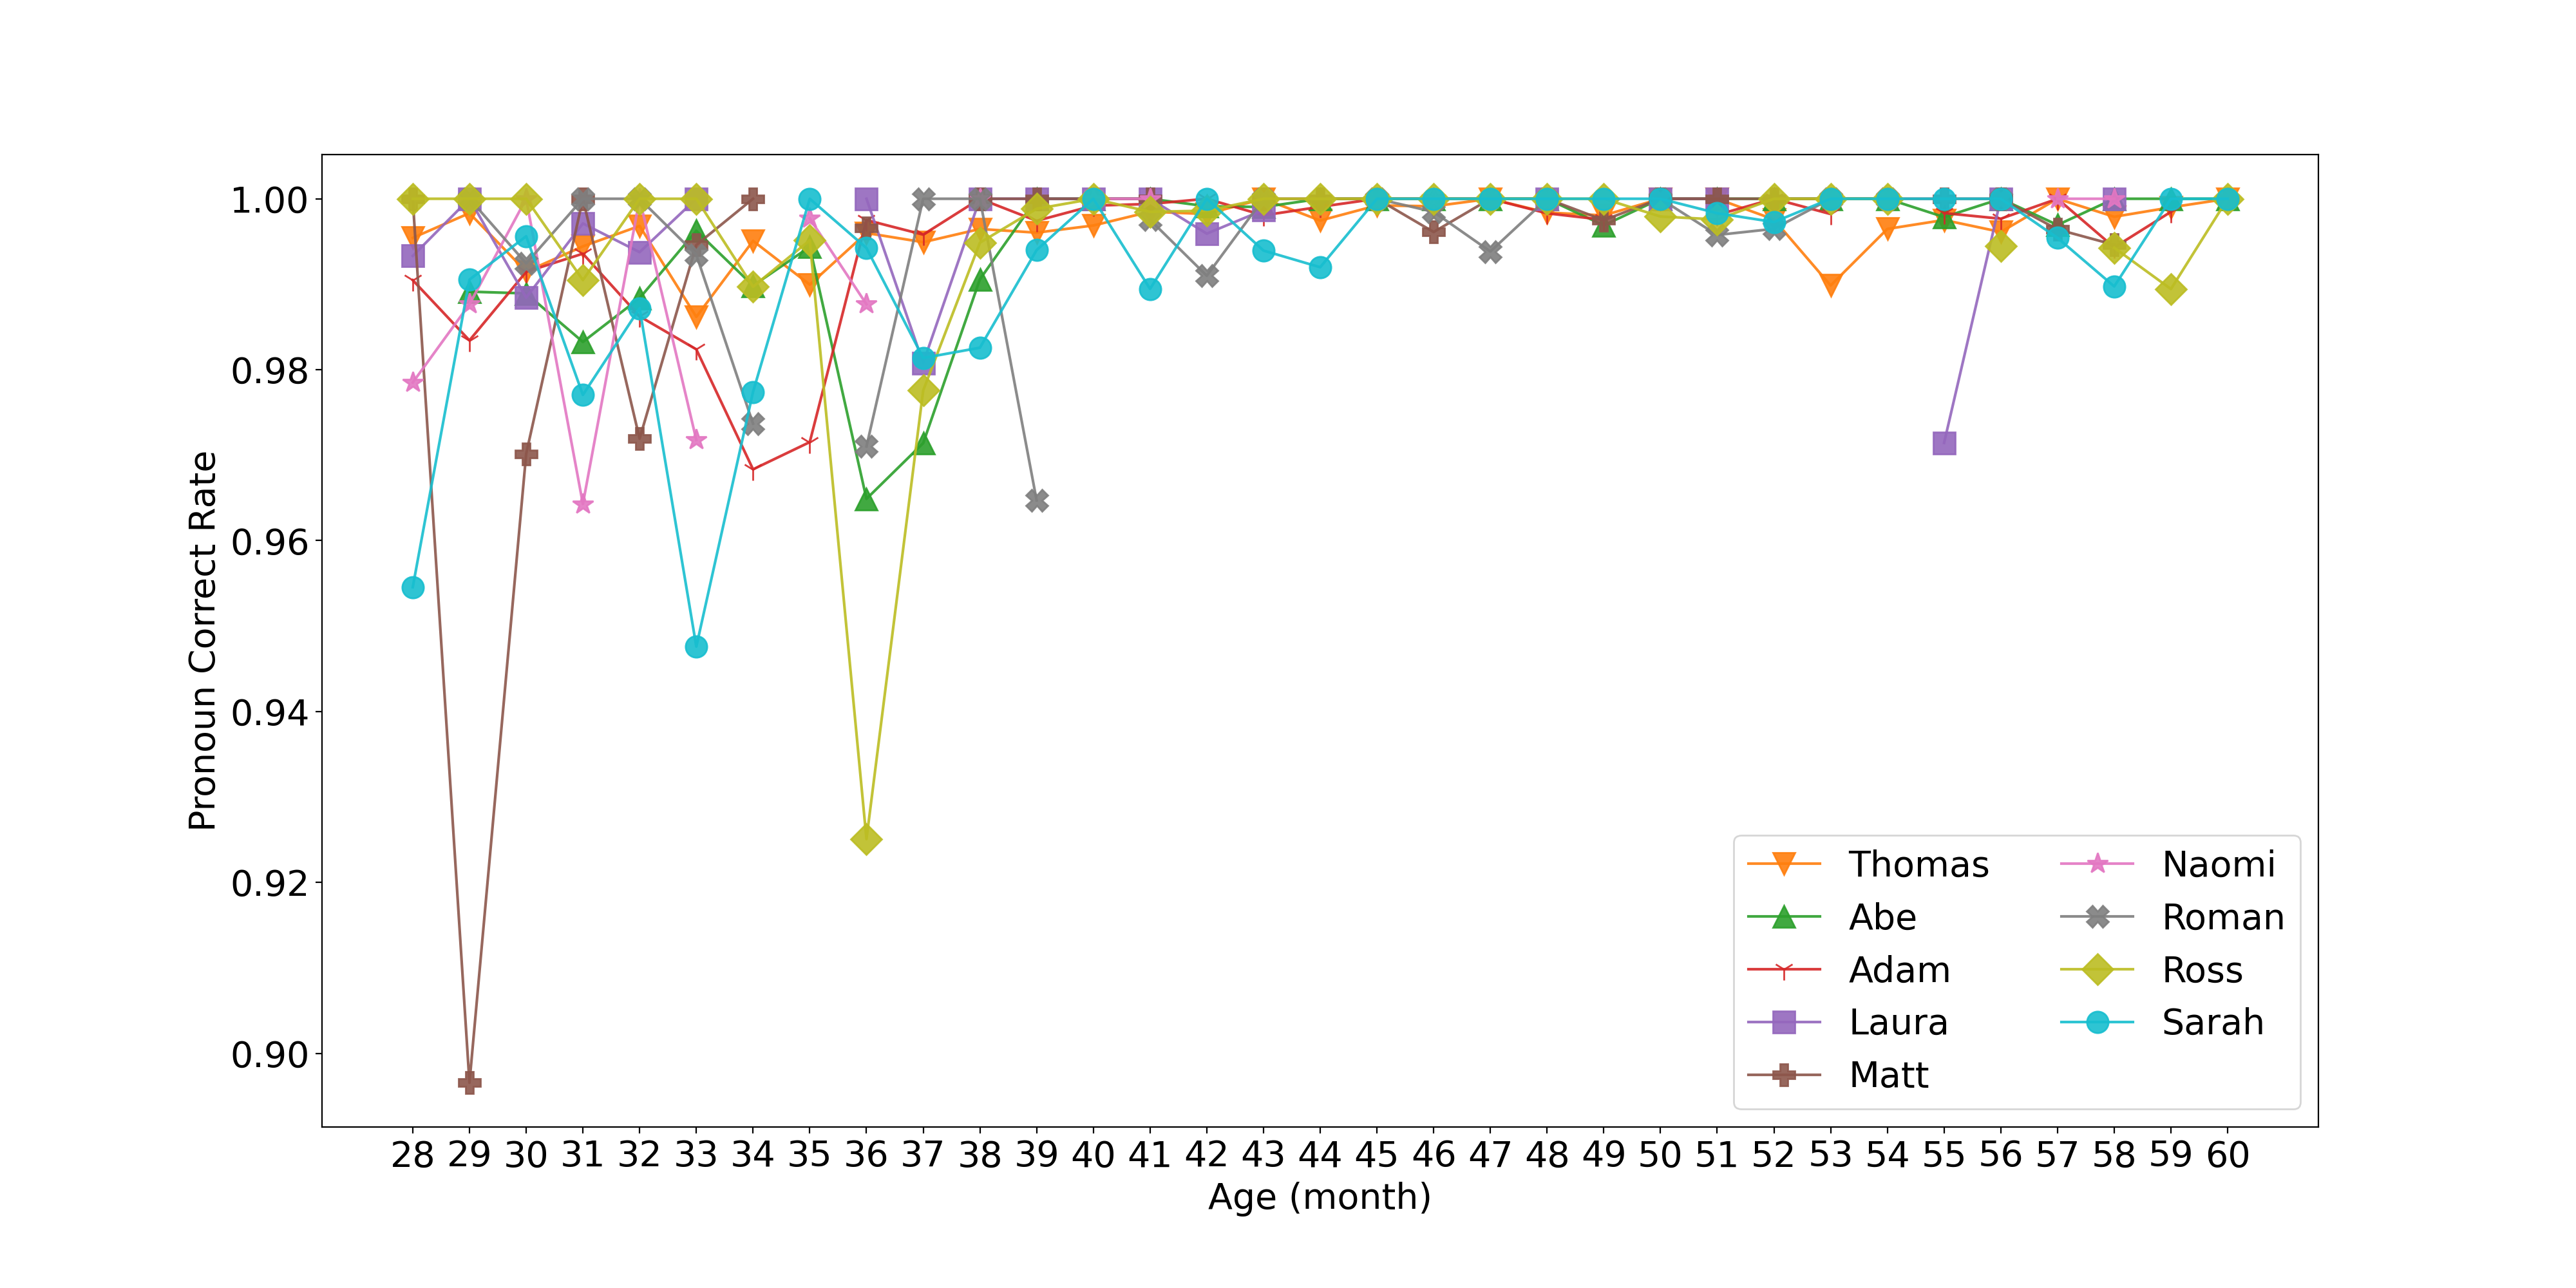
\includegraphics[scale = 0.35, width = \linewidth]{graph/Age1month.png}
\vspace{-2em}
\caption{Age and Pronoun Correct Rate per age point for longitudinal data and cross-sectional data }
\label{fig:1}
\end{figure}
\FloatBarrier

The pronoun correct rate has a very noisy pattern at the early age points and stabilizes roughly after the age point of 3;4 (40 months). To get a clearer visualization for the early age points, the pronoun correct rates were averaged per 5 age points and the new plot is shown in Figure \ref{fig:2}.
\FloatBarrier
\begin{figure}[h]
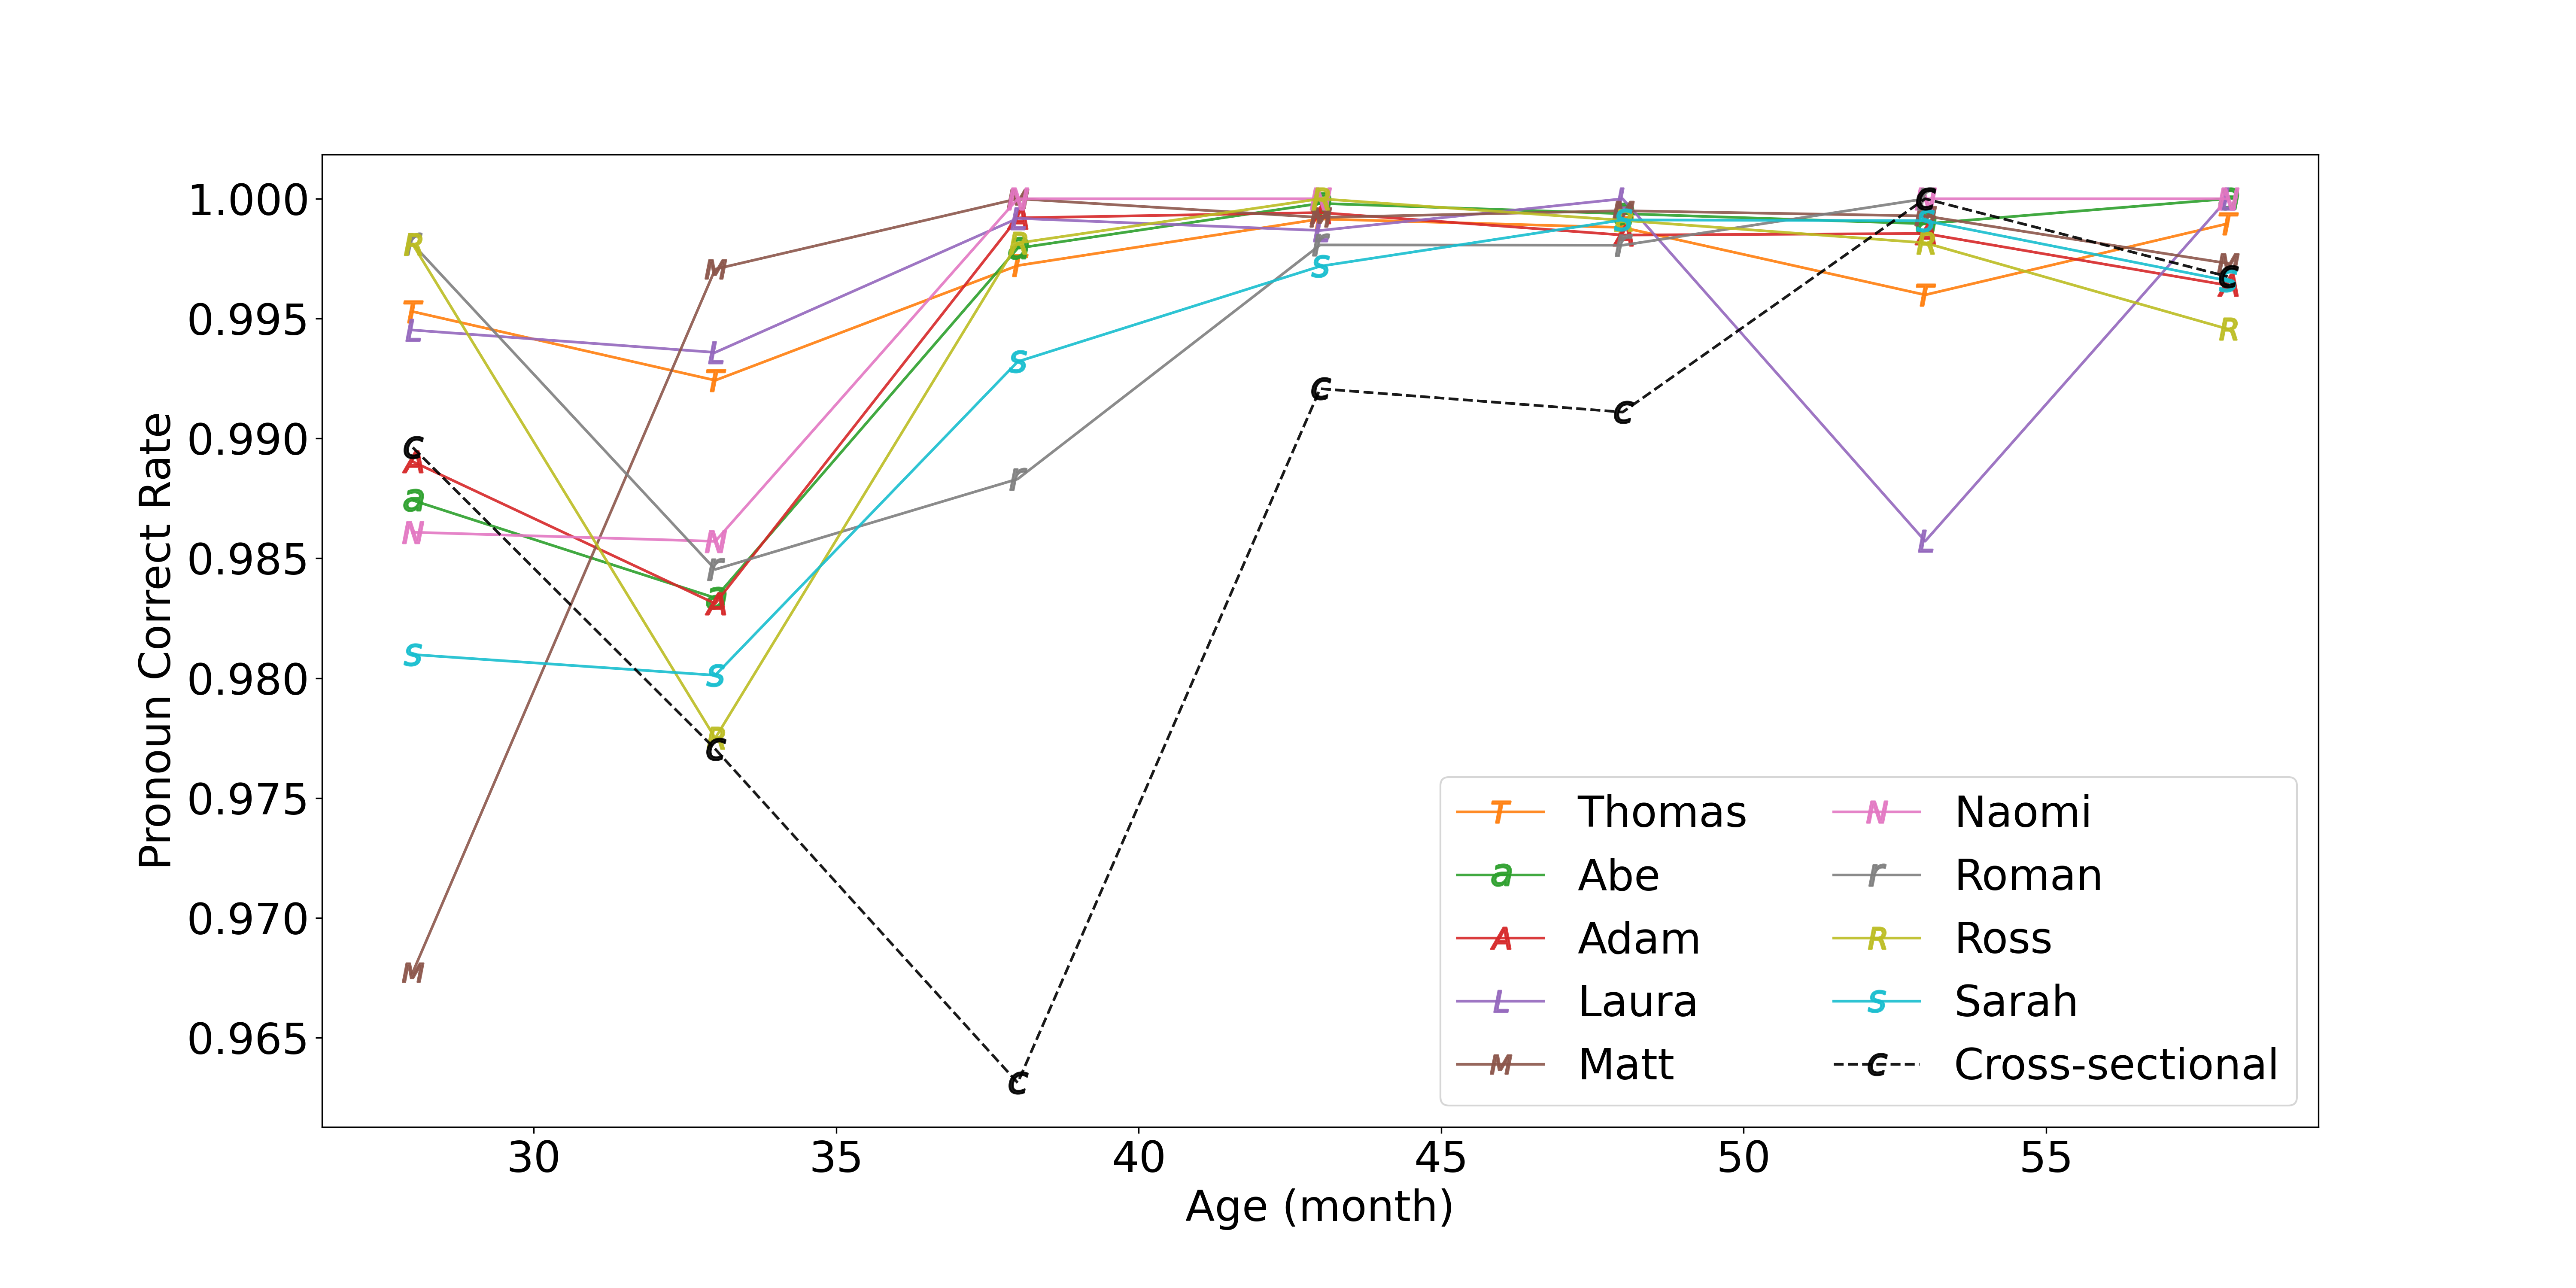
\includegraphics[scale = 0.35, width = \linewidth]{graph/Age5month.png}
\vspace{-2em}
\caption{Age and Pronoun Correct Rate per 5 age points}
\label{fig:2}
\end{figure}
\FloatBarrier
The colored solid lines represent each individual child's pronoun correct rate and the dashed black line represents the cross-sectional data. The longitudinal children's pronoun correct rate seems to resemble a U-shaped pattern, that most children start with a relatively high correct rate and then experience a dip at around age 2;9 (33 months) and return to high correct rate roughly after 3;7 (40 months). However, the position of the dip in longitudinal data is slightly different from the dip in the cross-sectional data: the pronoun correct rate dropped earlier for the children with longitudinal data than the children with cross-sectional data. It is unclear why the pronoun correct rate dropped at different ages for longitudinal children and cross-sectional children. 

\FloatBarrier
\begin{table}[h]
\centering
\small
\caption{Summary of children's age range, mlu range, total pronouns, total input pronouns and total errors}
\label{table:2}
\begin{tabular}{llllllll}
\hline
\textbf{Name} & \textbf{{\begin{tabular}[c]{@{}l@{}}Total\\files \end{tabular}}}\footnote{Diary files were not included in this study. For example, Lara had 225 diary files that were not included in the study.} & \textbf{Age range} & \textbf{MLU range} & \textbf{\begin{tabular}[c]{@{}l@{}}Children's\\ Total\\ Pronoun\end{tabular}} & \textbf{\begin{tabular}[c]{@{}l@{}}Total\\Input\\ pronoun\end{tabular}} & \textbf{{\begin{tabular}[c]{@{}l@{}}Total\\Errors \end{tabular}}} & \textbf{\begin{tabular}[c]{@{}l@{}}Correct \\ Rate\end{tabular}} \\ \hline
Anne & 40 & 1;10 - 2;9 & 1.75 - 4.15 & 4957 & 18707 & 54 & 98.91\% \\
Aran & 53 & 1;11 - 2;11 & 1.46 - 5.02 & 10174 & 43339 & 24 & 99.76\% \\
Barbara & 14 & 2;4 - 4;2 & 3.37 - 6.47 & 1339 & 5052 & 7 & 99.48\% \\
Becky & 35 & 2;0 - 2;11 & 1.53 - 3.97 & 6893 & 14524 & 41 & 99.41\% \\
Carl & 33 & 1;9 - 2;8 & 2.22 - 4.36 & 5446 & 10398 & 32 & 99.41\% \\
Conor & 14 & 3;8 - 4;6 & 1.87 - 5.71 & 1993 & 8051 & 14 & 99.30\% \\
Courtney & 7 & 3;4 - 4;0 & 5.13 - 6.68 & 1398 & 1727 & 6 & 99.57\% \\
David & 14 & 2;0 - 4;2 & 2.32 - 6.41 & 1013 & 3219 & 3 & 99.70\% \\
Dominic & 36 & 1;11 - 2;11 & 1.34 - 4.08 & 4787 & 18519 & 47 & 99.02\% \\
Eleanor & 181 & 2;0 - 3;1 & 2.12 - 4.25 & 28834 & 59462 & 80 & 99.72\% \\
Fraser & 217 & 2;0 - 3;1 & 1.70 - 5.7 & 37480 & 92975 & 67 & 99.82\% \\
Gail & 35 & 2;0 - 2;11 & 1.87 - 4.33 & 4690 & 16029 & 63 & 98.66\% \\
Joel & 35 & 1;11 - 2;10 & 1.41 - 3.92 & 4936 & 15207 & 24 & 99.51\% \\
John & 32 & 1;11 - 2;11 & 1.92 - 3.78 & 2168 & 10276 & 8 & 99.63\% \\
Johnny & 7 & 3;6 - 4;4 & 3.93 - 4.52 & 861 & 507 & 4 & 99.54\% \\
Lara & 125 & 1;9 - 3;4 & 1.85 - 5.35 & 153054 & 40920 & 63 & 99.75\% \\
Liz & 34 & 1;11 - 2;11 & 1.52 - 4.79 & 5048 & 10708 & 31 & 99.39\% \\
Michelle & 14 & 2;5 - 4;5 & 3.0 - 6.87 & 2386 & 3979 & 31 & 98.70\% \\
Nicole & 34 & 2;1 - 3;0 & 1.26 - 3.61 & 2286 & 17860 & 51 & 97.77\% \\
Rachel & 9 & 2;6 - 3;2 & 2.8 - 6.33 & 663 & 2756 & 42 & 93.67\% \\
Ruth & 33 & 1;11 - 3;0 & 1.63 - 4.34 & 4077 & 19657 & 971 & 76.18\% \\
Stuart & 11 & 3;5 - 4;5 & 4.51 - 6.34 & 2352 & 2720 & 22 & 99.06\% \\
Thomas & 379 & 2;0 - 5;0 & 1.55 - 6.92 & 48115 & 226908 & 197 & 99.59\% \\
Warren & 36 & 1;10 - 2;10 & 2.02 - 4.71 & 4008 & 14818 & 96 & 97.60\% \\
Peter & 20 & 1;9 - 3;2 & 1.47 - 6.66 & 7637 & 2527 & 89 & 98.83\% \\
Laura & 200 & 1;5 - 7;0 & 1.0 - 6.69 & 9895 & 14280 & 82 & 99.17\% \\
Adam & 55 & 2;3 - 5;2 & 2.41 - 6.48 & 23726 & 13172 & 90 & 99.62\% \\
Eve & 20 & 1;6 - 2;3 & 2.1 - 4.99 & 4217 & 6458 & 39 & 99.08\% \\
Sarah & 139 & 2;3 - 5;1 & 1.59 - 7.77 & 15344 & 18512 & 110 & 99.28\% \\
Jimmy & 26 & 2;2 - 2;10 & 3.51 - 5.8 & 2702 & 3736 & 31 & 98.85\% \\
Shem & 47 & 2;3 - 3;2 & 4.32 - 12.03 & 9176 & 2207 & 19 & 99.79\% \\
Naomi & 93 & 1;3 - 4;9 & 1.3 - 7.79 & 5200 & 6466 & 60 & 98.85\% \\
Ross & 409 & 1;4 - 7;8 & 1.7 - 21.25 & 24560 & 41774 & 99 & 99.60\% \\
She & 10 & 1;8 - 2;5 & 2.23 - 3.54 & 706 & 2355 & 21 & 97.03\% \\
Tow & 10 & 1;7 - 2;5 & 1.86 - 5.08 & 946 & 3790 & 34 & 96.41\% \\
Nina & 52 & 2;0 - 3;4 & 2.26 - 6.17 & 11740 & 25694 & 501 & 95.73\% \\
Abe & 210 & 2;5 - 5;0 & 3.69 - 10.58 & 24547 & 18526 & 130 & 99.47\% \\
Trevor & 26 & 2;1 - 4;0 & 4.28 - 8.12 & 2819 & 5222 & 17 & 99.40\% \\
Ben & 11 & 2;4 - 3;4 & 4.97 - 6.88 & 1634 & 1177 & 50 & 96.94\% \\
Emily & 23 & 2;6 - 4;6 & 4.66 - 9.54 & 5067 & 144 & 15 & 99.70\% \\
Emma & 27 & 2;8 - 4;8 & 3.71 - 6.4 & 3458 & 2648 & 5 & 99.86\% \\
Jillian & 22 & 2;1 - 2;10 & 2.76 - 7.16 & 2669 & 2795 & 5 & 99.81\% \\
Matt & 57 & 2;3 - 5;0 & 2.89 - 11.29 & 6586 & 19759 & 34 & 99.48\% \\
Roman & 42 & 2;3 - 4;8 & 2.98 - 12.11 & 6047 & 4745 & 33 & 99.45\% \\
Nathaniel & 47 & 2;6 - 3;9 & 1.82 - 6.45 & 2193 & 10329 & 14 & 99.36\% \\
Geraldine & 10 & 1;6 - 2;5 & 1.35 - 5.43 & 598 & 1945 & 3 & 99.50\% \\ \hline
\end{tabular}
\end{table}
\FloatBarrier

\FloatBarrier
\begin{table}[]
\small
\centering
\caption{Spearman's Correlation between Pronoun Correct Rate and Age, MLU, Children's total word production, Children's pronoun production, Total Input Pronouns}
\label{table:3}
\begin{tabular}{ll|lllll}
\toprule
 & &\multicolumn{5}{c}{\textbf{Correlation (r) with Pronoun Correct Rate}} \\
\hline
\textbf{Child} & \textbf{{\begin{tabular}[c]{@{}l@{}}N (age points)\\(age range)\end{tabular}}}& \textbf{Age} & \textbf{MLU} & \textbf{\begin{tabular}[c]{@{}l@{}}Children's\\ Total Words\end{tabular}} & \textbf{\begin{tabular}[c]{@{}l@{}}Children's\\ Total Pronouns\end{tabular}} & \textbf{\begin{tabular}[c]{@{}l@{}}Total Input\\ Pronouns\end{tabular}}\\
\hline
Anne&11 (1;10 - 2;9)&-0.16&-0.04&-0.38&-0.33&-0.29\\
Aran&12 (1;11 - 2;11)&\textbf{0.77**}&\textbf{0.68*}&\textbf{0.79**}&\textbf{0.78**}&-0.05\\
Barbara&10 (2;4 - 4;2)&-0.14&0.3&-0.12&-0.08&-0.08\\
Becky&12 (2;0 - 2;11)&-0.36&-0.57&-0.31&-0.34&0.49\\
Carl&12 (1;9 - 2;8)&-0.07&0.22&0.19&-0.02&0.42\\
Conor&9 (3;8 - 4;6)&-0.34&\textbf{-0.94***}&-0.38&-0.42&-0.43\\
Courtney&5 (3;4 - 4;0)&0&0&-0.35&-0.35&0\\
David&12 (2;0 - 4;2)&-0.16&-0.23&-0.44&-0.38&0.19\\
Dominic&12 (1;11 - 2;11)&\textbf{-0.77**}&\textbf{-0.77**}&\textbf{-0.62*}&\textbf{-0.81**}&-0.46\\
Eleanor&14 (2;0 - 3;1)&0.45&0.42&0.5&0.52&\textbf{0.83***}\\
Fraser&14 (2;0 - 3;1)&\textbf{0.60*}&0.5&0.42&\textbf{0.57*}&\textbf{0.57*}\\
Gail&11 (2;0 - 2;11)&0.35&0.25&\textbf{-0.43*}&-0.11&\textbf{0.51*}\\
Joel&11 (1;11 - 2;10)&0.12&0.09&0.31&0.11&\textbf{0.75**}\\
John&12 (1;11 - 2;11)&0&-0.02&-0.35&-0.11&0.08\\
Johnny&5 (3;6 - 4;4)&-0.15&-0.67&-0.36&-0.67&-0.67\\
Lara&19 (1;9 - 3;4)&\textbf{0.61**}&\textbf{0.60**}&0.3&\textbf{0.55*}&0.33\\
Liz&12 (1;11 - 2;11)&0.46&0.39&-0.12&0.15&-0.35\\
Michelle&9 (2;5 - 4;5)&-0.39&-0.14&-0.31&-0.31&0.29\\
Nicole&11 (2;1 - 3;0)&\textbf{-0.85***}&\textbf{-0.85***}&\textbf{-0.76***}&\textbf{-0.82***}&-0.11\\
Rachel&5 (2;6 - 3;2)&0.72&0.87&-0.87&-0.36&0.1\\
Ruth&13 (1;11 - 3;0)&0.4&0.45&0.36&0.33&0.51\\
Stuart&7 (3;5 - 4;5)&\textbf{0.83*}&0.09&-0.25&-0.11&-0.04\\
Thomas&36 (2;0 - 5;0)&\textbf{0.51**}&\textbf{0.58**}&\textbf{0.39*}&\textbf{0.39*}&0.1\\
Warren&12 (1;10 - 2;10)&0.05&-0.03&0.09&0.24&0.29\\
Peter&14 (1;9 - 3;2)&0.11&0.15&0.07&0.09&-0.37\\
Laura&34 (1;5 - 7;0)&\textbf{0.60***}&\textbf{0.48**}&\textbf{0.57***}&\textbf{0.50**}&\textbf{0.40*}\\
Adam&31 (2;3 - 5;2)&\textbf{0.61***}&\textbf{0.62***}&\textbf{0.50**}&\textbf{0.45*}&0.11\\
Eve&10 (1;6 - 2;3)&\textbf{-0.74*}&\textbf{-0.69*}&\textbf{-0.66*}&\textbf{-0.67*}&-0.02\\
Sarah&35 (2;3 - 5;1)&\textbf{0.63***}&\textbf{0.60***}&\textbf{0.46**}&0.28&0.04\\
Jimmy&6 (2;2 - 2;10)&-0.6&-0.6&0.31&-0.09&0.31\\
Shem&12 (2;3 - 3;2)&0.04&-0.03&0.04&0.25&0.39\\
Naomi&23 (1;3 - 4;9)&\textbf{0.42*}&\textbf{0.43*}&0.25&0.33&0.18\\
Ross&62 (1;4 - 7;8)&0.14&-0.07&-0.17&-0.19&0.09\\
She&9 (1;8 - 2;5)&\textbf{0.78*}&0.57&0.45&\textbf{0.72*}&0.52\\
Tow&9 (1;7 - 2;5)&0.31&0.29&0&0&-0.15\\
Nina&15 (2;0 - 3;4)&\textbf{0.83***}&\textbf{0.86***}&\textbf{0.62*}&\textbf{0.68**}&0.26\\
Abe&32 (2;5 - 5;0)&\textbf{0.69***}&\textbf{0.38*}&-0.26&-0.24&\textbf{-0.46**}\\
Trevor&10 (2;1 - 4;0)&0.01&-0.49&-0.07&-0.05&0.25\\
Ben&8 (2;4 - 3;4)&0.36&0.4&-0.19&0.5&\textbf{0.71*}\\
Emily&13 (2;6 - 4;6)&0.07&-0.18&-0.4&-0.37&-0.25\\
Emma&16 (2;8 - 4;8)&0.47&0.41&0.44&0.43&-0.21\\
Jillian&7 (2;1 - 2;10)&-0.08&-0.16&-0.45&-0.35&0.37\\
Matt&29 (2;3 - 5;0)&0.27&0.28&0.29&0.11&0.09\\
Roman&24 (2;3 - 4;8)&0.15&-0.06&-0.19&-0.07&0.17\\
Nathaniel&10 (2;6 - 3;9)&0.35&\textbf{0.63*}&0.12&0.52&0.22\\
Geraldine&7 (1;6 - 2;5)&0.4&0.4&-0.04&0.09&0.04\\
\bottomrule
\end{tabular}
\end{table}
\FloatBarrier


\FloatBarrier
\begin{table}[h]
\small
\centering
\caption{Pronoun Correct Rate at each age points for 9 children}
\label{table:4}
\begin{tabular}{c|lllllllll}
\hline
\textbf{{\begin{tabular}[c]{@{}c@{}}Age\\(month)\end{tabular}}} & \textbf{Thomas} & \textbf{Abe} & \textbf{Adam} & \textbf{Laura} & \textbf{Matt} & \textbf{Naomi} & \textbf{Roman} & \textbf{Ross} & \textbf{Sarah} \\ 
\toprule
28 & 0.9954 & N/A & 0.9905 & 0.9933 & 1 & 0.9785 & N/A & 1 & 0.9545 \\
29 & 0.9983 & 0.9891 & 0.9834 & 1 & 0.8966 & 0.9877 & 1 & 1 & 0.9905 \\
30 & 0.9915 & 0.9889 & 0.9915 & 0.9884 & 0.9701 & 1 & 0.9924 & 1 & 0.9956 \\
31 & 0.9944 & 0.9832 & 0.9936 & 0.9971 & 1 & 0.9643 & 1 & 0.9905 & 0.9770 \\
32 & 0.9968 & 0.9884 & 0.9862 & 0.9938 & 0.9719 & 1 & 1 & 1 & 0.9872 \\
33 & 0.9862 & 0.9962 & 0.9824 & 1 & 0.9946 & 0.9718 & 0.9934 & 1 & 0.9476 \\
34 & 0.9951 & 0.9898 & 0.9683 & N/A & 1 & N/A & 0.9737 & 0.9897 & 0.9774 \\
35 & 0.9900 & 0.9944 & 0.9715 & N/A & N/A & 0.9977 & N/A & 0.9951 & 1 \\
36 & 0.9960 & 0.9649 & 0.9975 & 1 & 0.9966 & 0.9877 & 0.9710 & 0.9251 & 0.9942 \\
37 & 0.9949 & 0.9714 & 0.9958 & 0.9808 & N/A & N/A & 1 & 0.9776 & 0.9814 \\
38 & 0.9965 & 0.9906 & 1 & 1 & 1 & 1 & 1 & 0.9949 & 0.9826 \\
39 & 0.9960 & 1 & 0.9974 & 1 & 1 & N/A & 0.9647 & 0.9988 & 0.9940 \\
40 & 0.9969 & 1 & 0.9992 & 1 & 1 & 1 & N/A & 1 & 1 \\
41 & 0.9985 & 1 & 0.9994 & 1 & 1 & 1 & 0.9975 & 0.9985 & 0.9895 \\
42 & 0.9982 & 0.9991 & 1 & 0.9959 & N/A & N/A & 0.9910 & 0.9986 & 1 \\
43 & 1 & 0.9990 & 0.9981 & 0.9987 & 1 & N/A & 1 & 1 & 0.9939 \\
44 & 0.9974 & 1 & 0.9991 & N/A & 1 & N/A & N/A & 1 & 0.9920 \\
45 & 0.9992 & 1 & 1 & N/A & 1 & N/A & 1 & 1 & 1 \\
46 & 0.9991 & 1 & 1 & N/A & 0.9961 & 1 & 0.9985 & 1 & 1 \\
47 & 1 & 1 & 1 & N/A & 1 & N/A & 0.9938 & 1 & 1 \\
48 & 0.9984 & 1 & 0.9983 & 1 & 1 & N/A & 1 & 1 & 1 \\
49 & 0.9981 & 0.9969 & 0.9975 & N/A & 0.9975 & N/A & N/A & 1 & 1 \\
50 & 1 & 1 & N/A & 1 & 1 & N/A & 1 & 0.9979 & 1 \\
51 & 1 & 1 & 0.9981 & 1 & 1 & N/A & 0.9958 & 0.9976 & 0.9983 \\
52 & 0.9976 & 1 & 1 & N/A & 1 & N/A & 0.9965 & 1 & 0.9973 \\
53 & 0.9899 & 1 & 0.9982 & N/A & 1 & N/A & 1 & 1 & 1 \\
54 & 0.9965 & 1 & N/A & N/A & 1 & N/A & 1 & 1 & 1 \\
55 & 0.9975 & 0.9979 & 0.9983 & 0.9714 & 1 & N/A & N/A & N/A & 1 \\
56 & 0.9961 & 1 & 0.9977 & 1 & 1 & N/A & 1 & 0.9945 & 1 \\
57 & 1 & 0.9969 & 1 & N/A & 0.9964 & 1 & N/A & N/A & 0.9954 \\
58 & 0.9979 & 1 & 0.9943 & 1 & 0.9946 & 1 & N/A & 0.9943 & 0.9897 \\
59 & 0.9990 & 1 & 0.9985 & N/A & N/A & N/A & N/A & 0.9894 & 1 \\
60 & 1 & 1 & N/A & N/A & 1 & N/A & N/A & 1 & 1 \\ 
\bottomrule
\end{tabular}
\end{table}
\FloatBarrier

\subsubsection{Do Pronoun Case Errors Display a U-shaped Pattern?}
The U-shaped developmental trajectory has been observed in a wide variety of learning contexts \citep[for a review, see][]{siegler2004u}. It is especially interesting in language development since it contradicts the idea that language acquisition is monotonic. If the pronoun case errors display a U-shaped pattern, explanations for such errors should account for the non-monotonic developmental pattern too, which provides an important criterion to evaluate the effectiveness of different explanations. 

It's difficult to judge whether the pronoun case errors follow a U-shaped pattern. One challenge is that there is no accurate definition of the U-shaped developmental curve. It has been loosely described as a three-step process: good performance followed by bad performance followed by good performance again. However, it's difficult to decide what is good performance and what is bad performance in the pronoun case error context where most of the children have an extremely low error rate. In Figure \ref{fig:2}, the plot does display the shape of `U', but the difference between the nadir (96.5\%) and the zenith (100\%) is so small that it is unclear whether there is meaningful improvement.

Most studies reporting a U-shaped developmental pattern did not plot the detailed correct rate with age to demonstrate that there is a U-shaped pattern. Instead, they showed that the performance at a later age is significantly worse than an earlier age, but eventually gets better. For example, \cite{namy2004changing} reported that both an 18-month group and a 4-year-old group had better performance on mapping arbitrary gestures than a 26-month-old group. In order to test if the pronoun correct rate at a certain age is  worse the other ages, all the months in cross-sectional data were divided into 7 groups with 5 months apart to ensure that each group have enough samples. Table \ref{table:KW} shows the mean and median pronoun correct rate for 7 different age groups. Since the error rates are not normally distributed and the sample size N for each group is different, a Kruskal-Wallis test (or one-way ANOVA on ranks) was used to compare the correct rate in different groups. The test result shows that there is no significant difference in pronoun correct rate among age groups, H(6) = 8.57, p = 0.20. This result suggests that even there is a dip of pronoun correct rate at around 2;9 - 3;2, the change is not significant. 
\FloatBarrier
\begin{table}[h]
\centering
\caption{Mean and Median Pronoun Correct Rate for 7 age groups }
\label{table:KW}
\begin{tabular}{llll}
\toprule
\begin{tabular}[c]{@{}c@{}}Age Group \\(month)\end{tabular} & N & Mean & Median \\
\hline
\textless{}26 & 18 & 98.83\% & 100\% \\
26 - 30 & 35 & 99.06\% & 100\%\\
31 - 35 & 29 & 98.97\% & 100\%\\
36 - 40 & 18 & 96.01\% & 100\% \\
41 - 45 & 32 & 99.65\% & 100\% \\
46 - 50 & 65 & 99.06\% & 100\% \\
\textgreater{}50 & 14 & 98.71\% & 100\%\\
\bottomrule
\end{tabular}
\end{table}
\FloatBarrier

In addition, a polynominal function was fitted onto the cross-sectional data. A significant quadratic component can be counted as an evidence for a U-shaped pattern. The fitted plot in Figure \ref{poly1} shows that the quadratic regression doesn't fit the cross-sectional data, $R^2$ = 0.006, F(2,208) = 0.58, p = 0.56.
\vspace{-1em}
\FloatBarrier
\begin{figure}[h]
    \centering
    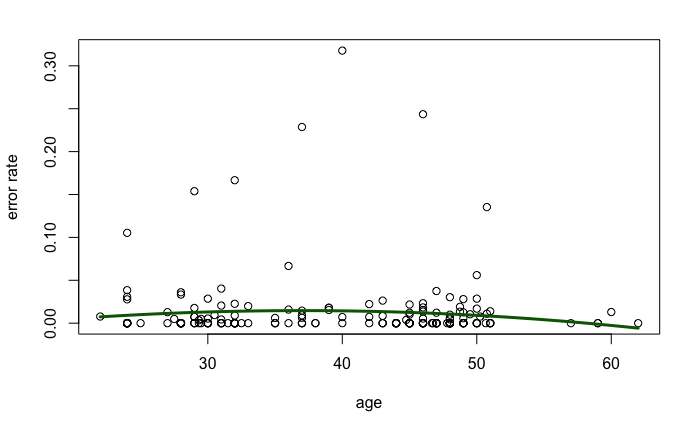
\includegraphics[scale = 0.5]{graph/polynominal1.png}
    \vspace{-1em}
    \caption{Quadratic Function for All Cross-sectional Data Points}
    \label{poly1}
\end{figure}
\FloatBarrier
One reason that the fitting is bad could be that the outliers, data points were the error rate is larger than 0.1, affect the fitting. Therefore, the quadratic function was fitted onto the cross-sectional data without data points with error rates larger than 0.1. The fitted plot is shown in Figure (\ref{poly2}), with $R^2$ = 0.001, F(2,201) = 0.09, p = 0.92. Excluding the outliers didn't improve the model.
\FloatBarrier
\begin{figure}[h]
    \centering
    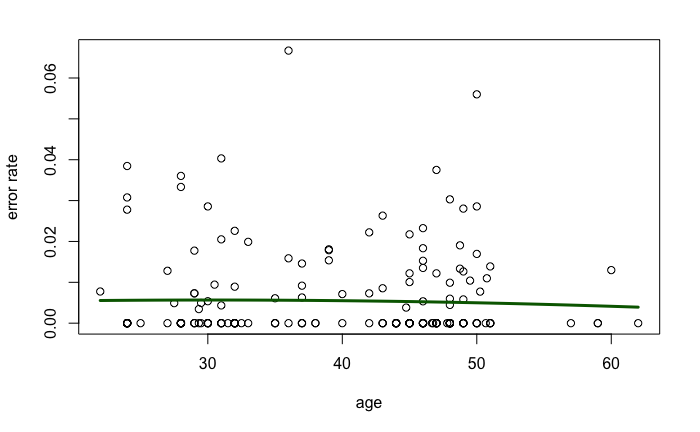
\includegraphics[scale = 0.5]{graph/polynominal2.png}
        \vspace{-1em}
    \caption{Quadratic Function for Cross-sectional Data without Error Rates < 0.1}
    \label{poly2}
\end{figure}
\FloatBarrier
Another reason for the poor fitting of quadratic regression could be that many children have 0 error rate. Therefore, the quadratic function was fitted onto the cross-sectional data without 0 error rate points. The fitted plot in Figure (\ref{poly3}) shows that excluding 0 error rate data points still couldn't make quadratic regression a good fitting model, $R^2$ = 0.01, F(2, 68) = 0.37, p = 0.69.
\FloatBarrier
\begin{figure}[h]
    \centering
    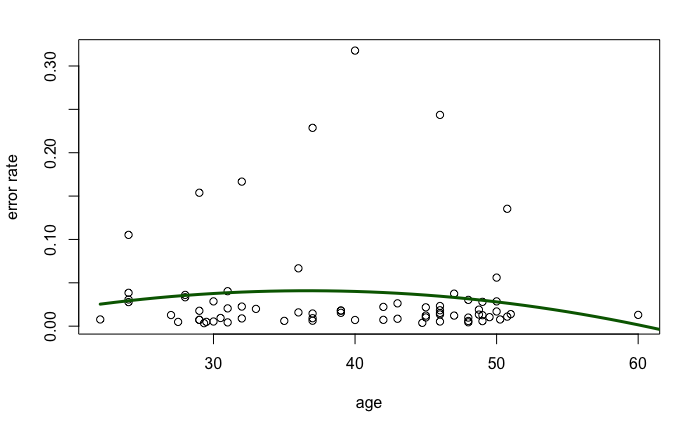
\includegraphics[scale = 0.5]{graph/polynomial3.png}
    \vspace{-1em}
    \caption{Quadratic Function for Cross-sectional Data without 0 Error Rates}
    \label{poly3}
\end{figure}
\FloatBarrier
The results of the Kruskal-Wallis test and the quadratic function fitting suggests that even though there is a dip in the pronoun case correct rate at around 2;9-3;2, the change is not significant. Based on the cross-sectional data, it's difficult to conclude that there is a U-shaped pattern. 


For longitudinal data, since there are not enough samples for different age groups,  Kruskal-Wallis test can not be used to test if the pronoun correct rate is significantly different at different ages. Instead, the longitudinal change in the pronoun correct rate was compared to the correct rate on past-tense verbs. \cite{marcus1992overregularization}'s study on past-tense verb overregularization errors reported a U-shaped development pattern with detailed correct rate over 4 children's (Adam, Eve, Sarah, Abe) longitudinal data. To compare the shape and change of correct rate, Adam's, Sarah's and Abe's past-tense verb correct rate and pronoun correct rate were plotted together in Figure \ref{fig:3}. The pronoun correct rate stabilized above 95\% for all ages, while verb correct rate is more has more variations at different age points. Again, the comparison with past-tense verb correct rate shows that the changes in pronoun correct rate are too small.  

In sum, the plot between age and pronoun correct rate displays the shape of `U' in both longitudinal and cross-sectional data. However, the pronoun correct rate at different ages are all very close to 100\%, making the change in the correct rate not so meaningful. Therefore, no conclusion about U-shaped developmental pattern can be drawn. 
 

\FloatBarrier
\begin{figure}[h]
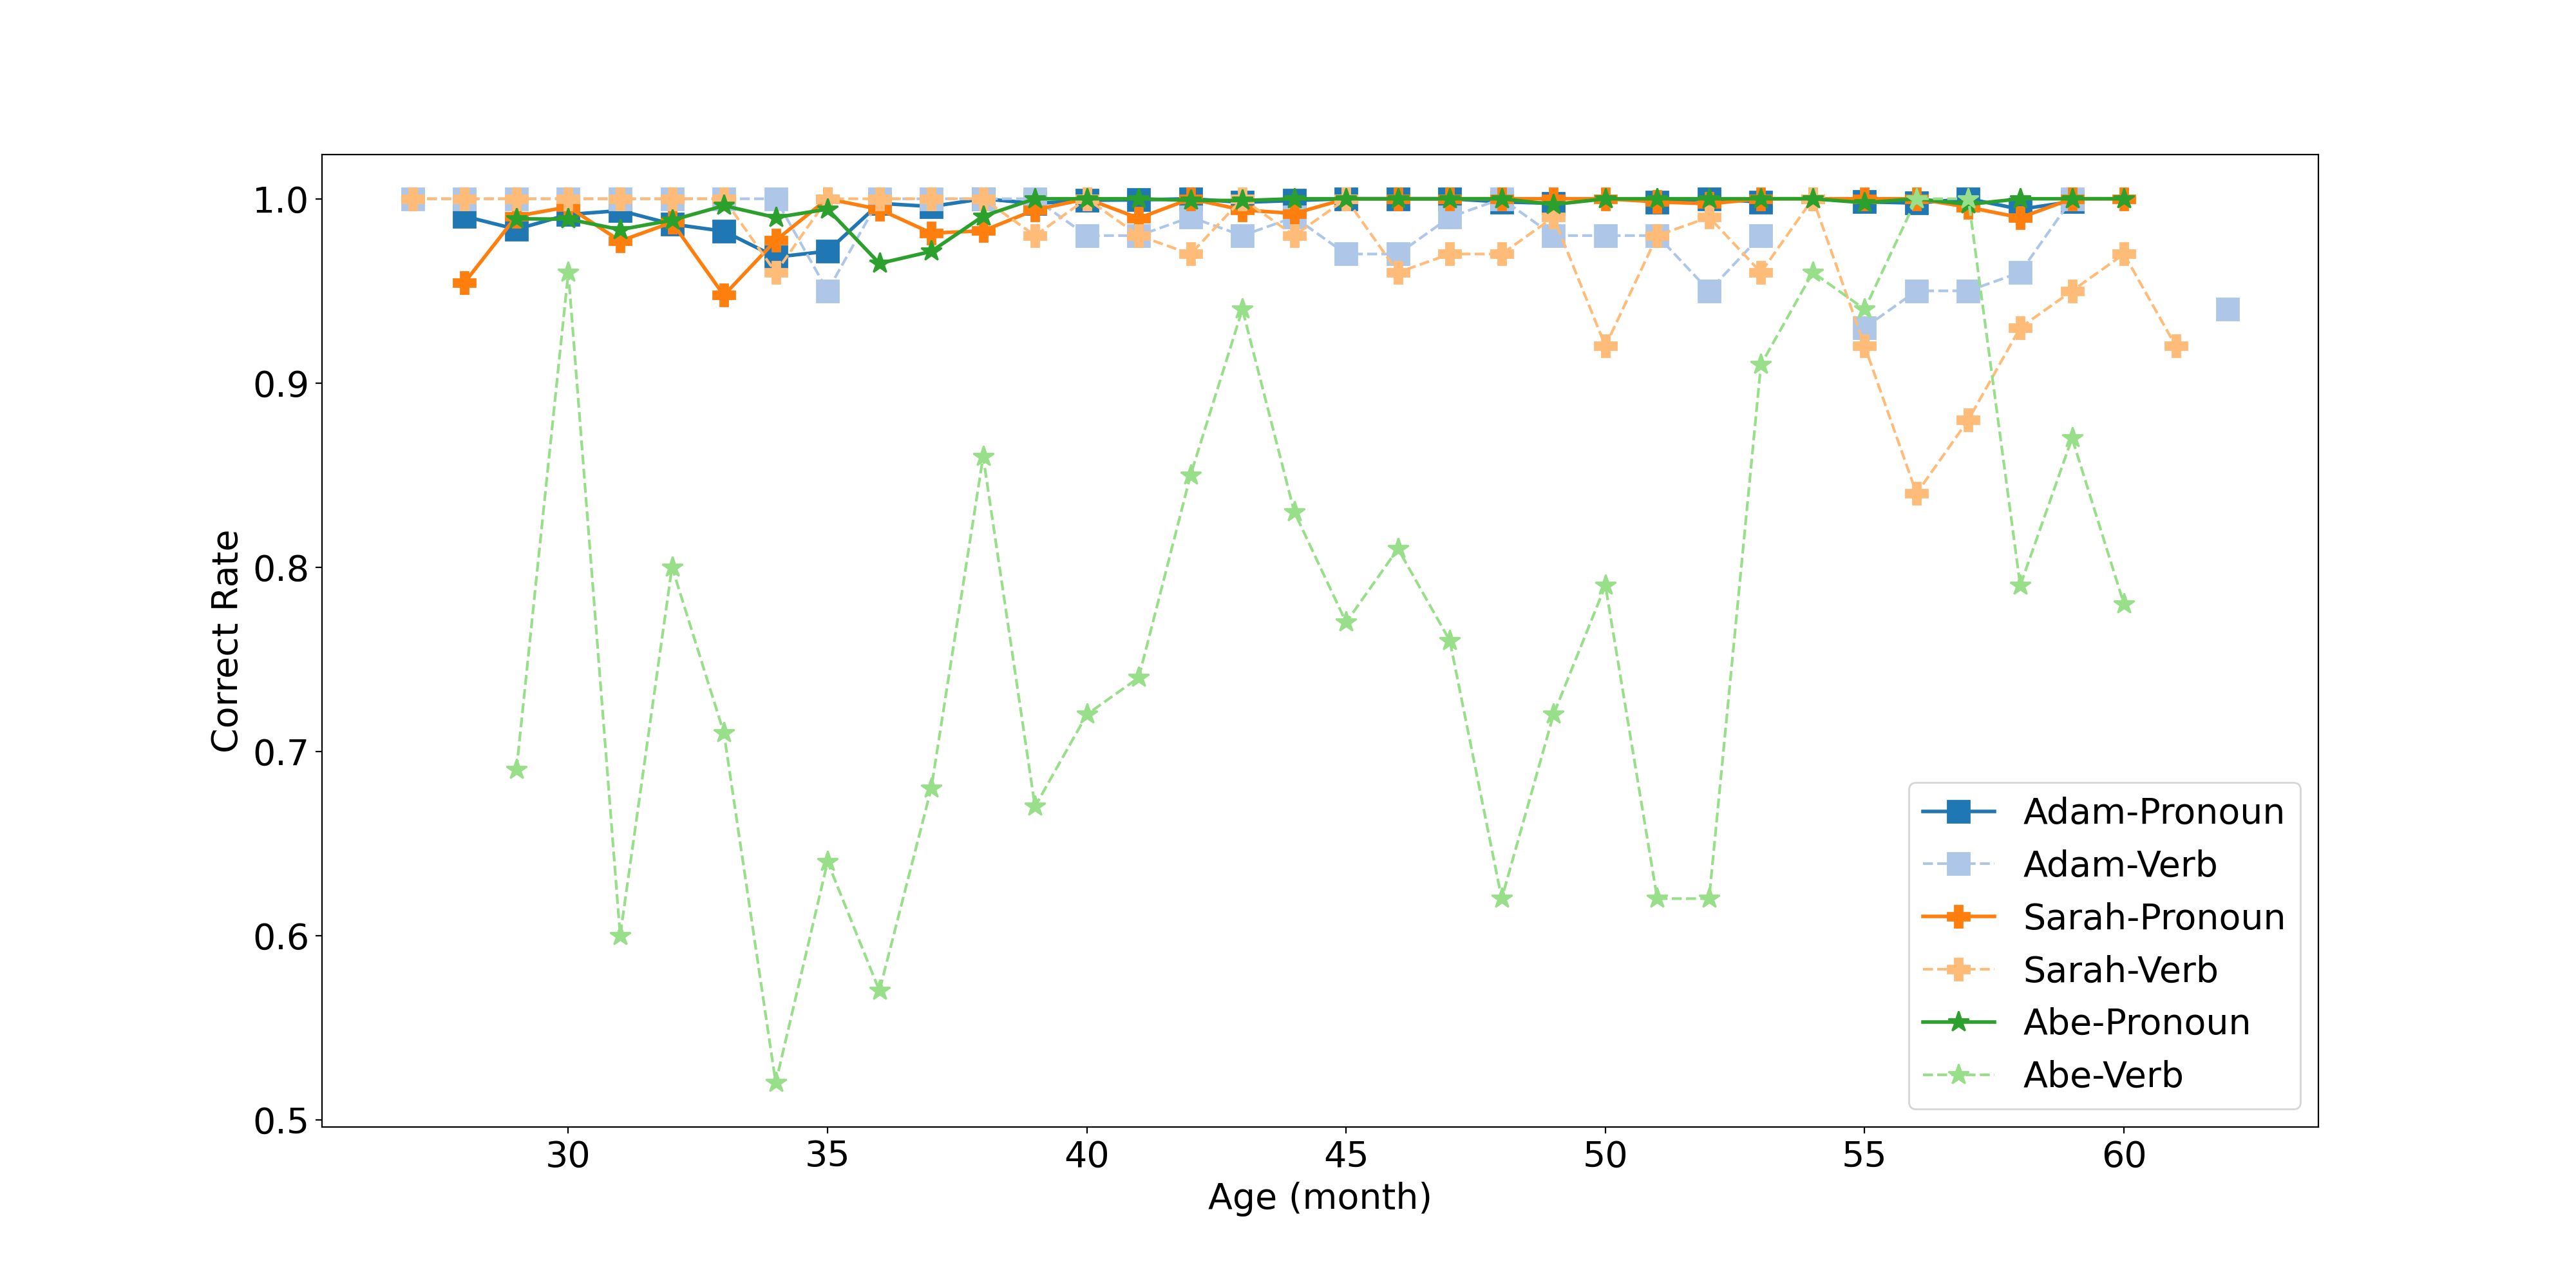
\includegraphics[scale = 0.35, width = \linewidth]{graph/AgeVerb.png}
\vspace{-3em}
\caption{Pronoun Correct Rate VS Verb Correct Rate for Adam, Abe and Sarah}
\label{fig:3}
\end{figure}
\FloatBarrier



\subsubsection{Different types of Pronoun Case Errors}
Children make many types of pronoun case errors as shown in previous sections. This subsection investigates the frequency of different types of pronoun case errors. The summary of pronoun case error data is shown in Table \ref{table:errordata}. 244,874 total pronouns were found in the children's longitudinal recordings. \textit{`I'},\textit{`my'} and \textit{`me'} are the most frequently used pronouns by the children; and \textit{`us'}, \textit{`their'} and \textit{`our'} are the least used pronouns. There were 3421 errors, with an average error rate of 1.39\%. There were five types of errors: nominative case used as an object (NOM for ACC), accusative case used as a subject (ACC for NOM) or a determiner (ACC for GEN), genitive case used as a subject (GEN for NOM) or an object (GEN for ACC). The most common errors occurred on pronoun \textit{`me'}, with 1579 \textit{`me'} used as \textit{`I'} and 165 \textit{`me'} used as \textit{`my'}. Seven pronouns (\textit{`I', `we', `she', `they', `his', `our'} and \textit{`their'}) have less than 10 errors. In addition, \textit{`I'} is the most commonly substituted pronoun, with 1579 \textit{`I's} being substituted by \textit{`me'} and 485 \textit{`I's} being substituted by \textit{`my'}, as shown in Column `Subs' in Table \ref{table:errordata}. `Pronoun Correct Rate by Use' in Column 6 is calculated as $1 - \displaystyle\frac{\text{Errors}}{\text{Total Tokens}}$.  For example, the correct rate by use for pronoun `I' is 1 -  $\displaystyle\frac{9}{118607} = 0.9999$. Most of the pronouns were used correctly over 95\% of the time, except for ‘me’ (91.80\%) and ‘her’ (91.14\%). `Pronoun Correct Rate by Argument Position' in Column 7 is calculated as the total argument positions (e.g. subject position, object position and determiner position) divided by the total positions that were  filled with a correct pronoun: $\displaystyle\frac{\text{Positions with correct pronoun}}{\text{Total argument positions}}$.  For example, for the subject position that requires a first person singular pronoun, the correct pronoun `\textit{I}' filled 118598 subject position, incorrect pronoun `\textit{me}' and `\textit{my}' filled 1579 and 485 subject positions respectively. Therefore, the correct rate by position for \textit{I} = $\displaystyle\frac{118607 - 9}{118607 - 9 + 1579 + 485} = 0.9829$. Most of the argument positions were filled with the correct pronoun over 98\% of the time, except for two positions: ‘she’ only filled 92.32\% of subject positions that required a third-person singular feminine pronoun and ‘their’ only filled 89.70\% of determiner positions that required a third-person plural pronoun. 

In addition, different types of errors are not equally popular among children. Children's errors are concentrated in three types of ACC for NOM errors: 41 children made `me-for-I' errors; 36 children made `them-for-they' errors and 30 children made `her-for-she' errors. Four types of errors (`she-for-her', `we-for-us', `they-for-them' and `our-for-we') had less than 5 children that made errors. Children don't make the same amount of errors on different error types. For some error types, children usually make that error once or twice. For example for `she-for-her' error, the maximum number of errors per child is 1 and there were 4 children who made such an error, meaning that each child only made the `she-for-her' error once. For other types of errors, there might be one or two children's errors accounted for a majority of the error tokens. For example, of total 1579 `me-for-I' errors, 858 errors were made by one child. 
 
\FloatBarrier
\begin{table}[h]
\footnotesize
\caption{Summary of Pronoun Case Error Data}
\label{table:errordata}
\begin{tabular}{c|cccccccc}
\hline
Pronoun & Tokens & Error Type & Errors & Subs & \begin{tabular}[c]{@{}l@{}}Pronoun\\ Correct\\ Rate by \\ Use\textsuperscript{a}\end{tabular} & \begin{tabular}[c]{@{}l@{}}Pronoun \\ Correct\\ Rate by\\ Argument\\ Position\textsuperscript{b}\end{tabular} & \begin{tabular}[c]{@{}l@{}}N children\\ making error\end{tabular} & \begin{tabular}[c]{@{}l@{}}Maximum\\ error/child\end{tabular} \\ \hline
I & 118607 & I-for-me & 9 & 2064 & 99.99\% & 98.29\% & 6 & 3 \\
he & 16966 & he-for-him & 27 & 157 & 99.84\% & 99.08\% & 14 & 8 \\
she & 4955 & she-for-her & 4 & 412 & 99.92\% & 92.32\% & 4 & 1 \\
we & 13525 & we-for-us & 4 & 14 & 99.97\% & 99.90\% & 3 & 2 \\
they & 9703 & they-for-them & 4 & 202 & 99.96\% & 97.96\% & 4 & 1 \\
me & 21280 & me-for-I & 1579 & 40 & \multirow{2}{*}{91.80\%} & \multirow{2}{*}{99.81\%} & 41 & 858 \\
 &  & me-for-my & 165 &  &  &  & 21 & 81 \\
him & 4732 & him-for-he & 148 & 27 & \multirow{2}{*}{95.79\%} & \multirow{2}{*}{99.24\%} & 26 & 26 \\
 &  & him-for-his & 51 &  &  &  & 11 & 30 \\
her & 4650 & her-for-she & 412 & 4 & 91.14\% & 99.94\% & 30 & 169 \\
us & 727 & us-for-we & 13 & 4 & 98.21\% & 99.73\% & 9 & 3 \\
them & 7181 & them-for-they & 194 & 4 & \multirow{2}{*}{95.95\%} & \multirow{2}{*}{99.94\%} & 36 & 42 \\
 &  & them-for-their & 97 &  &  &  & 23 & 17 \\
my & 35329 & my-for-I & 485 & 165 & \multirow{2}{*}{98.54\%} & 99.54\% & 25 & 124 \\
 &  & my-for-me & 31 &  &  &  & 7 & 8 \\
his & 5109 & his-for-he & 9 & 51 & 99.82\% & 99.01\% & 9 & 1 \\
our & 1265 & our-for-we & 1 & 0 & 99.92\% & 100.00\% & 1 & 1 \\
their & 845 & their-for-they & 8 & 97 & 99.05\% & 89.70\% & 6 & 2\\
\hline
\end{tabular}
\end{table}
\FloatBarrier

Why are children's pronoun case errors concentrated in few types of errors such as `\textit{me}-for-\textit{I}' and `\textit{her}-for-\textit{she}'? One possible explanation is that the error rate is related to how often children use a certain pronoun or how often children hear a certain pronoun in the parents' input. A Spearman's test shows that for each pronoun, there is a strong positive correlation between children's pronoun production and parents' pronoun input ($r_s$ = 0.80**, p <0.001), but there is no significant correlation between pronoun correct rate by use and children's pronoun production ($r_s$ = 0.22, p = 0.45) or parents' pronoun input ($r_s$ = 0.43, p = 0.13). Similarly, pronoun correct rate by position is not correlated with children's pronoun production ($r_s$ = -0.09, p = 0.77), or with parents' pronoun input ($r_s$ = -0.07, p = 0.81). Figure \ref{fig:corrct} visualizes that pronoun correct rate by rate and by position are not proportional to children's pronoun production or parents' input. In addition, each pronoun's error tokens are not correlated with children's pronoun production ($r_s$ = 0.30, p = 0.30) or with parents' pronoun input ($r_s$ = -0.01, p = 0.96). The results indicate that children do not produce more errors on a pronoun simply because they use that pronoun or hear that pronoun more often. Instead, children's pronoun production could be related to pronoun case errors in another way: the more often children use a pronoun, the more likely that pronoun is to be substituted. For example, \textit{`I'} is the most used pronoun by children. There were only 9 \textit{`I'}-for-\textit{'me'} errors, whereas 2064 \textit{`I'}s were substituted with \textit{`me'} and \textit{'my'}. A Spearman's test shows that children's pronoun production is positively correlated with pronouns' substituted tokens ($r_s$ = 0.56*, p = 0.03). The substituted tokens are not correlated with parents' pronoun input ($r_s$ = 0.47, p = 0.09). Figure \ref{fig:errortoken} shows that the error tokens are not correlated with children's and parents' pronoun tokens, and substituted tokens are correlated with children's pronoun production.


\FloatBarrier
\begin{figure}[!h]
    \centering
    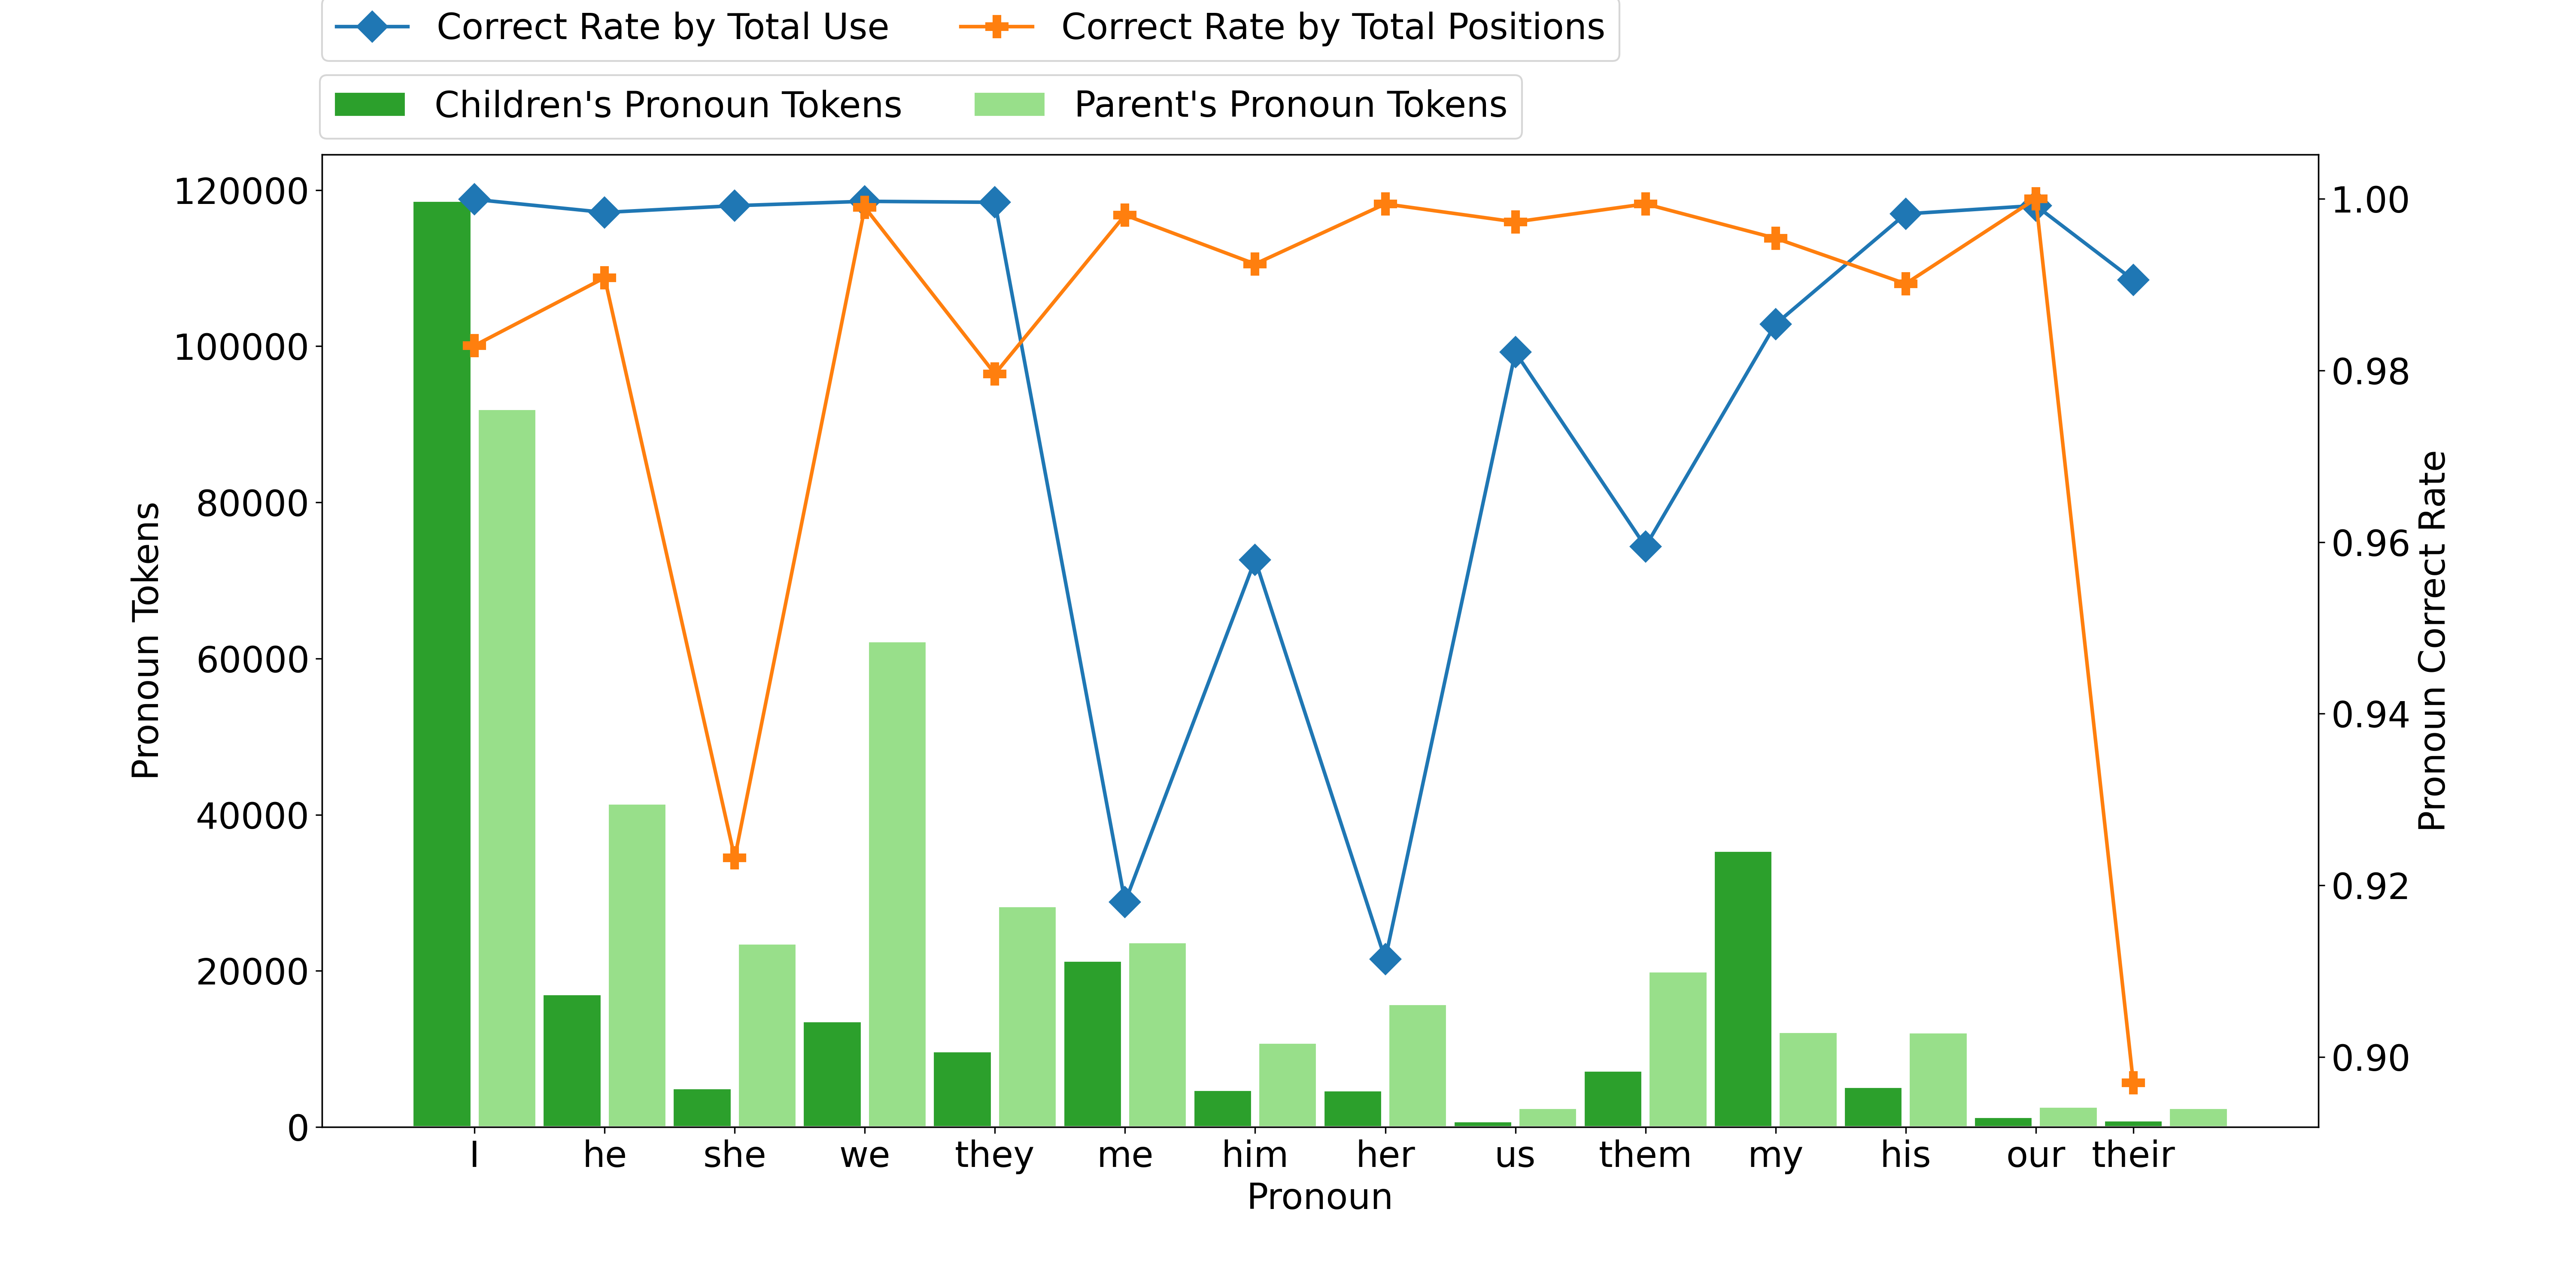
\includegraphics[scale = 0.35]{graph/PronounandRate.png}
    \vspace{-2em}
    \caption{Pronoun Correct Rate by Use and by Token, and Pronoun Tokens by Parents and Children }
    \label{fig:corrct}
\end{figure}
\FloatBarrier
\FloatBarrier
\begin{figure}[!h]
    \centering
    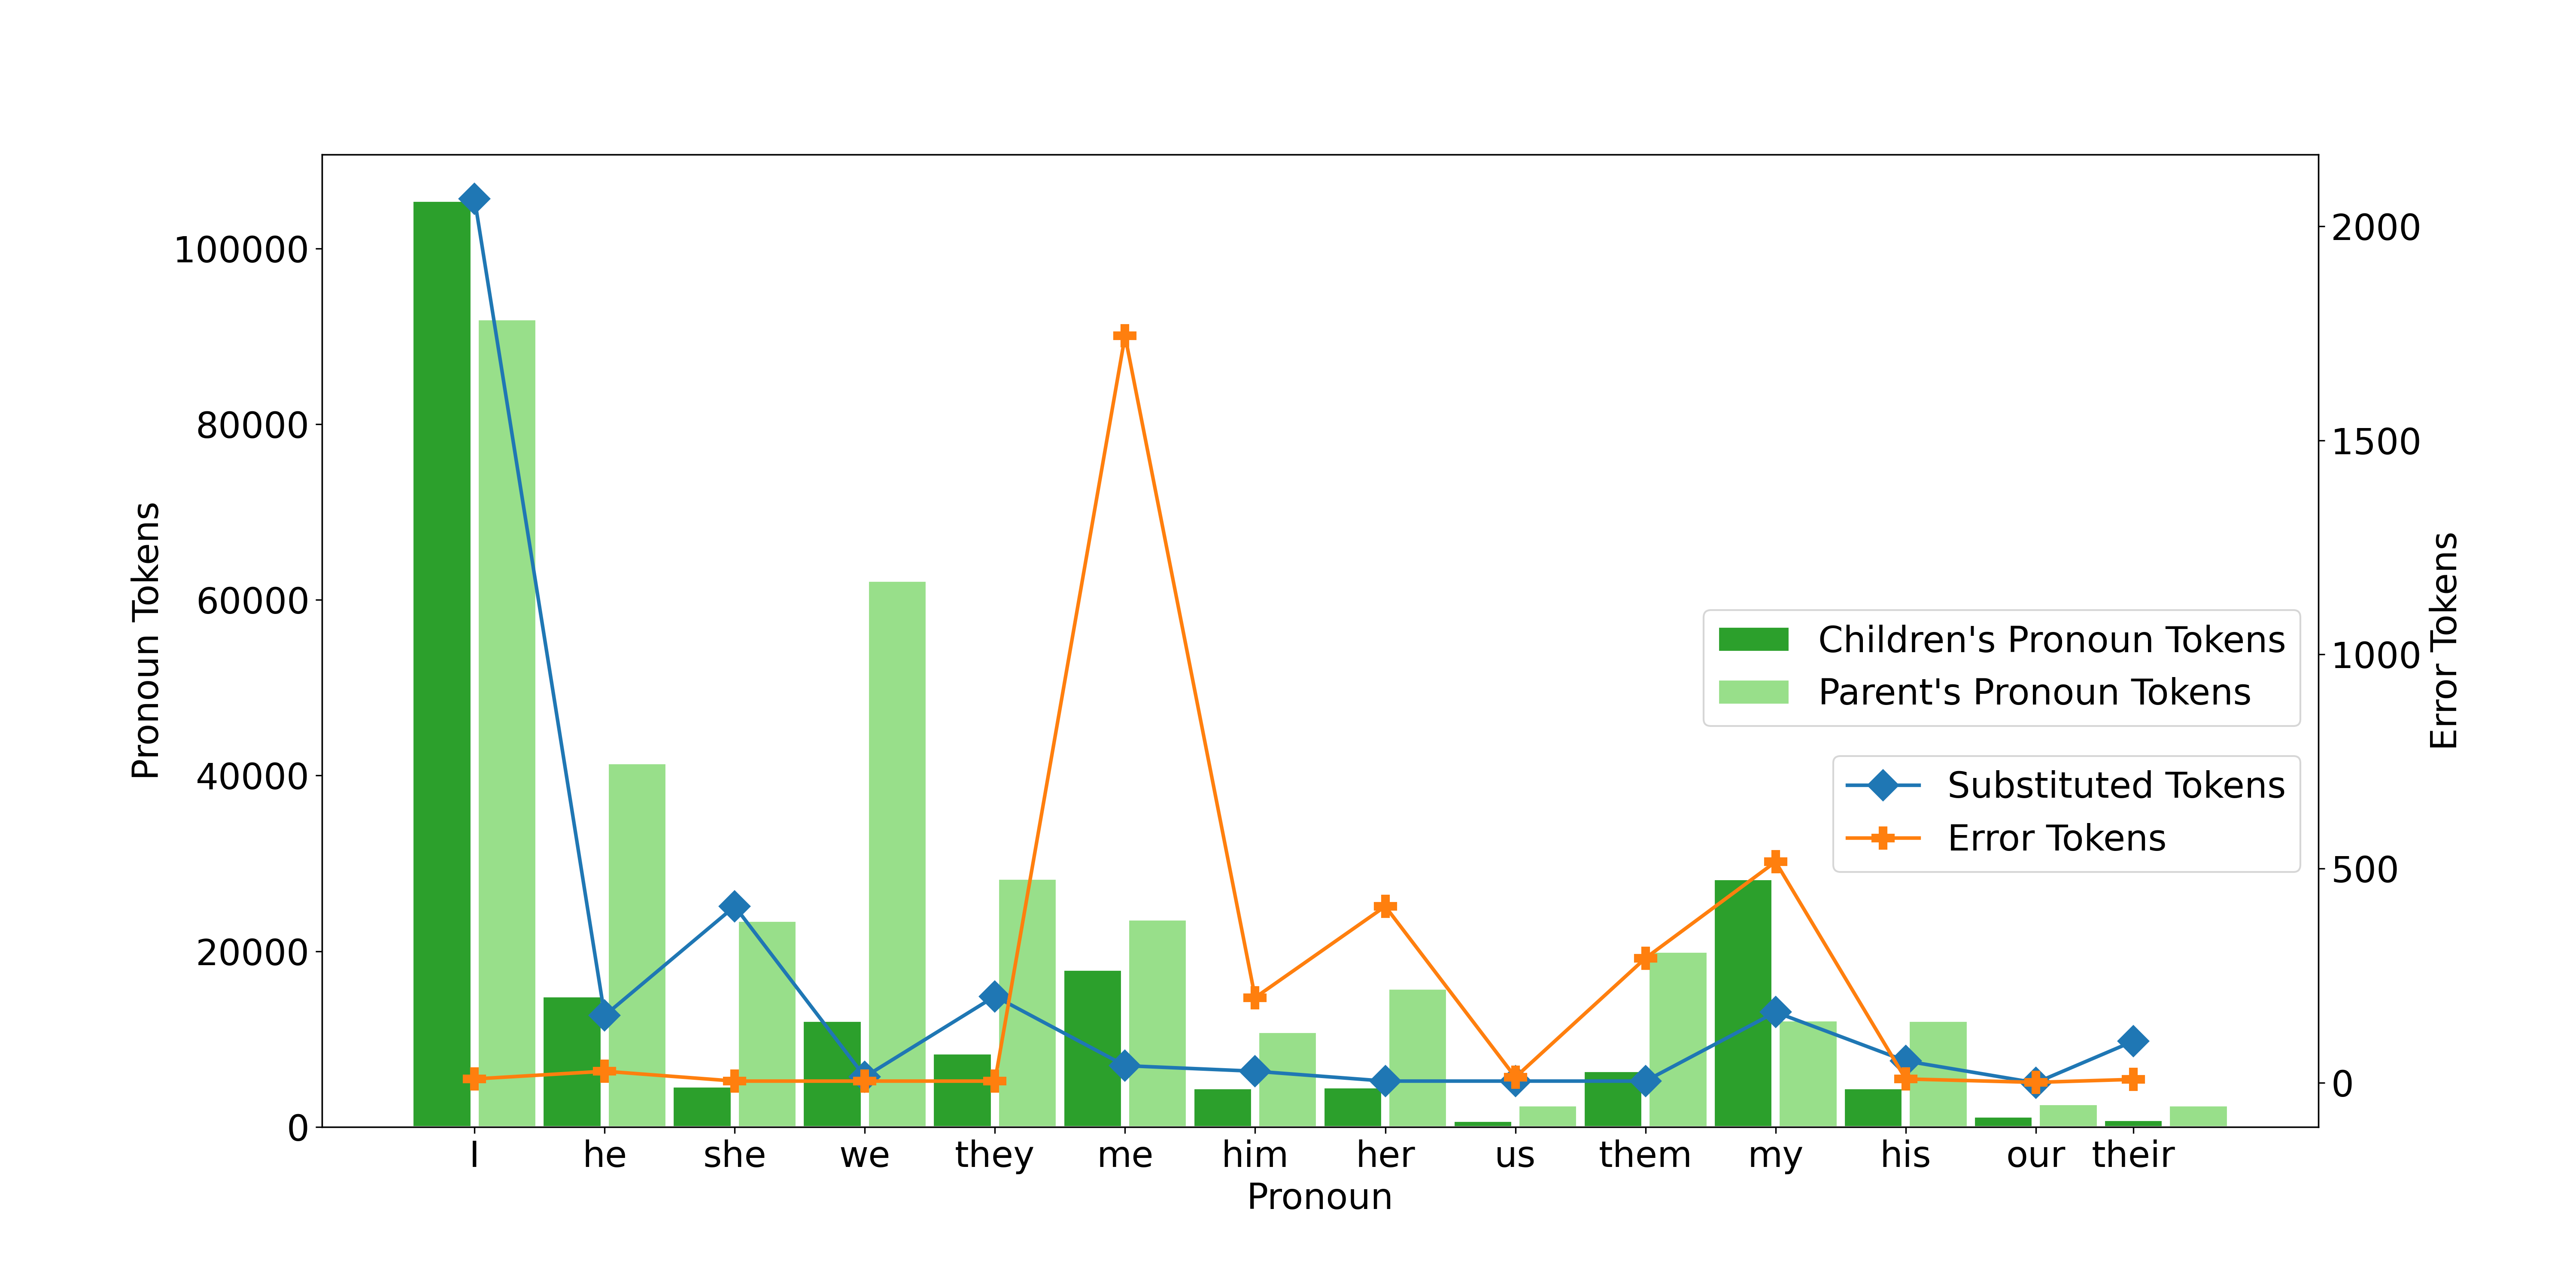
\includegraphics[scale = 0.35]{graph/Pronounandtoken.png}
    \vspace{-2em}
    \caption{Error tokens and Substituted tokens, and Pronoun tokens by Parents and Children}
    \label{fig:errortoken}
\end{figure}
\FloatBarrier


\subsection{Conclusion}
This section analyzed pronoun case errors' frequencies and patterns. First, pronoun case error is a relatively uncommon phenomenon, as most of the children rarely make any errors. 141 children in the cross-sectional data didn't make any errors, and 32 children with longitudinal recordings have less than a 1\% error rate. The average pronoun case error rate is also extremely low, with an average 1.16\% error rate for the cross-sectional data and 1.56\% for the longitudinal data. 

The pronoun case error rate has a non-monotonic relationship with children's age and mlu. The pronoun correct rate displays a U-shaped developmental pattern that children start with almost 100\% correct rate and decline to around 97\% and rise back to almost 100\% at around 5 years old. However, the correct rates at different age groups are not significantly different from each other. Since the error rate is so low during the U-shaped developmental sequences, it is difficult to judge if the changes in the correct rate are meaningful. 

Children's pronoun production and parents' pronoun input are not correlated with pronoun corrert rate or pronoun error tokens. The substituted tokens are correlated with children's pronoun production, suggesting that the more children use a pronoun, the more often that pronoun is replaced by an incorrect pronoun. 


\newpage
%\section{Study 2. Can Children's Verbal Use Explain Pronoun Case Errors? }
\subsection{ATOM Model}
Researchers have provided a wide range of explanations for pronoun case errors. From a theoretical perspective, pronoun case errors occur when the children fail to check both tense and agreement in their utterances according the to Agreement/Tense Omission Model (\textsc{atom}) \citep{wexler1998,wexler1998}. They argue that children clearly know the case system at an early age. However, children experience an Optional Infinitive stage \citep{wexler1994}, during which children produce utterances omitting inflections and with fully inflected forms at the same time. Although the theory didn't further explain why would children knowingly omit some inflections at this stage, they do believe that the errors in pronoun case in children's utterances don't reflect their impaired knowledge of the case system. They observations of the data:
\begin{exe}
\ex Non-NOM subject errors > NOM-ACC object errors 
\ex NOM subjects all with INFL, Non-NOM subjects - some have INFL some don'
\end{exe}

The ATOM model is built based on some crucial theoretical assumptions. First, they assume that the case manifests on pronouns is the result of structural licensing instead of morphological case marking, which makes pronoun case a syntactical problem but not a lexical problem. Second, they assume that the nominative case is assigned/licensed by the Agreement (\textsc{arg}), not Tense (\textsc{tns}). Moreover, they assume that Tense and Agreement are separated that they operate independently from each other \citep{chomsky1993minimalist}. 

Based on their assumptions, in order to produce a sentence with the correct case and verb inflections, the child needs to have knowledge of Agreement and Tense. More specifically, they understand the \textsc{tns} feature has to be realized on the verb and that the presence of inflection requires the nominative case to be assigned to the subject. \cite{wexler1994,wexler1996,wexler1998,wexler2000} argued that although young children produce many utterances without proper inflections, they do have the knowledge of Tense, because they experience an Optional Infinitive stage, during which they produce utterances omitting inflections and with fully inflected forms at the same time. Now the question is about children's knowledge of Agreement. The \textsc{+agr} feature can assign a nominative case on pronoun as well as trigger agreement on the verb and auxiliaries. 
Therefore, there are two \textsc{+agr} features (one realized on the pronoun, one realilzed on the verb) and they don't necessarily agree with each other:


There are four configuration:

\begin{table}[]
    \centering
    \caption{The Configurations of \textsc{arg} and \textsc{tns} with case}
    \begin{tabular}{llll}
    \toprule
        \textsc{arg/tns} & Case  & Examples  \\
    \hline
    Predicted to occur & & \\
         \textsc{+ arg, + tns} & \textsc{+ nom} & I'm going. He goes. She's gone. She went.\\
         \textsc{+ arg, - tns} & \textsc{+ nom}  & I going. He go. She gone. \\
         \textsc{- arg, + tns} & \textsc{- nom} & Me going. Him go. Her gone. Her went. \\
       \hline
       Predicted not to occur & & \\
       \textsc{+ arg, + tns} & 
        \bottomrule
    \end{tabular}
    \label{tab: pattern}
\end{table}






\subsection{Methods}
In \cite{schutze1996subject}, they used data of three children (Nina, Peter and Sarah) in CHILDES. They included the all the files that have non-NOM subject, which results in 31 files for Nina (1;11 - 2;5), 9 files for Peter (1;11 - 2;5) and 21 files for Sarah (2;8 - 3;1). They only counted finite and non-finite INFL forms occurring with the pronoun, thus ignoring utterances like \textit{I go} or \textit{me go}. In their study, finite verb types include auxiliary, modal, copula and past tense; null auxiliary and null copula are considered INFL. They also excluded full or partial imitations, self-repetitions, clearly rote or formulaic expressions and instances where the utterances plus the situation did not make it clear what the intended subject was. 
In the early cases of all the three children, they all have utterances demonstrating that they know that the accusative case is the default case. For example, all three children used the accusative case in the elliptical answers such as (\ref{elip}), and none of the nominative case has appeared in such environment.
\begin{exe}
\ex \label{elip} Mother: Who's going to eat with a big spoon?\\
Nina: Me!
\end{exe}
They counted all the finite verbs and non-finite verbs occurring with first person singular pronouns (\textit{I, me, my}) and third person singular pronouns (\textit{he, she, him, her}). The results of their study is shown in table\ref{tab:ATOMSchutze}. 
\begin{table}[!]
    \caption{\cite{schutze1996subject}'s data on Nina, Peter and Sarah}
    \label{tab:ATOMSchutze}
   \begin{minipage}[t]{0.5\textwidth}
    \centering
    \subcaption{Nina 1sg Finiteness VS Case}
    \begin{tabular}{@{}lll@{}}
        \toprule
         & \multicolumn{2}{c}{Verb form}\\
         \cline{2-3}
        Subject & Finite & -Finite \\
        \midrule
        I & 40 & 45 \\
        me + my & 2 & 13 \\
        \hline
        \%non-NOM & 5\% & 22\% \\
        \bottomrule
    \end{tabular}
\end{minipage}
\vspace{1ex}
\begin{minipage}[t]{0.5\textwidth}
    \centering
    \subcaption{Nina 3sg Finiteness VS Case}
    \begin{tabular}{@{}lll@{}}
        \toprule
         & \multicolumn{2}{c}{Verb form}\\
         \cline{2-3}
        Subject & Finite & -Finite \\
        \midrule
        he + she & 255 & 139 \\
        him + her & 14 & 120 \\
        \hline
        \%non-NOM & 5\% & 46\% \\
    \bottomrule
    \end{tabular}
    \end{minipage}
\vspace{1ex}
    %\caption{Nina Distribution by Verb Type}
    \begin{minipage}[t]{0.5\textwidth}
    \centering
    \subcaption{Nina 1sg Distribution by Verb Type}
    \begin{tabular}{@{}llll@{}}
        \toprule
            &\multicolumn{3}{c}{Subject Form}\\
            \cline{2-4}
        Verb form & I & me & my \\
        \midrule
        Auxiliary & 0 & 0 & 0 \\
        Modal & 28 & 0 & 0 \\
        Copula & 0 & 0 & 0 \\
        Past Tense & 12 & 0 & 2 \\
        \hline
        Null Auxiliary & 36 & 0 & 8 \\
        Null Copula & 9 & 2 & 3 \\
        \bottomrule
    \end{tabular}
\end{minipage}
\vspace{1ex}
\begin{minipage}[t]{0.5\textwidth}
    \centering
    \subcaption{Nina 3sg Distribution by Verb Type}
    \begin{tabular}{@{}lllll@{}}
        \toprule
            &\multicolumn{4}{c}{Subject Form}\\
            \cline{2-5}
        Verb form & he & him & she & her \\
        \midrule
        Main V with -s & 9 & 0 & 1 & 0 \\
        Aux with -s & 120 & 1 & 5 & 0 \\
        Modal & 9 & 0 & 0 & 3 \\
        Copula with -s & 90 & 2 & 5 & 2 \\
        Past Tense & 15 & 0 & 1 & 6 \\
        \hline
        Main V without -s & 85 & 9 & 5 & 51 \\
        Aux with -s & 19 & 0 & 1 & 11 \\
        Null Auxiliary & 17 & 1 & 0 & 24 \\
        Null Copula & 12 & 0 & 0 & 24 \\
        \bottomrule
    \end{tabular}
\end{minipage}
\vspace{1ex}
   \begin{minipage}[t]{0.5\textwidth}
    \centering
    \subcaption{Peter 1sg Finiteness VS Case}
    \begin{tabular}{@{}lll@{}}
        \toprule
         & \multicolumn{2}{c}{Verb form}\\
         \cline{2-3}
        Subject & Finite & -Finite \\
        \midrule
        I & 243 & 29 \\
        me + my & 3 & 8 \\
        \hline
        \%non-NOM & 1.2\% & 22\% \\
        \bottomrule
    \end{tabular}
\end{minipage}
\vspace{1ex}
   \begin{minipage}[t]{0.5\textwidth}
    \centering
    \subcaption{Peter 1sg Distribution by Verb Type}
    \begin{tabular}{@{}llll@{}}
        \toprule
            &\multicolumn{3}{c}{Subject Form}\\
            \cline{2-4}
        Verb form & I & me & my \\
        \midrule
        Auxiliary & 110 & 0 & 0 \\
        Modal & 54 & 0 & 0 \\
        Copula & 10 & 0 & 0 \\
        Past Tense & 69 & 2 & 1 \\
        \hline
        Null Auxiliary & 29 & 4 & 2 \\
        Null Copula & 0 & 1 & 1 \\
        \bottomrule
    \end{tabular}
\end{minipage}
\textbf{\linebreak}
\begin{minipage}[t]{0.5\textwidth}
    \centering
    \subcaption{Sarah 3sg Finiteness VS Case}
    \begin{tabular}{@{}lll@{}}
        \toprule
         & \multicolumn{2}{c}{Verb form}\\
         \cline{2-3}
        Subject & Finite & -Finite \\
        \midrule
        she & 21 & 24 \\
        her & 3 & 14 \\
        \hline
        \%non-NOM & 13\% & 37\% \\
    \bottomrule
    \end{tabular}
    \end{minipage}
\begin{minipage}[t]{0.5\textwidth}
    \centering
    \subcaption{Sarah 3sg Distribution by Verb Type}
    \begin{tabular}{@{}lll@{}}
        \toprule
            &\multicolumn{2}{c}{Subject Form}\\
            \cline{2-3}
        Verb form & she & her \\
        \midrule
        Main V with -s & 3 & 0 \\
        Aux with -s & 7 & 0 \\
        Modal & 3 & 0 \\
        Copula with -s & 1 & 0 \\
        Past Tense & 7 & 3 \\
        \hline
        Main V without -s & 9 & 10  \\
        Aux with -s & 1 & 0  \\
        Null Auxiliary & 7 & 3 \\
        Null Copula & 7 & 1  \\
        \bottomrule
    \end{tabular}
\end{minipage}
\end{table}

As shown in the table, for Nina, Peter and Sarah, their non-nominative case pronouns occur with non-finite verbs more frequent than finite verbs, which provides evidence for the ATOM hypothesis. Based on these three children's data, they also made some generalizations:
\begin{enumerate}
   \item non-nominative subjects almost never co-occur with inflection, except for occational past-tense;
\item The non-nominative subjects with past tense form is a real grammatical possibility for the child instead of a performance error
\item Nominative subjects also co-occur with verbs without inflections
\item non-nominative subjects can be both ACC and GEN for the same age roughly equal porportions, not conditioned by verb types
\item GEN subjects represent a real grammatical error 
\item Children exhibiting those errors reliably know the correct use of ACC and GEN forms 
\end{enumerate}



\subsection{My methodology}
In order to, \%gra tier is used to search for the verbs. Untensed verbs are tagged as \textit{'v'} or \textit{'v-root'}. Verbs with INFL are tagged detailely in the \% tier. Next table showed a breakdown of the verb types following each pronoun. 
Auxililaries include any tags that include \textit{'aux'}. Modals include any tags that include \textit{'mod}. Copulas include any tags that include \textit{'cop'}. Past tense verbs include verbs that have been tagged with \textit{'-PAST'}. Null Auxiliary include negation marker such as \textit{'not'}, which is tagged as \textit{'neg'}; progressive and perfective forms of the verb, which is tagged as \textit{'part'}. Null Copula include adjectives, adverbs and prepositions \footnote{The adverb \textit{'too'} is not counted.}. Nouns are not included in Null Copula because Nouns are more suitable to count for GEN errors. 
My data:
In appendix. 
    

\subsection{Challenges from \cite{pine2005testing}}
\cite{pine2005testing} argued that his testing method is flawed. The low rate of \textit{ACC + INFL} might be a false low rate beacuse it should be compared to a chi-squred expected rate instead of standing alone. \\



\newpage
\bibliography{bib}
\bibliographystyle{apalike}
\newpage

%\appendix
%\section{Appendix}
\begin{table}[]
\small
\centering
\caption{North American Corpus} 
%\begin{adjustbox}
\begin{tabular}{c|c|c|c|c|c}
\toprule
\textbf{Corpora}  & \textbf{Child}  & \textbf{Age} &
\textbf{Corpora}  & \textbf{Child}  & \textbf{Age}\\
\hline
\cite{bloom1974imitation}  & Peter   & 1;9-3;2 & \cite{suppes1974semantics} &  Nina & 2;0-3;4
\\
\cite{braunwald1971mother}  & Laura   & 1;5-4;0 & \cite{kuczaj1978children} &  Abe & 2;5-4;0 \\
\multirow{}{}{\cite{brown1973first}} & Adam & 2;3-4;0 & \cite{demetras1986working} & Trevor & 2;1-4;0\\
& Eve & 1;6-2;3 & \multirow{}{}{\cite{Weist2009}} & Ben & 2;4-3;4 \\
& Sarah & 2;3-4;0 & &Emily & 2;6-3;4\\
\cite{demetras1989changes} & Jimmy & 2;2-2;10 & & Emma & 2;7-3;9\\
\cite{clark1978awareness} & Shem & 2;3-3;2 &  & Jilian & 2;1-2;10\\
\cite{sachs1983talking}& Naomi & 1;3-4;9 & & Matt & 2;5-5;0\\
\cite{macwhinney2014childes} & Ross & 1;4-5;0 & & Roman & 2;3-4;0\\
\multirow{}{}{\cite{post1993language}}& She & 1;8-2;5 & \cite{Snow1990child} & Nathaniel & 3;1-3;3\\
&Tow&1;9-2;5&\cite{hayes1988vocabulary}&Geraldine&1;6-2;2\\
\hline
\hline
& \textbf{No.} & \textbf{Mean Age} & & \textbf{No.} & \textbf{Mean Age}\\
\cite{bates1991first}  & 11  & 2;4 &
\cite{bohannon1977children}  & 2 & 3;6\\
\cite{gleason1980acquisition}&19&4;8&\cite{snow1995shell}&79&3;11\\
\cite{snow1989imitativeness}&25&2;8&\cite{valian1991syntactic}&17&2;5\\
\cite{van1980effects}&19&3;9\\
\bottomrule
\end{tabular}
%\end{adjustbox}
\end{table}
\begin{table}[!]
\small
\centering
\caption{UK Corpus} 
%\begin{adjustbox}
\begin{tabular}{c|c|c|c|c|c}
\toprule
\textbf{Corpora}  & \textbf{Child}  & \textbf{Age} &
\textbf{Corpora}  & \textbf{Child}  & \textbf{Age}\\
\hline
\multirow{}{}{\cite{henry1995belfast}} & Barbara & 2;4-4;1 & \multirow{}{}{\cite{theakston2001}} & Anne & 1;10-2;9\\
& Michelle & 2;4-4;4 & & Warren& 1;10-2;9 \\
& Courtney & 3;4-4;0 & &Aran & 1;11-2;10\\
 & Rachel & 2;5-3;2 & & Becky & 2;0-2;11\\
 & Conor & 3;8-4;5 &  & Carl & 1;8-2;8\\
& Stuart & 3;5-4;5 & & Dominic & 1;10-2;10\\
 & Johnny & 3;5-4;4 & & Gail & 1;11-2;11\\
 & David & 2;0-4;2 &  & Joel & 1;11-2;10\\
\cite{rowland2006effect} & Lara & 1;9-3;3&  & John &1;11-2;10 \\
\cite{maslen2004dense} & Thomas & 2;0-4;11 & & Liz& 1;11-2;10\\
\multirow{}{}{\cite{lieven2009two}} &Eleanor &2;0-3;1 & & Nicole& 2;0-3;0 \\
&Fraser &2;0-3;0 & & Ruth& 1;11-2;11 \\
\hline
\hline
&\textbf{No.}&\textbf{Mean Age}& &\textbf{No.}&\textbf{Mean Age}\\
\cite{tommerdahl2013analyzing}&23&2;9&\cite{howe1981acquiring}&16&2;0\\
\bottomrule
\end{tabular}
%\end{adjustbox}
\end{table}


\begin{table}[]
\small
\begin{tabular}{llllllll}
name & age range & mlu range &  words & input  & pronouns & input pronouns & errors \\
\toprule
Peter & NAN & MAN & NAN & NAN & 7877 & 2384 & 155 \\
Laura & 1;5 - 7;0 & 1.0 – 6.62 & 70071 & 91822 & 10115 & 12488 & 213 \\
Adam & 2;3 - 5;2 & 2.40 – 6.46 & 175835 & 92439 & 24075 & 13235 & 589 \\
Eve & 1;6 - 2;3 & 2.09 – 4.95 & 34611 & 42601 & 4283 & 6061 & 98 \\
Sarah & 2;3 - 5;1 & 1.59 – 7.77 & 108047 & 124115 & 15472 & 16361 & 361 \\
Jimmy & 2;2 - 2;10 & 3.51 – 5.91 & 23615 & 30696 & 2761 & 2027 & 85 \\
Shem & 2;3 - 3;2 & 4.32 – 12.23 & 83536 & 10535 & 9217 & 1337 & 102 \\
Naomi & 1;3 - 4;9 & 1.30 – 7.92 & 44111 & 36079 & 5243 & 4428 & 119 \\
Ross & 0;1 - 7;8 & 1.71 - 21.0 & 165856 & 32325 & 24740 & 4944 & 397 \\
She & 1;8 - 2;5 & 2.23 - 3.55 & 6768 & 17922 & 761 & 2365 & 34 \\
Tow & 1;7 - 2;5 & 1.87 – 5.07 & 7686 & 30966 & 979 & 3871 & 64 \\
Nina & 2;0 - 3;4 & 2.25 - 6.07 & 101191 & 179999 & 11868 & 25710 & 1067 \\
Abe & 2;5 - 5;0 & 3.68 - 10.54 & 160930 & 52828 & 24820 & 8055 & 340 \\
Trevor & 2;1 - 4;0 & 4.26 – 8.04 & 26260 & 35618 & 2893 & 0 & 76 \\
Ben & 2;4 - 3;4 & 4.95 - 6.90 & 13730 & 9204 & 1638 & 1177 & 79 \\
Emily & 2;6 - 4;6 & 4.64 – 9.38 & 32325 & 1017 & 5109 & 143 & 111 \\
Emma & 2;7 - 4;8 & 3.69 – 6.40 & 26829 & 4865 & 3473 & 697 & 70 \\
Jillian & 2;1 - 2;10 & 2.77 - 7.08 & 20492 & 20226 & 2675 & 2756 & 123 \\
Matt & 2;3 - 5;0 & 2.85 - 11.09 & 46086 & 135852 & 6620 & 19669 & 101 \\
Roman & 2;3 - 4;8 & 2.98 - 11.97 & 50432 & 8848 & 6088 & 1147 & 110 \\
Nathaniel & 2;6 - 3;9 & 1.84 – 6.59 & 66036 & 121136 & 2197 & 8974 & NAN \\
Geraldine & 1;6 - 2;5 & 1.35 - 5.48 & 4564 & 16153 & 602 & 1935 & NAN \\
Anne & 1;10 - 2;9 & 1.75 - 4.15 & 50091 & 140284 & 5034 & 18766 & NAN \\
Aran & 1;11 - 2;11 & 1.46 - 5.02 & 48164 & 187083 & 7025 & 27203 & 28 \\
Barbara & 2;4 - 4;2 & 3.37 - 6.47 & 10153 & 31814 & 1354 & 5055 & 3 \\
Becky & 2;0 - 2;11 & 1.53 - 3.97 & 60488 & 97579 & 7149 & 14603 & 57 \\
Carl & 1;9 - 2;8 & 2.22 - 4.36 & 67072 & 85844 & 5513 & 10382 & 37 \\
Conor & 3;8 - 4;6 & 1.87 - 5.71 & 14832 & 52355 & 2005 & 8063 & 18 \\
Courtney & 3;4 - 4;0 & 5.13 - 6.68 & 10228 & 12036 & 1403 & 1713 & 12 \\
David & 2;0 - 4;2 & 2.32 - 6.41 & 7890 & 19966 & 1021 & 3223 & 1 \\
Dominic & 1;11 - 2;11 & 1.34 - 4.08 & 49987 & 129557 & 4969 & 18603 & 134 \\
Eleanor & 2;0 - 3;1 & 2.12 - 4.26 & 221678 & 361497 & 29191 & 48309 & 167 \\
Gail & 2;0 - 2;11 & 1.87 - 4.33 & 42233 & 104419 & 4764 & 16074 & 96 \\
Joel & 1;11 - 2;10 & 1.41 - 3.92 & 45679 & 109337 & 4984 & 15246 & 35 \\
John & 1;11 - 2;11 & 1.92 - 3.78 & 30502 & 80120 & 2181 & 10299 & 15 \\
Johnny & 3;6 - 4;4 & 3.93 - 4.52 & 6540 & 3528 & 877 & 508 & 7 \\
Lara & 1;9 - 3;4 & 1.85 - 8.0 & 175782 & 291534 & 25442 & 41210 & 188 \\
Liz & 1;11 - 2;11 & 1.52 - 4.79 & 40780 & 77560 & 5192 & 10762 & 51 \\
Michelle & 2;5 - 4;5 & 3.0 - 6.87 & 14794 & 24786 & 2401 & 3741 & 25 \\
Nicole & 2;1 - 3;0 & 1.26 - 3.61 & 36425 & 120479 & 2365 & 17915 & 38 \\
Rachel & 2;6 - 3;2 & 2.8 - 6.33 & 5932 & 20352 & 665 & 2759 & 19 \\
Ruth & 1;11 - 3;0 & 1.63 - 4.34 & 42724 & 138906 & 4129 & 19743 & 75 \\
Stuart & 3;5 - 4;5 & 4.51 - 6.34 & 16678 & 16085 & 2372 & 2403 & 27 \\
Thomas & 2;0 - 5;0 & 1.56 - 6.92 & 554257 & 1823256 & 48563 & 227178 & 410 \\
Warren & 1;10 - 2;10 & 2.02 - 4.71 & 49155 & 118113 & 4071 & 14859 & 116
\end{tabular}
\end{table}
%%%Anne
\begin{table}[]
    \caption{Anne ATOM Model}
\begin{minipage}{0.5\textwidth}
    \centering
    \subcaption{1sg Finiteness Versus Case}
    \begin{tabular}{@{}lll@{}}
        \toprule
         &\multicolumn{2}{c}{Verb form}\\
         \cline{2-3}
        Subject & Finite & -Finite \\
        \midrule
        I & 346 & 45 \\
        me + my & 5 & 78 \\
        \hline
        \%non-NOM & 1\% & 63\% \\
        \bottomrule
    \end{tabular}
\end{minipage}
\begin{minipage}{0.5\textwidth}
    \centering
    \subcaption{3sg Finiteness Versus Case}
    \begin{tabular}{@{}lll@{}}
        \toprule
         &\multicolumn{2}{c}{Verb form}\\
         \cline{2-3}
        Subject & Finite & -Finite \\
        \midrule
        he + she & 133 & 78 \\
        him + her & 8 & 36 \\
        \hline
        \%non-NOM & 6\% & 32\% \\
        \bottomrule
    \end{tabular}
    \end{minipage}
\begin{minipage}{0.5\textwidth}
    \subcaption{1sg Distribution by Verb type}
        \centering
    \begin{tabular}{@{}llll@{}}
        \toprule
            &\multicolumn{3}{c}{Subject Form}\\
            \cline{2-4}
        Verb Form & I & me & my \\
        \midrule
        Auxiliary & 25 & 0 & 0 \\
        Modal & 188 & 1 & 1 \\
        Copula & 14 & 1 & 0 \\
        Past Tense & 119 & 2 & 0 \\
        \hline
        Null Auxiliary & 31 & 6 & 13 \\
        Null Copula & 14 & 39 & 20 \\
        \bottomrule
    \end{tabular}
\end{minipage}
\begin{minipage}{0.5\textwidth}
    \subcaption{3sg pronoun}
        \centering
    \begin{tabular}{@{}lllll@{}}
        \toprule
            &\multicolumn{4}{c}{Subject Form}\\
            \cline{2-5}
        Verb form & he & him & she & her \\
        \midrule
        Main V with -s & 27 & 0 & 1 & 3 \\
        Aux with -s & 7 & 0 & 0 & 0 \\
        Modal & 29 & 1 & 5 & 0 \\
        Copula with -s & 19 & 0 & 0 & 1 \\
        Past Tense & 33 & 1 & 12 & 2 \\
        \hline
        Main V without -s & 22 & 3 & 4 & 3 \\
        Aux with -s & 2 & 0 & 1 & 0 \\
        Null Auxiliary & 28 & 0 & 6 & 3 \\
        Null Copula & 6 & 23 & 9 & 4 \\
        \bottomrule
    \end{tabular}
    \end{minipage}
\end{table}
%%%Aran
\begin{table}[]
    \caption{Aran ATOM Model}
\begin{minipage}{0.5\textwidth}
    \centering
    \subcaption{1sg Finiteness Versus Case}
    \begin{tabular}{@{}lll@{}}
        \toprule
         &\multicolumn{2}{c}{Verb form}\\
         \cline{2-3}
        Subject & Finite & -Finite \\
        \midrule
        I & 774 & 69 \\
        me + my & 5 & 72 \\
        \hline
        \%non-NOM & 1\% & 51\% \\
        \bottomrule
    \end{tabular}
\end{minipage}
\begin{minipage}{0.5\textwidth}
    \centering
    \subcaption{3sg Finiteness Versus Case}
    \begin{tabular}{@{}lll@{}}
        \toprule
         &\multicolumn{2}{c}{Verb form}\\
         \cline{2-3}
        Subject & Finite & -Finite \\
        \midrule
        he + she & 197 & 102 \\
        him + her & 0 & 43 \\
        \hline
        \%non-NOM & 0\% & 30\% \\
        \bottomrule
    \end{tabular}
    \end{minipage}
    \begin{minipage}{0.5\textwidth}
    \centering
    \subcaption{1sg Distribution by Verb type}
    \begin{tabular}{@{}llll@{}}
        \toprule
            &\multicolumn{3}{l}{Subject Form}\\
            \cline{2-4}
        Verb Form & I & me & my \\
        \midrule
        Auxiliary & 26 & 0 & 0 \\
        Modal & 467 & 1 & 0 \\
        Copula & 25 & 0 & 0 \\
        Past Tense & 256 & 4 & 0 \\
        \hline
        Null Auxiliary & 28 & 5 & 5 \\
        Null Copula & 41 & 40 & 22 \\
        \bottomrule
    \end{tabular}
\end{minipage}
\begin{minipage}{0.5\textwidth}
    \centering
    \subcaption{3sg Distribution by Verb type}
    \begin{tabular}{@{}lllll@{}}
        \toprule
            &\multicolumn{4}{l}{Subject Form}\\
            \cline{2-5}
        Verb form & he & him & she & her \\
        \midrule
        Main V with -s & 31 & 0 & 0 & 0 \\
        Aux with -s & 3 & 0 & 0 & 0 \\
        Modal & 79 & 0 & 0 & 0 \\
        Copula with -s & 9 & 0 & 0 & 0 \\
        Past Tense & 70 & 0 & 5 & 0 \\
        \hline
        Main V without -s & 59 & 1 & 2 & 1 \\
        Aux with -s & 3 & 0 & 0 & 0 \\
        Null Auxiliary & 19 & 1 & 0 & 3 \\
        Null Copula & 19 & 33 & 0 & 4 \\
        \bottomrule
    \end{tabular}
    \end{minipage}
\end{table}
%%%Barbara
\begin{table}[]
    \caption{Barbara ATOM Model}
\begin{minipage}{0.5\textwidth}
    \centering
    \subcaption{1sg Finiteness Versus Case}
    \begin{tabular}{@{}lll@{}}
        \toprule
         &\multicolumn{2}{c}{Verb form}\\
         \cline{2-3}
        Subject & Finite & -Finite \\
        \midrule
        I & 198 & 15 \\
        me + my & 2 & 21 \\
        \hline
        \%non-NOM & 1\% & 58\% \\
        \bottomrule
    \end{tabular}
\end{minipage}
\begin{minipage}{0.5\textwidth}
    \centering
    \subcaption{3sg Finiteness Versus Case}
    \begin{tabular}{@{}lll@{}}
        \toprule
         &\multicolumn{2}{c}{Verb form}\\
         \cline{2-3}
        Subject & Finite & -Finite \\
        \midrule
        he + she & 142 & 52 \\
        him + her & 0 & 6 \\
        \hline
        \%non-NOM & 0\% & 10\% \\
        \bottomrule
    \end{tabular}
    \end{minipage}
    \begin{minipage}{0.5\textwidth}
    \centering
    \subcaption{1sg Distribution by Verb type}
    \begin{tabular}{@{}llll@{}}
        \toprule
            &\multicolumn{3}{l}{Subject Form}\\
            \cline{2-4}
        Verb form & I & me & my \\
        \midrule
        Auxiliary & 11 & 0 & 0 \\
        Modal & 100 & 2 & 0 \\
        Copula & 5 & 0 & 0 \\
        Past Tense & 82 & 0 & 0 \\
        \hline
        Null Auxiliary & 7 & 2 & 0 \\
        Null Copula & 8 & 1 & 18 \\
        \bottomrule
    \end{tabular}
\end{minipage}
\begin{minipage}{0.5\textwidth}
\centering
    \subcaption{3sg Distribution by Verb type}
    \begin{tabular}{@{}lllll@{}}
        \toprule
            &\multicolumn{4}{l}{Subject Form}\\
            \cline{2-5}
        Verb form & he & him & she & her \\
        \midrule
        Main V with -s & 12 & 0 & 18 & 0 \\
        Aux with -s & 0 & 0 & 2 & 0 \\
        Modal & 11 & 0 & 21 & 0 \\
        Copula with -s & 5 & 0 & 1 & 0 \\
        Past Tense & 32 & 0 & 40 & 0 \\
        \hline
        Main V without -s & 14 & 1 & 6 & 1 \\
        Aux with -s & 0 & 0 & 0 & 0 \\
        Null Auxiliary & 13 & 0 & 13 & 0 \\
        Null Copula & 5 & 4 & 1 & 0 \\
        \bottomrule
    \end{tabular}
    \end{minipage}
\end{table}
%%%Becky
\begin{table}[]
    \caption{Becky ATOM Model}
    \begin{minipage}{0.5\textwidth}
    \centering
    \subcaption{1sg Finiteness Versus Case}
    \begin{tabular}{@{}lll@{}}
        \toprule
         &\multicolumn{2}{c}{Verb form}\\
         \cline{2-3}
        Subject & Finite & -Finite \\
        \midrule
        I & 961 & 193 \\
        me + my & 7 & 41 \\
        \hline
        \%non-NOM & 1\% & 18\% \\
        \bottomrule
    \end{tabular}
\end{minipage}
\begin{minipage}{0.5\textwidth}
    \centering
    \subcaption{3sg Finiteness Versus Case}
    \begin{tabular}{@{}lll@{}}
        \toprule
         &\multicolumn{2}{c}{Verb form}\\
         \cline{2-3}
        Subject & Finite & -Finite \\
        \midrule
        he + she & 204 & 145 \\
        him + her & 13 & 42 \\
        \hline
        \%non-NOM & 6\% & 22\% \\
        \bottomrule
    \end{tabular}
    \end{minipage}
    \begin{minipage}{0.5\textwidth}
    \centering
    \subcaption{1sg Distribution by Verb type}
    \begin{tabular}{@{}llll@{}}
        \toprule
            &\multicolumn{3}{l}{Subject Form}\\
            \cline{2-4}
        Verb form & I & me & my \\
        \midrule
        Auxiliary & 50 & 0 & 0 \\
        Modal & 438 & 2 & 1 \\
        Copula & 41 & 2 & 0 \\
        Past Tense & 432 & 1 & 1 \\
        \hline
        Null Auxiliary & 130 & 2 & 6 \\
        Null Copula & 63 & 21 & 12 \\
        \bottomrule
    \end{tabular}
\end{minipage}
\begin{minipage}{0.5\textwidth}
    \centering
    \subcaption{3sg Distribution by Verb type}
    \begin{tabular}{@{}lllll@{}}
        \toprule
            &\multicolumn{4}{l}{Subject Form}\\
            \cline{2-5}
        Verb form & he & him & she & her \\
        \midrule
        Main V with -s & 25 & 0 & 11 & 0 \\
        Aux with -s & 11 & 0 & 0 & 5 \\
        Modal & 51 & 1 & 18 & 0 \\
        Copula with -s & 19 & 0 & 4 & 1 \\
        Past Tense & 50 & 2 & 15 & 4 \\
        \hline
        Main V without -s & 56 & 6 & 15 & 1 \\
        Aux with -s & 4 & 0 & 2 & 0 \\
        Null Auxiliary & 45 & 1 & 4 & 3 \\
        Null Copula & 16 & 28 & 3 & 3 \\
        \bottomrule
    \end{tabular}
    \end{minipage}
\end{table}
%%%Carl
\begin{table}[]
    \caption{Carl's ATOM Model}
    \begin{minipage}{0.5\textwidth}
    \centering
    \subcaption{1sg Finiteness Versus Case}
    \begin{tabular}{@{}lll@{}}
        \toprule
         &\multicolumn{2}{c}{Verb form}\\
         \cline{2-3}
        Subject & Finite & -Finite \\
        \midrule
        I & 611 & 273 \\
        me + my & 5 & 26 \\
        \hline
        \%non-NOM & 1\% & 9\% \\
        \bottomrule
    \end{tabular}
\end{minipage}
\begin{minipage}{0.5\textwidth}
    \centering
    \subcaption{3sg Finiteness Versus Case}
    \begin{tabular}{@{}lll@{}}
        \toprule
         &\multicolumn{2}{c}{Verb form}\\
         \cline{2-3}
        Subject & Finite & -Finite \\
        \midrule
        he + she & 324 & 371 \\
        him + her & 0 & 9 \\
        \hline
        \%non-NOM & 0\% & 2\% \\
        \bottomrule
    \end{tabular}
    \end{minipage}
    \begin{minipage}{0.5\textwidth}
    \centering
    \subcaption{1sg Distribution by Verb type}
    \begin{tabular}{@{}llll@{}}
        \toprule
            &\multicolumn{3}{l}{Subject Form}\\
            \cline{2-4}
        Verb form & I & me & my \\
        \midrule
        Auxiliary & 2 & 0 & 0 \\
        Modal & 351 & 0 & 0 \\
        Copula & 6 & 0 & 0 \\
        Past Tense & 252 & 3 & 2 \\
        \hline
        Null Auxiliary & 232 & 2 & 6 \\
        Null Copula & 41 & 5 & 13 \\
        \bottomrule
    \end{tabular}
\end{minipage}
\begin{minipage}{0.5\textwidth}
    \centering
    \subcaption{3sg Distribution by Verb type}
    \begin{tabular}{@{}lllll@{}}
        \toprule
            &\multicolumn{4}{l}{Subject Form}\\
            \cline{2-5}
        Verb form & he & him & she & her \\
        \midrule
        Main V with -s & 67 & 0 & 0 & 0 \\
        Aux with -s & 0 & 0 & 0 & 0 \\
        Modal & 89 & 0 & 0 & 0 \\
        Copula with -s & 9 & 0 & 0 & 0 \\
        Past Tense & 156 & 0 & 3 & 0 \\
        \hline
        Main V without -s & 228 & 0 & 4 & 0 \\
        Aux with -s & 0 & 0 & 0 & 0 \\
        Null Auxiliary & 98 & 0 & 1 & 0 \\
        Null Copula & 39 & 9 & 1 & 0 \\
        \bottomrule
    \end{tabular}
    \end{minipage}
\end{table}
%%%Conor
\begin{table}[]
    \caption{Conor ATOM Model}
    \begin{minipage}{0.5\textwidth}
    \centering
    \subcaption{1sg Finiteness Versus Case}
    \begin{tabular}{@{}lll@{}}
        \toprule
         &\multicolumn{2}{c}{Verb form}\\
         \cline{2-3}
        Subject & Finite & -Finite \\
        \midrule
        I & 215 & 27 \\
        me + my & 0 & 25 \\
        \hline
        \%non-NOM & 0\% & 48\% \\
        \bottomrule
    \end{tabular}
\end{minipage}
\begin{minipage}{0.5\textwidth}
    \centering
    \subcaption{3sg Finiteness Versus Case}
    \begin{tabular}{@{}lll@{}}
        \toprule
         &\multicolumn{2}{c}{Verb form}\\
         \cline{2-3}
        Subject & Finite & -Finite \\
        \midrule
        he + she & 210 & 34 \\
        him + her & 0 & 27 \\
        \hline
        \%non-NOM & 0\% & 44\% \\
        \bottomrule
    \end{tabular}
    \end{minipage}
    \begin{minipage}{0.5\textwidth}
    \centering
    \subcaption{1sg Distribution by Verb type}
    \begin{tabular}{@{}llll@{}}
        \toprule
            &\multicolumn{3}{l}{Subject Form}\\
            \cline{2-4}
        Verb form & I & me & my \\
        \midrule
        Auxiliary & 14 & 0 & 0 \\
        Modal & 92 & 0 & 0 \\
        Copula & 13 & 0 & 0 \\
        Past Tense & 96 & 0 & 0 \\
        \hline
        Null Auxiliary & 13 & 5 & 0 \\
        Null Copula & 14 & 7 & 13 \\
        \bottomrule
    \end{tabular}
\end{minipage}
\begin{minipage}{0.5\textwidth}
    \centering
    \subcaption{3sg Distribution by Verb type}
    \begin{tabular}{@{}lllll@{}}
        \toprule
            &\multicolumn{4}{l}{Subject Form}\\
            \cline{2-5}
        Verb form & he & him & she & her \\
        \midrule
        Main V with -s & 62 & 0 & 7 & 0 \\
        Aux with -s & 7 & 0 & 7 & 0 \\
        Modal & 26 & 0 & 10 & 0 \\
        Copula with -s & 19 & 0 & 2 & 0 \\
        Past Tense & 50 & 0 & 20 & 0 \\
        \hline
        Main V without -s & 10 & 2 & 3 & 0 \\
        Aux with -s & 0 & 0 & 0 & 0 \\
        Null Auxiliary & 9 & 0 & 4 & 1 \\
        Null Copula & 7 & 24 & 1 & 0 \\
        \bottomrule
    \end{tabular}
    \end{minipage}
\end{table}
%%%Courtney
\begin{table}[]
    \caption{Courtney ATOM Model}
    \begin{minipage}{0.5\textwidth}
    \centering
    \subcaption{1sg Finiteness Versus Case}
    \begin{tabular}{@{}lll@{}}
        \toprule
         &\multicolumn{2}{c}{Verb form}\\
         \cline{2-3}
        Subject & Finite & -Finite \\
        \midrule
        I & 211 & 6 \\
        me + my & 0 & 20 \\
        \hline
        \%non-NOM & 0\% & 77\% \\
        \bottomrule
    \end{tabular}
\end{minipage}
\begin{minipage}{0.5\textwidth}
    \centering
    \subcaption{3sg Finiteness Versus Case}
    \begin{tabular}{@{}lll@{}}
        \toprule
         &\multicolumn{2}{c}{Verb form}\\
         \cline{2-3}
        Subject & Finite & -Finite \\
        \midrule
        he + she & 137 & 17 \\
        him + her & 3 & 25 \\
        \hline
        \%non-NOM & 2\% & 60\% \\
        \bottomrule
    \end{tabular}
    \end{minipage}
    \begin{minipage}{0.5\textwidth}
    
    \centering
    \subcaption{1sg Distribution by Verb type}
    \begin{tabular}{@{}llll@{}}
        \toprule
            &\multicolumn{3}{l}{Subject Form}\\
            \cline{2-4}
        Verb form & I & me & my \\
        \midrule
        Auxiliary & 11 & 0 & 0 \\
        Modal & 109 & 0 & 0 \\
        Copula & 2 & 0 & 0 \\
        Past Tense & 89 & 0 & 0 \\
        \hline
        Null Auxiliary & 5 & 1 & 0 \\
        Null Copula & 1 & 10 & 9 \\
        \bottomrule
    \end{tabular}
\end{minipage}
\begin{minipage}{0.5\textwidth}
    \centering
    \subcaption{3sg Distribution by Verb type}
    \begin{tabular}{@{}lllll@{}}
        \toprule
            &\multicolumn{4}{l}{Subject Form}\\
            \cline{2-5}
        Verb form & he & him & she & her \\
        \midrule
        Main V with -s & 28 & 0 & 9 & 0 \\
        Aux with -s & 0 & 0 & 4 & 0 \\
        Modal & 39 & 1 & 14 & 1 \\
        Copula with -s & 3 & 0 & 2 & 0 \\
        Past Tense & 24 & 0 & 14 & 1 \\
        \hline
        Main V without -s & 7 & 6 & 2 & 0 \\
        Aux with -s & 0 & 0 & 0 & 2 \\
        Null Auxiliary & 1 & 1 & 1 & 2 \\
        Null Copula & 3 & 13 & 3 & 1 \\
        \bottomrule
    \end{tabular}
    \end{minipage}
\end{table}
%%%David
\begin{table}[]
    \caption{David ATOM Model}
    \begin{minipage}{0.5\textwidth}
    \centering
    \subcaption{1sg Finiteness Versus Case}
    \begin{tabular}{@{}lll@{}}
        \toprule
         &\multicolumn{2}{c}{Verb form}\\
         \cline{2-3}
        Subject & Finite & -Finite \\
        \midrule
        I & 212 & 24 \\
        me + my & 1 & 8 \\
        \hline
        \%non-NOM & 0\% & 25\% \\
        \bottomrule
    \end{tabular}
\end{minipage}
\begin{minipage}{0.5\textwidth}
    \centering
    \subcaption{3sg Finiteness Versus Case}
    \begin{tabular}{@{}lll@{}}
        \toprule
         &\multicolumn{2}{c}{Verb form}\\
         \cline{2-3}
        Subject & Finite & -Finite \\
        \midrule
        he + she & 50 & 31 \\
        him + her & 0 & 1 \\
        \hline
        \%non-NOM & 0\% & 3\% \\
        \bottomrule
    \end{tabular}
    \end{minipage}
    \begin{minipage}{0.5\textwidth}
    
    \centering
    \subcaption{1sg Distribution by Verb type}
    \begin{tabular}{@{}llll@{}}
        \toprule
            &\multicolumn{3}{l}{Subject Form}\\
            \cline{2-4}
        Verb form & I & me & my \\
        \midrule
        Auxiliary & 8 & 0 & 0 \\
        Modal & 114 & 0 & 0 \\
        Copula & 9 & 0 & 0 \\
        Past Tense & 81 & 1 & 0 \\
        \hline
        Null Auxiliary & 17 & 2 & 2 \\
        Null Copula & 7 & 0 & 4 \\
        \bottomrule
    \end{tabular}
\end{minipage}
\begin{minipage}{0.5\textwidth}
    \centering
    \subcaption{3sg Distribution by Verb type}
    \begin{tabular}{@{}lllll@{}}
        \toprule
            &\multicolumn{4}{l}{Subject Form}\\
            \cline{2-5}
        Verb form & he & him & she & her \\
        \midrule
        Main V with -s & 8 & 0 & 1 & 0 \\
        Aux with -s & 0 & 0 & 0 & 0 \\
        Modal & 5 & 0 & 1 & 0 \\
        Copula with -s & 0 & 0 & 0 & 0 \\
        Past Tense & 22 & 0 & 13 & 0 \\
        \hline
        Main V without -s & 17 & 0 & 3 & 0 \\
        Aux with -s & 0 & 0 & 0 & 0 \\
        Null Auxiliary & 5 & 0 & 3 & 0 \\
        Null Copula & 2 & 1 & 1 & 0 \\
        \bottomrule
    \end{tabular}
    \end{minipage}
\end{table}

%%%Dominic
\begin{table}[]
    \caption{Dominic ATOM Model}
    \begin{minipage}{0.5\textwidth}
    \centering
    \subcaption{1sg Finiteness Versus Case}
    \begin{tabular}{@{}lll@{}}
        \toprule
         &\multicolumn{2}{c}{Verb form}\\
         \cline{2-3}
        Subject & Finite & -Finite \\
        \midrule
        I & 620 & 150 \\
        me + my & 5 & 31 \\
        \hline
        \%non-NOM & 1\% & 17\% \\
        \bottomrule
    \end{tabular}
\end{minipage}
\begin{minipage}{0.5\textwidth}
    \centering
    \subcaption{3sg Finiteness Versus Case}
    \begin{tabular}{@{}lll@{}}
        \toprule
         &\multicolumn{2}{c}{Verb form}\\
         \cline{2-3}
        Subject & Finite & -Finite \\
        \midrule
        he + she & 53 & 39 \\
        him + her & 1 & 1 \\
        \hline
        \%non-NOM & 2\% & 2\% \\
        \bottomrule
    \end{tabular}
    \end{minipage}
    \begin{minipage}{0.5\textwidth}
    \centering
    \subcaption{1sg Distribution by Verb type}
    \begin{tabular}{@{}llll@{}}
        \toprule
            &\multicolumn{3}{l}{Subject Form}\\
            \cline{2-4}
        Verb form & I & me & my \\
        \midrule
        Auxiliary & 30 & 0 & 0 \\
        Modal & 318 & 0 & 1 \\
        Copula & 44 & 0 & 0 \\
        Past Tense & 228 & 2 & 2 \\
        \hline
        Null Auxiliary & 128 & 1 & 6 \\
        Null Copula & 22 & 3 & 21 \\
        \bottomrule
    \end{tabular}
\end{minipage}
\begin{minipage}{0.5\textwidth}
    \centering
    \subcaption{3sg Distribution by Verb type}
    \begin{tabular}{@{}lllll@{}}
        \toprule
            &\multicolumn{4}{l}{Subject Form}\\
            \cline{2-5}
        Verb form & he & him & she & her \\
        \midrule
        Main V with -s & 12 & 0 & 2 & 1 \\
        Aux with -s & 5 & 0 & 0 & 0 \\
        Modal & 9 & 0 & 1 & 0 \\
        Copula with -s & 4 & 0 & 0 & 0 \\
        Past Tense & 16 & 0 & 4 & 0 \\
        \hline
        Main V without -s & 11 & 0 & 1 & 0 \\
        Aux with -s & 0 & 0 & 0 & 0 \\
        Null Auxiliary & 13 & 0 & 2 & 0 \\
        Null Copula & 11 & 1 & 1 & 0 \\
        \bottomrule
    \end{tabular}
    \end{minipage}
\end{table}
%%%Eleanor

\begin{table}[]
    \caption{Eleanor's ATOM Model}
    \begin{minipage}{0.5\textwidth}
    \centering
    \subcaption{1sg Finiteness Versus Case}
    \begin{tabular}{@{}lll@{}}
        \toprule
         &\multicolumn{2}{c}{Verb form}\\
         \cline{2-3}
        Subject & Finite & -Finite \\
        \midrule
        I & 4069 & 689 \\
        me + my & 12 & 206 \\
        \hline
        \%non-NOM & 0\% & 23\% \\
        \bottomrule
    \end{tabular}
\end{minipage}
\begin{minipage}{0.5\textwidth}
    \centering
    \subcaption{3sg Finiteness Versus Case}
    \begin{tabular}{@{}lll@{}}
        \toprule
         &\multicolumn{2}{c}{Verb form}\\
         \cline{2-3}
        Subject & Finite & -Finite \\
        \midrule
        he + she & 822 & 251 \\
        him + her & 0 & 100 \\
        \hline
        \%non-NOM & 0\% & 28\% \\
        \bottomrule
    \end{tabular}
    \end{minipage}
    \begin{minipage}{0.5\textwidth}
    
    \centering
    \subcaption{1sg Distribution by Verb type}
    \begin{tabular}{@{}llll@{}}
        \toprule
            &\multicolumn{3}{l}{Subject Form}\\
            \cline{2-4}
        Verb form & I & me & my \\
        \midrule
        Auxiliary & 137 & 0 & 0 \\
        Modal & 2475 & 2 & 0 \\
        Copula & 154 & 0 & 1 \\
        Past Tense & 1303 & 5 & 4 \\
        \hline
        Null Auxiliary & 413 & 10 & 19 \\
        Null Copula & 276 & 61 & 116 \\
        \bottomrule
    \end{tabular}
\end{minipage}
\begin{minipage}{0.5\textwidth}
    \centering
    \subcaption{3sg Distribution by Verb type}
    \begin{tabular}{@{}lllll@{}}
        \toprule
            &\multicolumn{4}{l}{Subject Form}\\
            \cline{2-5}
        Verb form & he & him & she & her \\
        \midrule
        Main V with -s & 109 & 0 & 65 & 0 \\
        Aux with -s & 20 & 0 & 12 & 0 \\
        Modal & 144 & 0 & 80 & 0 \\
        Copula with -s & 82 & 0 & 33 & 0 \\
        Past Tense & 190 & 0 & 87 & 0 \\
        \hline
        Main V without -s & 89 & 4 & 37 & 2 \\
        Aux with -s & 5 & 0 & 3 & 0 \\
        Null Auxiliary & 51 & 2 & 25 & 0 \\
        Null Copula & 30 & 80 & 11 & 12 \\
        \bottomrule
    \end{tabular}
    \end{minipage}
\end{table}
%%%Gail

\begin{table}[]
    \caption{Gail's ATOM Model}
    \begin{minipage}{0.5\textwidth}
    \centering
    \subcaption{1sg Finiteness Versus Case}
    \begin{tabular}{@{}lll@{}}
        \toprule
         &\multicolumn{2}{c}{Verb form}\\
         \cline{2-3}
        Subject & Finite & -Finite \\
        \midrule
        I & 456 & 159 \\
        me + my & 5 & 57 \\
        \hline
        \%non-NOM & 1\% & 26\% \\
        \bottomrule
    \end{tabular}
\end{minipage}
\begin{minipage}{0.5\textwidth}
    \centering
    \subcaption{3sg Finiteness Versus Case}
    \begin{tabular}{@{}lll@{}}
        \toprule
         &\multicolumn{2}{c}{Verb form}\\
         \cline{2-3}
        Subject & Finite & -Finite \\
        \midrule
        he + she & 75 & 24 \\
        him + her & 11 & 49 \\
        \hline
        \%non-NOM & 13\% & 67\% \\
        \bottomrule
    \end{tabular}
    \end{minipage}
    \begin{minipage}{0.5\textwidth}
    \centering
    \subcaption{1sg Distribution by Verb type}
    \begin{tabular}{@{}llll@{}}
        \toprule
            &\multicolumn{3}{l}{Subject Form}\\
            \cline{2-4}
        Verb form & I & me & my \\
        \midrule
        Auxiliary & 17 & 0 & 0 \\
        Modal & 241 & 1 & 0 \\
        Copula & 13 & 0 & 0 \\
        Past Tense & 185 & 0 & 4 \\
        \hline
        Null Auxiliary & 115 & 0 & 14 \\
        Null Copula & 44 & 14 & 29 \\
        \bottomrule
    \end{tabular}
\end{minipage}
\begin{minipage}{0.5\textwidth}
    \centering
    \subcaption{3sg Distribution by Verb type}
    \begin{tabular}{@{}lllll@{}}
        \toprule
            &\multicolumn{4}{l}{Subject Form}\\
            \cline{2-5}
        Verb form & he & him & she & her \\
        \midrule
        Main V with -s & 8 & 0 & 1 & 0 \\
        Aux with -s & 4 & 0 & 0 & 0 \\
        Modal & 17 & 0 & 0 & 0 \\
        Copula with -s & 12 & 0 & 2 & 0 \\
        Past Tense & 29 & 1 & 2 & 10 \\
        \hline
        Main V without -s & 12 & 4 & 0 & 7 \\
        Aux with -s & 1 & 0 & 0 & 1 \\
        Null Auxiliary & 7 & 3 & 2 & 12 \\
        Null Copula & 2 & 18 & 0 & 4 \\
        \bottomrule
    \end{tabular}
    \end{minipage}
\end{table}
%%%Joel

\begin{table}[]
    \caption{Joel's ATOM Model}
    \begin{minipage}{0.5\textwidth}
    \centering
    \subcaption{1sg Finiteness Versus Case}
    \begin{tabular}{@{}lll@{}}
        \toprule
         &\multicolumn{2}{c}{Verb form}\\
         \cline{2-3}
        Subject & Finite & -Finite \\
        \midrule
        I & 569 & 118 \\
        me + my & 2 & 45 \\
        \hline
        \%non-NOM & 0\% & 28\% \\
        \bottomrule
    \end{tabular}
\end{minipage}
\begin{minipage}{0.5\textwidth}
    \centering
    \subcaption{3sg Finiteness Versus Case}
    \begin{tabular}{@{}lll@{}}
        \toprule
         &\multicolumn{2}{c}{Verb form}\\
         \cline{2-3}
        Subject & Finite & -Finite \\
        \midrule
        he + she & 128 & 62 \\
        him + her & 1 & 40 \\
        \hline
        \%non-NOM & 1\% & 39\% \\
        \bottomrule
    \end{tabular}
    \end{minipage}
    \begin{minipage}{0.5\textwidth}
    
    \centering
    \subcaption{1sg Distribution by Verb type}
    \begin{tabular}{@{}llll@{}}
        \toprule
            &\multicolumn{3}{l}{Subject Form}\\
            \cline{2-4}
        Verb form & I & me & my \\
        \midrule
        Auxiliary & 17 & 0 & 0 \\
        Modal & 187 & 1 & 0 \\
        Copula & 31 & 0 & 0 \\
        Past Tense & 334 & 1 & 0 \\
        \hline
        Null Auxiliary & 79 & 0 & 10 \\
        Null Copula & 39 & 16 & 19 \\
        \bottomrule
    \end{tabular}
\end{minipage}
\begin{minipage}{0.5\textwidth}
    \centering
    \subcaption{3sg Distribution by Verb type}
    \begin{tabular}{@{}lllll@{}}
        \toprule
            &\multicolumn{4}{l}{Subject Form}\\
            \cline{2-5}
        Verb form & he & him & she & her \\
        \midrule
        Main V with -s & 33 & 0 & 2 & 0 \\
        Aux with -s & 0 & 0 & 0 & 0 \\
        Modal & 21 & 1 & 2 & 0 \\
        Copula with -s & 16 & 0 & 0 & 0 \\
        Past Tense & 50 & 0 & 4 & 0 \\
        \hline
        Main V without -s & 32 & 2 & 3 & 1 \\
        Aux with -s & 1 & 2 & 0 & 0 \\
        Null Auxiliary & 17 & 0 & 5 & 0 \\
        Null Copula & 4 & 35 & 0 & 0 \\
        \bottomrule
    \end{tabular}
    \end{minipage}
\end{table}
%%%John

\begin{table}[]
    \caption{John's ATOM Model}
    \begin{minipage}{0.5\textwidth}
    \centering
    \subcaption{1sg Finiteness Versus Case}
    \begin{tabular}{@{}lll@{}}
        \toprule
         &\multicolumn{2}{c}{Verb form}\\
         \cline{2-3}
        Subject & Finite & -Finite \\
        \midrule
        I & 186 & 75 \\
        me + my & 1 & 8 \\
        \hline
        \%non-NOM & 1\% & 10\% \\
        \bottomrule
    \end{tabular}
\end{minipage}
\begin{minipage}{0.5\textwidth}
    \centering
    \subcaption{3sg Finiteness Versus Case}
    \begin{tabular}{@{}lll@{}}
        \toprule
         &\multicolumn{2}{c}{Verb form}\\
         \cline{2-3}
        Subject & Finite & -Finite \\
        \midrule
        he + she & 8 & 22 \\
        him + her & 0 & 4 \\
        \hline
        \%non-NOM & 0\% & 15\% \\
        \bottomrule
    \end{tabular}
    \end{minipage}
    \begin{minipage}{0.5\textwidth}
    
    \centering
    \subcaption{1sg Distribution by Verb type}
    \begin{tabular}{@{}llll@{}}
        \toprule
            &\multicolumn{3}{l}{Subject Form}\\
            \cline{2-4}
        Verb form & I & me & my \\
        \midrule
        Auxiliary & 1 & 0 & 0 \\
        Modal & 62 & 0 & 0 \\
        Copula & 2 & 0 & 0 \\
        Past Tense & 121 & 1 & 0 \\
        \hline
        Null Auxiliary & 55 & 0 & 0 \\
        Null Copula & 20 & 2 & 6 \\
        \bottomrule
    \end{tabular}
\end{minipage}
\begin{minipage}{0.5\textwidth}
    \centering
    \subcaption{3sg Distribution by Verb type}
    \begin{tabular}{@{}lllll@{}}
        \toprule
            &\multicolumn{4}{l}{Subject Form}\\
            \cline{2-5}
        Verb form & he & him & she & her \\
        \midrule
        Main V with -s & 1 & 0 & 0 & 0 \\
        Aux with -s & 0 & 0 & 0 & 0 \\
        Modal & 0 & 0 & 0 & 0 \\
        Copula with -s & 3 & 0 & 0 & 0 \\
        Past Tense & 2 & 0 & 2 & 0 \\
        \hline
        Main V without -s & 6 & 0 & 6 & 0 \\
        Aux with -s & 0 & 0 & 0 & 0 \\
        Null Auxiliary & 4 & 0 & 4 & 0 \\
        Null Copula & 0 & 4 & 2 & 0 \\
        \bottomrule
    \end{tabular}
    \end{minipage}
\end{table}
%%%Johnny
\begin{table}[]
    \caption{Johnny ATOM Model}
    \begin{minipage}{0.5\textwidth}
    \centering
    \subcaption{1sg Finiteness Versus Case}
    \begin{tabular}{@{}lll@{}}
        \toprule
         &\multicolumn{2}{c}{Verb form}\\
         \cline{2-3}
        Subject & Finite & -Finite \\
        \midrule
        I & 138 & 6 \\
        me + my & 0 & 16 \\
        \hline
        \%non-NOM & 0\% & 73\% \\
        \bottomrule
    \end{tabular}
\end{minipage}
\begin{minipage}{0.5\textwidth}
    \centering
    \subcaption{3sg Finiteness Versus Case}
    \begin{tabular}{@{}lll@{}}
        \toprule
         &\multicolumn{2}{c}{Verb form}\\
         \cline{2-3}
        Subject & Finite & -Finite \\
        \midrule
        he + she & 52 & 12 \\
        him + her & 0 & 4 \\
        \hline
        \%non-NOM & 0\% & 25\% \\
        \bottomrule
    \end{tabular}
    \end{minipage}
    \begin{minipage}{0.5\textwidth}
    
    \centering
    \subcaption{1sg Distribution by Verb type}
    \begin{tabular}{@{}llll@{}}
        \toprule
            &\multicolumn{3}{l}{Subject Form}\\
            \cline{2-4}
        Verb form & I & me & my \\
        \midrule
        Auxiliary & 7 & 0 & 0 \\
        Modal & 62 & 0 & 0 \\
        Copula & 4 & 0 & 0 \\
        Past Tense & 65 & 0 & 0 \\
        \hline
        Null Auxiliary & 1 & 0 & 0 \\
        Null Copula & 5 & 6 & 10 \\
        \bottomrule
    \end{tabular}
\end{minipage}
\begin{minipage}{0.5\textwidth}
    \centering
    \subcaption{3sg Distribution by Verb type}
    \begin{tabular}{@{}lllll@{}}
        \toprule
            &\multicolumn{4}{l}{Subject Form}\\
            \cline{2-5}
        Verb form & he & him & she & her \\
        \midrule
        Main V with -s & 8 & 0 & 4 & 0 \\
        Aux with -s & 1 & 0 & 2 & 0 \\
        Modal & 7 & 0 & 9 & 0 \\
        Copula with -s & 4 & 0 & 0 & 0 \\
        Past Tense & 8 & 0 & 9 & 0 \\
        \hline
        Main V without -s & 5 & 0 & 2 & 0 \\
        Aux with -s & 1 & 0 & 0 & 0 \\
        Null Auxiliary & 3 & 0 & 1 & 0 \\
        Null Copula & 0 & 4 & 0 & 0 \\
        \bottomrule
    \end{tabular}
    \end{minipage}
\end{table}
%%%Lara
\begin{table}[]
    \caption{Lara ATOM Model}
    \begin{minipage}{0.5\textwidth}
    \centering
    \subcaption{1sg Finiteness Versus Case}
    \begin{tabular}{@{}lll@{}}
        \toprule
         &\multicolumn{2}{c}{Verb form}\\
         \cline{2-3}
        Subject & Finite & -Finite \\
        \midrule
        I & 2158 & 95 \\
        me + my & 10 & 261 \\
        \hline
        \%non-NOM & 0\% & 73\% \\
        \bottomrule
    \end{tabular}
\end{minipage}
\begin{minipage}{0.5\textwidth}
    \centering
    \subcaption{3sg Finiteness Versus Case}
    \begin{tabular}{@{}lll@{}}
        \toprule
         &\multicolumn{2}{c}{Verb form}\\
         \cline{2-3}
        Subject & Finite & -Finite \\
        \midrule
        he + she & 664 & 346 \\
        him + her & 3 & 63 \\
        \hline
        \%non-NOM & 0\% & 15\% \\
        \bottomrule
    \end{tabular}
    \end{minipage}
    \begin{minipage}{0.5\textwidth}
    
    \centering
    \subcaption{1sg Distribution by Verb type}
    \begin{tabular}{@{}llll@{}}
        \toprule
            &\multicolumn{3}{l}{Subject Form}\\
            \cline{2-4}
        Verb form & I & me & my \\
        \midrule
        Auxiliary & 154 & 0 & 0 \\
        Modal & 1362 & 4 & 1 \\
        Copula & 64 & 0 & 0 \\
        Past Tense & 578 & 5 & 0 \\
        \hline
        Null Auxiliary & 39 & 8 & 18 \\
        Null Copula & 56 & 87 & 148 \\
        \bottomrule
    \end{tabular}
\end{minipage}
\begin{minipage}{0.5\textwidth}
    \centering
    \subcaption{3sg Distribution by Verb type}
    \begin{tabular}{@{}lllll@{}}
        \toprule
            &\multicolumn{4}{l}{Subject Form}\\
            \cline{2-5}
        Verb form & he & him & she & her \\
        \midrule
        Main V with -s & 68 & 0 & 81 & 1 \\
        Aux with -s & 32 & 0 & 14 & 0 \\
        Modal & 85 & 0 & 135 & 2 \\
        Copula with -s & 23 & 0 & 24 & 0 \\
        Past Tense & 114 & 0 & 88 & 0 \\
        \hline
        Main V without -s & 59 & 1 & 51 & 9 \\
        Aux with -s & 16 & 0 & 7 & 2 \\
        Null Auxiliary & 97 & 0 & 72 & 5 \\
        Null Copula & 32 & 31 & 12 & 15 \\
        \bottomrule
    \end{tabular}
    \end{minipage}
\end{table}
%%%Liz
\begin{table}[]
    \caption{Liz's ATOM Model}
    \begin{minipage}{0.5\textwidth}
    \centering
    \subcaption{1sg Finiteness Versus Case}
    \begin{tabular}{@{}lll@{}}
        \toprule
         &\multicolumn{2}{c}{Verb form}\\
         \cline{2-3}
        Subject & Finite & -Finite \\
        \midrule
        I & 518 & 386 \\
        me + my & 3 & 69 \\
        \hline
        \%non-NOM & 1\% & 15\% \\
        \bottomrule
    \end{tabular}
\end{minipage}
\begin{minipage}{0.5\textwidth}
    \centering
    \subcaption{3sg Finiteness Versus Case}
    \begin{tabular}{@{}lll@{}}
        \toprule
         &\multicolumn{2}{c}{Verb form}\\
         \cline{2-3}
        Subject & Finite & -Finite \\
        \midrule
        he + she & 79 & 62 \\
        him + her & 1 & 23 \\
        \hline
        \%non-NOM & 1\% & 27\% \\
        \bottomrule
    \end{tabular}
    \end{minipage}
    \begin{minipage}{0.5\textwidth}
    
    \centering
    \subcaption{1sg Distribution by Verb type}
    \begin{tabular}{@{}llll@{}}
        \toprule
            &\multicolumn{3}{l}{Subject Form}\\
            \cline{2-4}
        Verb form & I & me & my \\
        \midrule
        Auxiliary & 17 & 0 & 0 \\
        Modal & 187 & 0 & 1 \\
        Copula & 18 & 0 & 0 \\
        Past Tense & 296 & 0 & 2 \\
        \hline
        Null Auxiliary & 296 & 2 & 15 \\
        Null Copula & 90 & 22 & 30 \\
        \bottomrule
    \end{tabular}
\end{minipage}
\begin{minipage}{0.5\textwidth}
    \centering
    \subcaption{3sg Distribution by Verb type}
    \begin{tabular}{@{}lllll@{}}
        \toprule
            &\multicolumn{4}{l}{Subject Form}\\
            \cline{2-5}
        Verb form & he & him & she & her \\
        \midrule
        Main V with -s & 4 & 0 & 1 & 0 \\
        Aux with -s & 0 & 0 & 0 & 0 \\
        Modal & 12 & 1 & 3 & 0 \\
        Copula with -s & 10 & 0 & 9 & 0 \\
        Past Tense & 30 & 0 & 10 & 0 \\
        \hline
        Main V without -s & 12 & 0 & 3 & 2 \\
        Aux with -s & 0 & 0 & 0 & 1 \\
        Null Auxiliary & 32 & 1 & 9 & 0 \\
        Null Copula & 4 & 17 & 2 & 2 \\
        \bottomrule
    \end{tabular}
    \end{minipage}
\end{table}
%%%Michelle
\begin{table}[]
    \caption{Michelle's ATOM Model}
    \begin{minipage}{0.5\textwidth}
    \centering
    \subcaption{1sg Finiteness Versus Case}
    \begin{tabular}{@{}lll@{}}
        \toprule
         &\multicolumn{2}{c}{Verb form}\\
         \cline{2-3}
        Subject & Finite & -Finite \\
        \midrule
        I & 404 & 72 \\
        me + my & 0 & 59 \\
        \hline
        \%non-NOM & 0\% & 45\% \\
        \bottomrule
    \end{tabular}
\end{minipage}
\begin{minipage}{0.5\textwidth}
    \centering
    \subcaption{3sg Finiteness Versus Case}
    \begin{tabular}{@{}lll@{}}
        \toprule
         &\multicolumn{2}{c}{Verb form}\\
         \cline{2-3}
        Subject & Finite & -Finite \\
        \midrule
        he + she & 101 & 30 \\
        him + her & 1 & 10 \\
        \hline
        \%non-NOM & 1\% & 25\% \\
        \bottomrule
    \end{tabular}
    \end{minipage}
    \begin{minipage}{0.5\textwidth}
    
    \centering
    \subcaption{1sg Distribution by Verb type}
    \begin{tabular}{@{}llll@{}}
        \toprule
            &\multicolumn{3}{l}{Subject Form}\\
            \cline{2-4}
        Verb form & I & me & my \\
        \midrule
        Auxiliary & 13 & 0 & 0 \\
        Modal & 277 & 0 & 0 \\
        Copula & 8 & 0 & 0 \\
        Past Tense & 106 & 0 & 0 \\
        \hline
        Null Auxiliary & 26 & 4 & 1 \\
        Null Copula & 46 & 13 & 41 \\
        \bottomrule
    \end{tabular}
\end{minipage}
\begin{minipage}{0.5\textwidth}
    \centering
    \subcaption{3sg Distribution by Verb type}
    \begin{tabular}{@{}lllll@{}}
        \toprule
            &\multicolumn{4}{l}{Subject Form}\\
            \cline{2-5}
        Verb form & he & him & she & her \\
        \midrule
        Main V with -s & 12 & 0 & 9 & 0 \\
        Aux with -s & 1 & 0 & 0 & 0 \\
        Modal & 4 & 0 & 9 & 0 \\
        Copula with -s & 0 & 0 & 0 & 0 \\
        Past Tense & 31 & 1 & 35 & 0 \\
        \hline
        Main V without -s & 15 & 1 & 7 & 0 \\
        Aux with -s & 0 & 0 & 0 & 0 \\
        Null Auxiliary & 1 & 0 & 4 & 0 \\
        Null Copula & 3 & 7 & 0 & 2 \\
        \bottomrule
    \end{tabular}
    \end{minipage}
\end{table}
%%%Nicole
\begin{table}[]
    \caption{Nicole ATOM Model}
    \begin{minipage}{0.5\textwidth}
    \centering
    \subcaption{1sg Finiteness Versus Case}
    \begin{tabular}{@{}lll@{}}
        \toprule
         &\multicolumn{2}{c}{Verb form}\\
         \cline{2-3}
        Subject & Finite & -Finite \\
        \midrule
        I & 131 & 55 \\
        me + my & 5 & 32 \\
        \hline
        \%non-NOM & 4\% & 37\% \\
        \bottomrule
    \end{tabular}
\end{minipage}
\begin{minipage}{0.5\textwidth}
    \centering
    \subcaption{3sg Finiteness Versus Case}
    \begin{tabular}{@{}lll@{}}
        \toprule
         &\multicolumn{2}{c}{Verb form}\\
         \cline{2-3}
        Subject & Finite & -Finite \\
        \midrule
        he + she & 3 & 5 \\
        him + her & 1 & 15 \\
        \hline
        \%non-NOM & 25\% & 75\% \\
        \bottomrule
    \end{tabular}
    \end{minipage}
    \begin{minipage}{0.5\textwidth}
    
    \centering
    \subcaption{1sg Distribution by Verb type}
    \begin{tabular}{@{}llll@{}}
        \toprule
            &\multicolumn{3}{l}{Subject Form}\\
            \cline{2-4}
        Verb form & I & me & my \\
        \midrule
        Auxiliary & 4 & 0 & 0 \\
        Modal & 65 & 1 & 0 \\
        Copula & 6 & 1 & 0 \\
        Past Tense & 56 & 2 & 1 \\
        \hline
        Null Auxiliary & 44 & 7 & 6 \\
        Null Copula & 11 & 6 & 13 \\
        \bottomrule
    \end{tabular}
\end{minipage}
\begin{minipage}{0.5\textwidth}
    \centering
    \subcaption{3sg Distribution by Verb type}
    \begin{tabular}{@{}lllll@{}}
        \toprule
            &\multicolumn{4}{l}{Subject Form}\\
            \cline{2-5}
        Verb form & he & him & she & her \\
        \midrule
        Main V with -s & 1 & 0 & 0 & 0 \\
        Aux with -s & 0 & 0 & 0 & 0 \\
        Modal & 0 & 1 & 0 & 0 \\
        Copula with -s & 0 & 0 & 0 & 0 \\
        Past Tense & 0 & 0 & 2 & 0 \\
        \hline
        Main V without -s & 1 & 0 & 0 & 3 \\
        Aux with -s & 0 & 0 & 0 & 0 \\
        Null Auxiliary & 1 & 0 & 1 & 0 \\
        Null Copula & 1 & 12 & 1 & 0 \\
        \bottomrule
    \end{tabular}
    \end{minipage}
\end{table}
%%%Rachel
\begin{table}[]
    \caption{Rachel's ATOM Model}
    \begin{minipage}{0.5\textwidth}
    \centering
    \subcaption{1sg Finiteness Versus Case}
    \begin{tabular}{@{}lll@{}}
        \toprule
         &\multicolumn{2}{c}{Verb form}\\
         \cline{2-3}
        Subject & Finite & -Finite \\
        \midrule
        I & 150 & 25 \\
        me + my & 1 & 14 \\
        \hline
        \%non-NOM & 1\% & 36\% \\
        \bottomrule
    \end{tabular}
\end{minipage}
\begin{minipage}{0.5\textwidth}
    \centering
    \subcaption{3sg Finiteness Versus Case}
    \begin{tabular}{@{}lll@{}}
        \toprule
         &\multicolumn{2}{c}{Verb form}\\
         \cline{2-3}
        Subject & Finite & -Finite \\
        \midrule
        he + she & 10 & 10 \\
        him + her & 2 & 28 \\
        \hline
        \%non-NOM & 17\% & 74\% \\
        \bottomrule
    \end{tabular}
    \end{minipage}
    \begin{minipage}{0.5\textwidth}
    
    \centering
    \subcaption{1sg Distribution by Verb type}
    \begin{tabular}{@{}llll@{}}
        \toprule
            &\multicolumn{3}{l}{Subject Form}\\
            \cline{2-4}
        Verb form & I & me & my \\
        \midrule
        Auxiliary & 1 & 0 & 0 \\
        Modal & 95 & 0 & 0 \\
        Copula & 1 & 1 & 0 \\
        Past Tense & 53 & 0 & 0 \\
        \hline
        Null Auxiliary & 20 & 0 & 0 \\
        Null Copula & 5 & 6 & 8 \\
        \bottomrule
    \end{tabular}
\end{minipage}
\begin{minipage}{0.5\textwidth}
    \centering
    \subcaption{3sg Distribution by Verb type}
    \begin{tabular}{@{}lllll@{}}
        \toprule
            &\multicolumn{4}{l}{Subject Form}\\
            \cline{2-5}
        Verb form & he & him & she & her \\
        \midrule
        Main V with -s & 3 & 1 & 0 & 0 \\
        Aux with -s & 0 & 0 & 0 & 0 \\
        Modal & 3 & 0 & 1 & 0 \\
        Copula with -s & 0 & 0 & 0 & 0 \\
        Past Tense & 3 & 0 & 0 & 1 \\
        \hline
        Main V without -s & 6 & 1 & 1 & 1 \\
        Aux with -s & 0 & 0 & 0 & 0 \\
        Null Auxiliary & 2 & 8 & 1 & 13 \\
        Null Copula & 0 & 4 & 0 & 1 \\
        \bottomrule
    \end{tabular}
    \end{minipage}
\end{table}
%%%Ruth
\begin{table}[]
    \caption{Ruth's ATOM Model}
    \begin{minipage}{0.5\textwidth}
    \centering
    \subcaption{1sg Finiteness Versus Case}
    \begin{tabular}{@{}lll@{}}
        \toprule
         &\multicolumn{2}{c}{Verb form}\\
         \cline{2-3}
        Subject & Finite & -Finite \\
        \midrule
        I & 78 & 113 \\
        me + my & 74 & 508 \\
        \hline
        \%non-NOM & 49\% & 82\% \\
        \bottomrule
    \end{tabular}
\end{minipage}
\begin{minipage}{0.5\textwidth}
    \centering
    \subcaption{3sg Finiteness Versus Case}
    \begin{tabular}{@{}lll@{}}
        \toprule
         &\multicolumn{2}{c}{Verb form}\\
         \cline{2-3}
        Subject & Finite & -Finite \\
        \midrule
        he + she & 7 & 61 \\
        him + her & 0 & 5 \\
        \hline
        \%non-NOM & 0\% & 8\% \\
        \bottomrule
    \end{tabular}
    \end{minipage}
    \begin{minipage}{0.5\textwidth}
    
    \centering
    \subcaption{1sg Distribution by Verb type}
    \begin{tabular}{@{}llll@{}}
        \toprule
            &\multicolumn{3}{l}{Subject Form}\\
            \cline{2-4}
        Verb form & I & me & my \\
        \midrule
        Auxiliary & 0 & 0 & 0 \\
        Modal & 16 & 4 & 2 \\
        Copula & 13 & 5 & 1 \\
        Past Tense & 49 & 57 & 5 \\
        \hline
        Null Auxiliary & 70 & 128 & 17 \\
        Null Copula & 43 & 331 & 32 \\
        \bottomrule
    \end{tabular}
\end{minipage}
\begin{minipage}{0.5\textwidth}
    \centering
    \subcaption{3sg Distribution by Verb type}
    \begin{tabular}{@{}lllll@{}}
        \toprule
            &\multicolumn{4}{l}{Subject Form}\\
            \cline{2-5}
        Verb form & he & him & she & her \\
        \midrule
        Main V with -s & 1 & 0 & 1 & 0 \\
        Aux with -s & 0 & 0 & 0 & 0 \\
        Modal & 2 & 0 & 0 & 0 \\
        Copula with -s & 0 & 0 & 0 & 0 \\
        Past Tense & 2 & 0 & 1 & 0 \\
        \hline
        Main V without -s & 18 & 0 & 23 & 1 \\
        Aux with -s & 0 & 0 & 0 & 0 \\
        Null Auxiliary & 7 & 0 & 1 & 0 \\
        Null Copula & 7 & 1 & 5 & 3 \\
        \bottomrule
    \end{tabular}
    \end{minipage}
\end{table}
%%%Stuart
\begin{table}[]
    \caption{Stuart's ATOM Model}
    \begin{minipage}{0.5\textwidth}
    \centering
    \subcaption{1sg Finiteness Versus Case}
    \begin{tabular}{@{}lll@{}}
        \toprule
         &\multicolumn{2}{c}{Verb form}\\
         \cline{2-3}
        Subject & Finite & -Finite \\
        \midrule
        I & 344 & 37 \\
        me + my & 2 & 33 \\
        \hline
        \%non-NOM & 1\% & 47\% \\
        \bottomrule
    \end{tabular}
\end{minipage}
\begin{minipage}{0.5\textwidth}
    \centering
    \subcaption{3sg Finiteness Versus Case}
    \begin{tabular}{@{}lll@{}}
        \toprule
         &\multicolumn{2}{c}{Verb form}\\
         \cline{2-3}
        Subject & Finite & -Finite \\
        \midrule
        he + she & 155 & 45 \\
        him + her & 2 & 15 \\
        \hline
        \%non-NOM & 1\% & 25\% \\
        \bottomrule
    \end{tabular}
    \end{minipage}
    \begin{minipage}{0.5\textwidth}
    
    \centering
    \subcaption{1sg Distribution by Verb type}
    \begin{tabular}{@{}llll@{}}
        \toprule
            &\multicolumn{3}{l}{Subject Form}\\
            \cline{2-4}
        Verb form & I & me & my \\
        \midrule
        Auxiliary & 23 & 0 & 0 \\
        Modal & 157 & 0 & 0 \\
        Copula & 19 & 0 & 0 \\
        Past Tense & 145 & 2 & 0 \\
        \hline
        Null Auxiliary & 21 & 5 & 0 \\
        Null Copula & 16 & 18 & 10 \\
        \bottomrule
    \end{tabular}
\end{minipage}
\begin{minipage}{0.5\textwidth}
    \centering
    \subcaption{3sg Distribution by Verb type}
    \begin{tabular}{@{}lllll@{}}
        \toprule
            &\multicolumn{4}{l}{Subject Form}\\
            \cline{2-5}
        Verb form & he & him & she & her \\
        \midrule
        Main V with -s & 28 & 0 & 4 & 0 \\
        Aux with -s & 0 & 0 & 0 & 0 \\
        Modal & 20 & 1 & 2 & 1 \\
        Copula with -s & 1 & 0 & 2 & 0 \\
        Past Tense & 85 & 0 & 13 & 0 \\
        \hline
        Main V without -s & 22 & 0 & 1 & 1 \\
        Aux with -s & 1 & 0 & 0 & 0 \\
        Null Auxiliary & 12 & 0 & 2 & 0 \\
        Null Copula & 6 & 13 & 1 & 1 \\
        \bottomrule
    \end{tabular}
    \end{minipage}
\end{table}
%%%Thomas
\begin{table}[]
    \caption{Thomas's ATOM Model}
    \begin{minipage}{0.5\textwidth}
    \centering
    \subcaption{1sg Finiteness Versus Case}
    \begin{tabular}{@{}lll@{}}
        \toprule
         &\multicolumn{2}{c}{Verb form}\\
         \cline{2-3}
        Subject & Finite & -Finite \\
        \midrule
        I & 4932 & 977 \\
        me + my & 51 & 610 \\
        \hline
        \%non-NOM & 1\% & 38\% \\
        \bottomrule
    \end{tabular}
\end{minipage}
\begin{minipage}{0.5\textwidth}
    \centering
    \subcaption{3sg Finiteness Versus Case}
    \begin{tabular}{@{}lll@{}}
        \toprule
         &\multicolumn{2}{c}{Verb form}\\
         \cline{2-3}
        Subject & Finite & -Finite \\
        \midrule
        he + she & 1046 & 294 \\
        him + her & 6 & 126 \\
        \hline
        \%non-NOM & 1\% & 30\% \\
        \bottomrule
    \end{tabular}
    \end{minipage}
    \begin{minipage}{0.5\textwidth}
    
    \centering
    \subcaption{1sg Distribution by Verb type}
    \begin{tabular}{@{}llll@{}}
        \toprule
            &\multicolumn{3}{l}{Subject Form}\\
            \cline{2-4}
        Verb form & I & me & my \\
        \midrule
        Auxiliary & 230 & 2 & 1 \\
        Modal & 2880 & 13 & 0 \\
        Copula & 354 & 3 & 2 \\
        Past Tense & 1468 & 9 & 21 \\
        \hline
        Null Auxiliary & 394 & 13 & 68 \\
        Null Copula & 583 & 213 & 316 \\
        \bottomrule
    \end{tabular}
\end{minipage}
\begin{minipage}{0.5\textwidth}
    \centering
    \subcaption{3sg Distribution by Verb type}
    \begin{tabular}{@{}lllll@{}}
        \toprule
            &\multicolumn{4}{l}{Subject Form}\\
            \cline{2-5}
        Verb form & he & him & she & her \\
        \midrule
        Main V with -s & 172 & 0 & 68 & 0 \\
        Aux with -s & 127 & 0 & 11 & 0 \\
        Modal & 129 & 0 & 61 & 0 \\
        Copula with -s & 55 & 0 & 31 & 0 \\
        Past Tense & 298 & 1 & 94 & 5 \\
        \hline
        Main V without -s & 92 & 5 & 36 & 11 \\
        Aux with -s & 28 & 0 & 7 & 3 \\
        Null Auxiliary & 53 & 5 & 16 & 11 \\
        Null Copula & 42 & 75 & 20 & 16 \\
        \bottomrule
    \end{tabular}
    \end{minipage}
\end{table}
%%%Warren
\begin{table}[]
    \caption{Warren's ATOM Model}
    \begin{minipage}{0.5\textwidth}
    \centering
    \subcaption{1sg Finiteness Versus Case}
    \begin{tabular}{@{}lll@{}}
        \toprule
         &\multicolumn{2}{c}{Verb form}\\
         \cline{2-3}
        Subject & Finite & -Finite \\
        \midrule
        I & 297 & 260 \\
        me + my & 8 & 41 \\
        \hline
        \%non-NOM & 3\% & 14\% \\
        \bottomrule
    \end{tabular}
\end{minipage}
\begin{minipage}{0.5\textwidth}
    \centering
    \subcaption{3sg Finiteness Versus Case}
    \begin{tabular}{@{}lll@{}}
        \toprule
         &\multicolumn{2}{c}{Verb form}\\
         \cline{2-3}
        Subject & Finite & -Finite \\
        \midrule
        he + she & 40 & 89 \\
        him + her & 2 & 17 \\
        \hline
        \%non-NOM & 5\% & 16\% \\
        \bottomrule
    \end{tabular}
    \end{minipage}
    \begin{minipage}{0.5\textwidth}
    
    \centering
    \subcaption{1sg Distribution by Verb type}
    \begin{tabular}{@{}llll@{}}
        \toprule
            &\multicolumn{3}{l}{Subject Form}\\
            \cline{2-4}
        Verb form & I & me & my \\
        \midrule
        Auxiliary & 3 & 0 & 0 \\
        Modal & 175 & 0 & 2 \\
        Copula & 1 & 0 & 0 \\
        Past Tense & 118 & 1 & 5 \\
        \hline
        Null Auxiliary & 182 & 1 & 11 \\
        Null Copula & 78 & 3 & 26 \\
        \bottomrule
    \end{tabular}
\end{minipage}
\begin{minipage}{0.5\textwidth}
    \centering
    \subcaption{3sg Distribution by Verb type}
    \begin{tabular}{@{}lllll@{}}
        \toprule
            &\multicolumn{4}{l}{Subject Form}\\
            \cline{2-5}
        Verb form & he & him & she & her \\
        \midrule
        Main V with -s & 4 & 0 & 0 & 0 \\
        Aux with -s & 0 & 0 & 0 & 0 \\
        Modal & 17 & 0 & 0 & 0 \\
        Copula with -s & 2 & 0 & 0 & 0 \\
        Past Tense & 17 & 2 & 0 & 0 \\
        \hline
        Main V without -s & 41 & 3 & 2 & 0 \\
        Aux with -s & 1 & 0 & 0 & 0 \\
        Null Auxiliary & 25 & 0 & 0 & 0 \\
        Null Copula & 20 & 13 & 0 & 1 \\
        \bottomrule
    \end{tabular}
    \end{minipage}
\end{table}
%%%%Peter
\begin{table}[]
\caption{Peter ATOM Model}
    \begin{minipage}{0.5\textwidth}
    \centering
    \subcaption{1sg Finiteness VS Case}
    \begin{tabular}{@{}lll@{}}
        \toprule
         & \multicolumn{2}{c}{Verb form}\\
         \cline{2-3}
        Subject & Finite & -Finite \\
        \midrule
        I & 670 & 88 \\
        me + my & 16 & 88 \\
        \hline
        \%non-NOM & 2\% & 50\% \\
        \bottomrule
    \end{tabular}
\end{minipage}
\begin{minipage}{0.5\textwidth}
    \centering
    \subcaption{3sg Finiteness VS Case}
    \begin{tabular}{@{}lll@{}}
        \toprule
         & \multicolumn{2}{c}{Verb form}\\
         \cline{2-3}
        Subject & Finite & -Finite \\
        \midrule
        he + she & 115 & 61 \\
        him + her & 1 & 41 \\
        \hline
        \%non-NOM & 1\% & 40\% \\
        \bottomrule
    \end{tabular}
\end{minipage}
\begin{minipage}{0.5\textwidth}
    \centering
    \subcaption{1sg Distribution by Verb Type}
    \begin{tabular}{@{}llll@{}}
        \toprule
            &\multicolumn{3}{c}{Subject Form}\\
            \cline{2-4}
        Verb form & I & me & my \\
        \midrule
        Auxiliary & 17 & 1 & 0 \\
        Modal & 307 & 3 & 1 \\
        Copula & 5 & 2 & 0 \\
        Past Tense & 341 & 3 & 6 \\
        \hline
        Null Auxiliary & 71 & 5 & 20 \\
        Null Copula & 17 & 16 & 47 \\
        \bottomrule
    \end{tabular}
\end{minipage}
\begin{minipage}{0.5\textwidth}
\centering
\subcaption{3sg Distribution by Verb Type}
    \begin{tabular}{@{}lllll@{}}
        \toprule
            &\multicolumn{4}{c}{Subject Form}\\
            \cline{2-5}
        Verb form & he & him & she & her \\
        \midrule
        Main V with -s & 27 & 0 & 11 & 1 \\
        Aux with -s & 0 & 0 & 1 & 0 \\
        Modal & 15 & 0 & 8 & 0 \\
        Copula with -s & 3 & 0 & 3 & 0 \\
        Past Tense & 34 & 0 & 13 & 0 \\
        \hline
        Main V without -s & 23 & 9 & 9 & 2 \\
        Aux with -s & 0 & 1 & 0 & 0 \\
        Null Auxiliary & 17 & 0 & 7 & 0 \\
        Null Copula & 3 & 24 & 2 & 5 \\
        \bottomrule
    \end{tabular}
\end{minipage}
\end{table}

%%%Laura
\begin{table}[]
\caption{Laura ATOM Model}
\begin{minipage}{0.5\textwidth}
    \centering
    \subcaption{1sg Fitness VS Case}
    \begin{tabular}{@{}lll@{}}
        \toprule
         & \multicolumn{2}{c}{Verb form}\\
         \cline{2-3}
        Subject & Finite & -Finite \\
        \midrule
        I & 1188 & 98 \\
        me + my & 25 & 182 \\
        \hline
        \%non-NOM & 2\% & 65\% \\
        \bottomrule
    \end{tabular}
\end{minipage}
\begin{minipage}{0.5\textwidth}
    \centering
    \subcaption{3sg Fitness VS Case}
    \begin{tabular}{@{}lll@{}}
        \toprule
         & \multicolumn{2}{c}{Verb form}\\
         \cline{2-3}
        Subject & Finite & -Finite \\
        \midrule
        he + she & 463 & 114 \\
        him + her & 1 & 45 \\
        \hline
        \%non-NOM & 0\% & 28\% \\
        \bottomrule
    \end{tabular}
    \end{minipage}
\begin{minipage}{0.5\textwidth}
    \centering
    \subcaption{1sg Distribution by Verb Type}
    \begin{tabular}{@{}llll@{}}
        \toprule
            &\multicolumn{3}{c}{Subject Form}\\
            \cline{2-4}
        Verb form & I & me & my \\
        \midrule
        Auxiliary & 43 & 0 & 2 \\
        Modal & 648 & 5 & 9 \\
        Copula & 58 & 0 & 0 \\
        Past Tense & 439 & 2 & 7 \\
        \hline
        Null Auxiliary & 28 & 8 & 10 \\
        Null Copula & 70 & 52 & 112 \\
        \bottomrule
    \end{tabular}
\end{minipage}
\begin{minipage}{0.5\textwidth}
\subcaption{3sg Distribution by Verb Type}
    \begin{tabular}{@{}lllll@{}}
        \toprule
            &\multicolumn{4}{c}{Subject Form}\\
            \cline{2-5}
        Verb form & he & him & she & her \\
        \midrule
        Main V with -s & 74 & 0 & 58 & 0 \\
        Aux with -s & 15 & 0 & 12 & 0 \\
        Modal & 58 & 0 & 40 & 0 \\
        Copula with -s & 17 & 0 & 9 & 0 \\
        Past Tense & 117 & 1 & 63 & 0 \\
        \hline
        Main V without -s & 38 & 8 & 26 & 3 \\
        Aux with -s & 1 & 0 & 0 & 0 \\
        Null Auxiliary & 2 & 2 & 4 & 1 \\
        Null Copula & 26 & 28 & 17 & 3 \\
        \bottomrule
    \end{tabular}
\end{minipage}
\end{table}
%%% Adam
\begin{table}[]
\caption{Adam ATOM Model}
\begin{minipage}{0.5\textwidth}
    \centering
    \subcaption{1sg Finitness VS Case}
    \begin{tabular}{@{}lll@{}}
        \toprule
         & \multicolumn{2}{c}{Verb form}\\
         \cline{2-3}
        Subject & Finite & -Finite \\
        \midrule
        I & 3067 & 1296 \\
        me + my & 31 & 260 \\
        \hline
        \%non-NOM & 1\% & 17\% \\
        \bottomrule
    \end{tabular}
\end{minipage}
\begin{minipage}{0.5\textwidth}
    \centering
    \subcaption{3sg Finitness VS Case}
    \begin{tabular}{@{}lll@{}}
        \toprule
         & \multicolumn{2}{c}{Verb form}\\
         \cline{2-3}
        Subject & Finite & -Finite \\
        \midrule
        he + she & 548 & 400 \\
        him + her & 3 & 92 \\
        \hline
        \%non-NOM & 1\% & 19\% \\
        \bottomrule
    \end{tabular}
    \end{minipage}
\begin{minipage}{0.5\textwidth}
    \centering
    \subcaption{1sg Distribution by Verb Type}
    \begin{tabular}{@{}llll@{}}
        \toprule
            &\multicolumn{3}{c}{Subject Form}\\
            \cline{2-4}
        Verb form & I & me & my \\
        \midrule
        Auxiliary & 74 & 0 & 0 \\
        Modal & 1656 & 6 & 1 \\
        Copula & 88 & 2 & 0 \\
        Past Tense & 1249 & 22 & 0 \\
        \hline
        Null Auxiliary & 1009 & 28 & 25 \\
        Null Copula & 287 & 109 & 98 \\
        \bottomrule
    \end{tabular}
\end{minipage}
\begin{minipage}{0.5\textwidth}
\subcaption{3sg Distribution by Verb Type}
    \begin{tabular}{@{}lllll@{}}
        \toprule
            &\multicolumn{4}{c}{Subject Form}\\
            \cline{2-5}
        Verb form & he & him & she & her \\
        \midrule
        Main V with -s & 115 & 0 & 36 & 0 \\
        Aux with -s & 10 & 0 & 5 & 0 \\
        Modal & 156 & 1 & 30 & 0 \\
        Copula with -s & 6 & 0 & 1 & 0 \\
        Past Tense & 143 & 1 & 46 & 1 \\
        \hline
        Main V without -s & 139 & 12 & 33 & 5 \\
        Aux with -s & 3 & 0 & 3 & 0 \\
        Null Auxiliary & 135 & 1 & 48 & 1 \\
        Null Copula & 37 & 69 & 2 & 4 \\
        \bottomrule
    \end{tabular}
\end{minipage}
\end{table}
%%%Eve
\begin{table}[]
\caption{Eve ATOM Model}
\begin{minipage}{0.5\textwidth}
    \centering
    \subcaption{1sg Finiteness VS Case}
    \begin{tabular}{@{}lll@{}}
        \toprule
         & \multicolumn{2}{c}{Verb form}\\
         \cline{2-3}
        Subject & Finite & -Finite \\
        \midrule
        I & 251 & 213 \\
        me + my & 5 & 54 \\
        \hline
        \%non-NOM & 2\% & 20\% \\
        \bottomrule
    \end{tabular}
\end{minipage}
\begin{minipage}{0.5\textwidth}
    \centering
    \subcaption{3sg Finiteness VS Case}
    \begin{tabular}{@{}lll@{}}
        \toprule
         & \multicolumn{2}{c}{Verb form}\\
         \cline{2-3}
        Subject & Finite & -Finite \\
        \midrule
        he + she & 39 & 126 \\
        him + her & 2 & 6 \\
        \hline
        \%non-NOM & 5\% & 5\% \\
        \bottomrule
    \end{tabular}
    \end{minipage}
\begin{minipage}{0.5\textwidth}
    \centering
    \subcaption{1sg Distribution by Verb Type}
    \begin{tabular}{@{}llll@{}}
        \toprule
            &\multicolumn{3}{c}{Subject Form}\\
            \cline{2-4}
        Verb form & I & me & my \\
        \midrule
        Auxiliary & 14 & 0 & 0 \\
        Modal & 142 & 1 & 1 \\
        Copula & 20 & 0 & 0 \\
        Past Tense & 75 & 1 & 2 \\
        \hline
        Null Auxiliary & 199 & 7 & 5 \\
        Null Copula & 14 & 20 & 22 \\
        \bottomrule
    \end{tabular}
\end{minipage}
\begin{minipage}{0.5\textwidth}
    \centering
    \subcaption{3sg Distribution by Verb Type}
    \begin{tabular}{@{}lllll@{}}
        \toprule
            &\multicolumn{4}{c}{Subject Form}\\
            \cline{2-5}
        Verb form & he & him & she & her \\
        \midrule
        Main V with -s & 8 & 0 & 4 & 0 \\
        Aux with -s & 0 & 0 & 0 & 0 \\
        Modal & 5 & 0 & 2 & 1 \\
        Copula with -s & 5 & 0 & 0 & 0 \\
        Past Tense & 14 & 0 & 1 & 1 \\
        \hline
        Main V without -s & 56 & 1 & 3 & 0 \\
        Aux with -s & 2 & 0 & 0 & 0 \\
        Null Auxiliary & 38 & 1 & 9 & 1 \\
        Null Copula & 14 & 2 & 4 & 1 \\
        \bottomrule
    \end{tabular}
\end{minipage}
\end{table}
%%%Sarah
\begin{table}[]
\caption{Sarah ATOM Model}
    \begin{minipage}{0.5\textwidth}
    \centering
    \subcaption{1sg Fitness VS Case}
    \begin{tabular}{@{}lll@{}}
        \toprule
         & \multicolumn{2}{c}{Verb form}\\
         \cline{2-3}
        Subject & Finite & -Finite \\
        \midrule
        I & 2179 & 388 \\
        me + my & 24 & 183 \\
        \hline
        \%non-NOM & 1\% & 32\% \\
        \bottomrule
    \end{tabular}
    \end{minipage}
    \begin{minipage}{0.5\textwidth}
        \centering
    \subcaption{3sg Fitness VS Case}
    \begin{tabular}{@{}lll@{}}
        \toprule
         & \multicolumn{2}{c}{Verb form}\\
         \cline{2-3}
        Subject & Finite & -Finite \\
        \midrule
        he + she & 548 & 417 \\
        him + her & 9 & 98 \\
        \hline
        \%non-NOM & 2\% & 19\% \\
        \bottomrule
    \end{tabular}
    \end{minipage}
    \begin{minipage}{0.5\textwidth}
        \centering
    \subcaption{1sg Distribution by Verb Type}
    \begin{tabular}{@{}llll@{}}
        \toprule
            &\multicolumn{3}{c}{Subject Form}\\
            \cline{2-4}
        Verb form & I & me & my \\
        \midrule
        Auxiliary & 64 & 0 & 0 \\
        Modal & 1051 & 0 & 8 \\
        Copula & 87 & 0 & 1 \\
        Past Tense & 977 & 6 & 9 \\
        \hline
        Null Auxiliary & 227 & 1 & 13 \\
        Null Copula & 161 & 78 & 91 \\
        \bottomrule
    \end{tabular}
\end{minipage}
\begin{minipage}{0.5\textwidth}
    \centering
    \subcaption{3sg Distribution by Verb Type}
    \begin{tabular}{@{}lllll@{}}
        \toprule
            &\multicolumn{4}{c}{Subject Form}\\
            \cline{2-5}
        Verb form & he & him & she & her \\
        \midrule
        Main V with -s & 69 & 0 & 50 & 1 \\
        Aux with -s & 7 & 0 & 9 & 0 \\
        Modal & 88 & 0 & 62 & 1 \\
        Copula with -s & 16 & 0 & 2 & 0 \\
        Past Tense & 150 & 1 & 95 & 6 \\
        \hline
        Main V without -s & 212 & 6 & 67 & 13 \\
        Aux with -s & 1 & 0 & 0 & 0 \\
        Null Auxiliary & 64 & 1 & 15 & 10 \\
        Null Copula & 43 & 57 & 15 & 11 \\
        \bottomrule
    \end{tabular}
\end{minipage}
\end{table}
%%%Jimmy
\begin{table}[]
\caption{Jimmy ATOM Model}
\begin{minipage}{0.5\textwidth}
    \centering
    \subcaption{1sg Finiteness VS Case}
    \begin{tabular}{@{}lll@{}}
        \toprule
         & \multicolumn{2}{c}{Verb form}\\
         \cline{2-3}
        Subject & Finite & -Finite \\
        \midrule
        I & 306 & 57 \\
        me + my & 11 & 36 \\
        \hline
        \%non-NOM & 3\% & 39\% \\
        \bottomrule
    \end{tabular}
\end{minipage}
\begin{minipage}{0.5\textwidth}
    \centering
    \subcaption{3sg Finiteness VS Case}
    \begin{tabular}{@{}lll@{}}
        \toprule
         & \multicolumn{2}{c}{Verb form}\\
         \cline{2-3}
        Subject & Finite & -Finite \\
        \midrule
        he + she & 103 & 48 \\
        him + her & 5 & 34 \\
        \hline
        \%non-NOM & 5\% & 41\% \\
        \bottomrule
    \end{tabular}
    \end{minipage}

    %\caption{Jimmy Distribution by Verb Type}
    \begin{minipage}{0.5\textwidth}
    \centering
    \subcaption{1sg Distribution by Verb Type}
    \begin{tabular}{@{}llll@{}}
        \toprule
            &\multicolumn{3}{c}{Subject Form}\\
            \cline{2-4}
        Verb form & I & me & my \\
        \midrule
        Auxiliary & 0 & 0 & 0 \\
        Modal & 175 & 1 & 1 \\
        Copula & 9 & 0 & 0 \\
        Past Tense & 122 & 7 & 2 \\
        \hline
        Null Auxiliary & 33 & 5 & 7 \\
        Null Copula & 24 & 15 & 9 \\
        \bottomrule
    \end{tabular}
\end{minipage}
\begin{minipage}{0.5\textwidth}
    \centering
    \subcaption{3sg Distribution by Verb Type}
    \begin{tabular}{@{}lllll@{}}
        \toprule
            &\multicolumn{4}{c}{Subject Form}\\
            \cline{2-5}
        Verb form & he & him & she & her \\
        \midrule
        Main V with -s & 21 & 0 & 10 & 0 \\
        Aux with -s & 5 & 0 & 0 & 0 \\
        Modal & 22 & 0 & 2 & 0 \\
        Copula with -s & 4 & 0 & 0 & 0 \\
        Past Tense & 22 & 5 & 17 & 0 \\
        \hline
        Main V without -s & 14 & 1 & 2 & 0 \\
        Aux with -s & 0 & 1 & 0 & 0 \\
        Null Auxiliary & 24 & 5 & 4 & 0 \\
        Null Copula & 3 & 27 & 1 & 0 \\
        \bottomrule
    \end{tabular}
\end{minipage}
\end{table}
%%%Shem
\begin{table}[]
\caption{Shem ATOM Model}
\begin{minipage}{0.5\textwidth}
    \centering
    \subcaption{1sg Finiteness VS Case}
    \begin{tabular}{@{}lll@{}}
        \toprule
         & \multicolumn{2}{c}{Verb form}\\
         \cline{2-3}
        Subject & Finite & -Finite \\
        \midrule
        I & 835 & 138 \\
        me + my & 6 & 63 \\
        \hline
        \%non-NOM & 1\% & 31\% \\
        \bottomrule
    \end{tabular}
\end{minipage}
\begin{minipage}{0.5\textwidth}
    \centering
    \subcaption{3sg Finiteness VS Case}
    \begin{tabular}{@{}lll@{}}
        \toprule
         & \multicolumn{2}{c}{Verb form}\\
         \cline{2-3}
        Subject & Finite & -Finite \\
        \midrule
        he + she & 293 & 184 \\
        him + her & 1 & 33 \\
        \hline
        \%non-NOM & 0\% & 15\% \\
        \bottomrule
    \end{tabular}
    \end{minipage}

    %\caption{Shem's Distribution by Verb Type}
    \begin{minipage}{0.5\textwidth}
    \centering
    \subcaption{1sg Distribution by Verb Type}
    \begin{tabular}{@{}llll@{}}
        \toprule
            &\multicolumn{3}{c}{Subject Form}\\
            \cline{2-4}
        Verb form & I & me & my \\
        \midrule
        Auxiliary & 39 & 0 & 0 \\
        Modal & 440 & 1 & 0 \\
        Copula & 25 & 0 & 0 \\
        Past Tense & 331 & 1 & 4 \\
        \hline
        Null Auxiliary & 79 & 2 & 5 \\
        Null Copula & 59 & 16 & 40 \\
        \bottomrule
    \end{tabular}
\end{minipage}
\begin{minipage}{0.5\textwidth}
    \centering
    \subcaption{3sg Distribution by Verb Type}
    \begin{tabular}{@{}lllll@{}}
        \toprule
            &\multicolumn{4}{c}{Subject Form}\\
            \cline{2-5}
        Verb form & he & him & she & her \\
        \midrule
        Main V with -s & 84 & 0 & 10 & 0 \\
        Aux with -s & 4 & 0 & 2 & 0 \\
        Modal & 76 & 0 & 5 & 0 \\
        Copula with -s & 3 & 0 & 0 & 0 \\
        Past Tense & 92 & 1 & 17 & 0 \\
        \hline
        Main V without -s & 73 & 5 & 7 & 0 \\
        Aux with -s & 9 & 0 & 1 & 0 \\
        Null Auxiliary & 64 & 2 & 12 & 0 \\
        Null Copula & 15 & 23 & 3 & 3 \\
        \bottomrule
    \end{tabular}
\end{minipage}
\end{table}
%%%Naomi
\begin{table}[]
\caption{Naomi ATOM Model}
\begin{minipage}{0.5\textwidth}
    \centering
    \subcaption{1sg Finiteness VS Case}
    \begin{tabular}{@{}lll@{}}
        \toprule
         & \multicolumn{2}{c}{Verb form}\\
         \cline{2-3}
        Subject & Finite & -Finite \\
        \midrule
        I & 657 & 95 \\
        me + my & 8 & 60 \\
        \hline
        \%non-NOM & 1\% & 39\% \\
        \bottomrule
    \end{tabular}
\end{minipage}
\begin{minipage}{0.5\textwidth}
    \centering
    \subcaption{3sg Finiteness VS Case}
    \begin{tabular}{@{}lll@{}}
        \toprule
         & \multicolumn{2}{c}{Verb form}\\
         \cline{2-3}
        Subject & Finite & -Finite \\
        \midrule
        he + she & 229 & 49 \\
        him + her & 2 & 31 \\
        \hline
        \%non-NOM & 1\% & 39\% \\
        \bottomrule
    \end{tabular}
    \end{minipage}

    %\caption{Naomi Distribution by Verb Type}
    \begin{minipage}{0.5\textwidth}
    \centering
    \subcaption{1sg Distribution by Verb Type}
    \begin{tabular}{@{}llll@{}}
        \toprule
            &\multicolumn{3}{c}{Subject Form}\\
            \cline{2-4}
        Verb form & I & me & my \\
        \midrule
        Auxiliary & 13 & 0 & 0 \\
        Modal & 350 & 0 & 1 \\
        Copula & 18 & 0 & 0 \\
        Past Tense & 276 & 6 & 1 \\
        \hline
        Null Auxiliary & 77 & 9 & 5 \\
        Null Copula & 18 & 35 & 11 \\
        \bottomrule
    \end{tabular}
\end{minipage}
\begin{minipage}{0.5\textwidth}
    \centering
    \subcaption{3sg Distribution by Verb Type}
    \begin{tabular}{@{}lllll@{}}
        \toprule
            &\multicolumn{4}{c}{Subject Form}\\
            \cline{2-5}
        Verb form & he & him & she & her \\
        \midrule
        Main V with -s & 29 & 0 & 29 & 0 \\
        Aux with -s & 0 & 0 & 3 & 0 \\
        Modal & 29 & 0 & 22 & 0 \\
        Copula with -s & 4 & 0 & 3 & 0 \\
        Past Tense & 84 & 1 & 26 & 1 \\
        \hline
        Main V without -s & 18 & 1 & 8 & 8 \\
        Aux with -s & 0 & 0 & 0 & 0 \\
        Null Auxiliary & 11 & 1 & 6 & 5 \\
        Null Copula & 3 & 14 & 3 & 2 \\
        \bottomrule
    \end{tabular}
\end{minipage}
\end{table}
%%%Ross
\begin{table}[]
\caption{Ross ATOM Model}
\begin{minipage}{0.5\textwidth}
    \centering
    \subcaption{1sg Finiteness VS Case}
    \begin{tabular}{@{}lll@{}}
        \toprule
         & \multicolumn{2}{c}{Verb form}\\
         \cline{2-3}
        Subject & Finite & -Finite \\
        \midrule
        I & 3512 & 308 \\
        me + my & 30 & 419 \\
        \hline
        \%non-NOM & 1\% & 58\% \\
        \bottomrule
    \end{tabular}
\end{minipage}
\begin{minipage}{0.5\textwidth}
    \centering
    \subcaption{3sg Finiteness VS Case}
    \begin{tabular}{@{}lll@{}}
        \toprule
         & \multicolumn{2}{c}{Verb form}\\
         \cline{2-3}
        Subject & Finite & -Finite \\
        \midrule
        he + she & 1731 & 261 \\
        him + her & 27 & 140 \\
        \hline
        \%non-NOM & 2\% & 35\% \\
        \bottomrule
    \end{tabular}
    \end{minipage}

    %\caption{Ross Distribution by Verb Type}
    \begin{minipage}{0.5\textwidth}
    \centering
    \subcaption{1sg Distribution by Verb Type}
    \begin{tabular}{@{}llll@{}}
        \toprule
            &\multicolumn{3}{c}{Subject Form}\\
            \cline{2-4}
        Verb form & I & me & my \\
        \midrule
        Auxiliary & 114 & 2 & 0 \\
        Modal & 1531 & 3 & 0 \\
        Copula & 206 & 5 & 0 \\
        Past Tense & 1661 & 11 & 9 \\
        \hline
        Null Auxiliary & 39 & 10 & 16 \\
        Null Copula & 269 & 197 & 196 \\
        \bottomrule
    \end{tabular}
\end{minipage}
\begin{minipage}{0.5\textwidth}
    \centering
    \subcaption{3sg Distribution by Verb Type}
    \begin{tabular}{@{}lllll@{}}
        \toprule
            &\multicolumn{4}{c}{Subject Form}\\
            \cline{2-5}
        Verb form & he & him & she & her \\
        \midrule
        Main V with -s & 317 & 4 & 55 & 1 \\
        Aux with -s & 25 & 2 & 3 & 0 \\
        Modal & 306 & 0 & 55 & 1 \\
        Copula with -s & 39 & 11 & 10 & 0 \\
        Past Tense & 776 & 3 & 145 & 5 \\
        \hline
        Main V without -s & 135 & 13 & 14 & 9 \\
        Aux with -s & 0 & 1 & 0 & 0 \\
        Null Auxiliary & 22 & 5 & 4 & 4 \\
        Null Copula & 68 & 104 & 18 & 4 \\
        \bottomrule
    \end{tabular}
\end{minipage}
\end{table}
%%%She
\begin{table}[]
\caption{She ATOM Model}
\begin{minipage}{0.5\textwidth}
    \centering
    \subcaption{1sg Finiteness VS Case}
    \begin{tabular}{@{}lll@{}}
        \toprule
         & \multicolumn{2}{c}{Verb form}\\
         \cline{2-3}
        Subject & Finite & -Finite \\
        \midrule
        I & 83 & 17 \\
        me + my & 0 & 7 \\
        \hline
        \%non-NOM & 0\% & 29\% \\
        \bottomrule
    \end{tabular}
\end{minipage}
\begin{minipage}{0.5\textwidth}
    \centering
    \subcaption{3sg Finiteness VS Case}
    \begin{tabular}{@{}lll@{}}
        \toprule
         & \multicolumn{2}{c}{Verb form}\\
         \cline{2-3}
        Subject & Finite & -Finite \\
        \midrule
        he + she & 5 & 31 \\
        him + her & 2 & 7 \\
        \hline
        \%non-NOM & 29\% & 18\% \\
        \bottomrule
    \end{tabular}
    \end{minipage}

    %\caption{She Distribution by Verb Type}
    \begin{minipage}{0.5\textwidth}
    \centering
    \subcaption{1sg Distribution by Verb Type}
    \begin{tabular}{@{}llll@{}}
        \toprule
            &\multicolumn{3}{c}{Subject Form}\\
            \cline{2-4}
        Verb form & I & me & my \\
        \midrule
        Auxiliary & 0 & 0 & 0 \\
        Modal & 36 & 0 & 0 \\
        Copula & 1 & 0 & 0 \\
        Past Tense & 46 & 0 & 0 \\
        \hline
        Null Auxiliary & 17 & 2 & 0 \\
        Null Copula & 0 & 4 & 1 \\
        \bottomrule
    \end{tabular}
\end{minipage}
\begin{minipage}{0.5\textwidth}
    \centering
    \subcaption{3sg Distribution by Verb Type}
    \begin{tabular}{@{}lllll@{}}
        \toprule
            &\multicolumn{4}{c}{Subject Form}\\
            \cline{2-5}
        Verb form & he & him & she & her \\
        \midrule
        Main V with -s & 1 & 0 & 2 & 0 \\
        Aux with -s & 0 & 0 & 0 & 0 \\
        Modal & 0 & 0 & 1 & 0 \\
        Copula with -s & 1 & 0 & 0 & 0 \\
        Past Tense & 0 & 0 & 0 & 2 \\
        \hline
        Main V without -s & 17 & 0 & 1 & 0 \\
        Aux with -s & 0 & 0 & 0 & 0 \\
        Null Auxiliary & 6 & 0 & 3 & 5 \\
        Null Copula & 4 & 1 & 0 & 1 \\
        \bottomrule
    \end{tabular}
\end{minipage}
\end{table}
%%%Tow
\begin{table}[]
\caption{Tow ATOM Model}
\begin{minipage}{0.5\textwidth}
    \centering
    \subcaption{1sg Finiteness VS Case}
    \begin{tabular}{@{}lll@{}}
        \toprule
         & \multicolumn{2}{c}{Verb form}\\
         \cline{2-3}
        Subject & Finite & -Finite \\
        \midrule
        I & 137 & 8 \\
        me + my & 0 & 10 \\
        \hline
        \%non-NOM & 0\% & 56\% \\
        \bottomrule
    \end{tabular}
\end{minipage}
\begin{minipage}{0.5\textwidth}
    \centering
    \subcaption{3sg Finiteness VS Case}
    \begin{tabular}{@{}lll@{}}
        \toprule
         & \multicolumn{2}{c}{Verb form}\\
         \cline{2-3}
        Subject & Finite & -Finite \\
        \midrule
        he + she & 22 & 32 \\
        him + her & 12 & 17 \\
        \hline
        \%non-NOM & 35\% & 35\% \\
        \bottomrule
    \end{tabular}
    \end{minipage}

    %\caption{Tow Distribution by Verb Type}
    \begin{minipage}{0.5\textwidth}
    \centering
    \subcaption{1sg Distribution by Verb Type}
    \begin{tabular}{@{}llll@{}}
        \toprule
            &\multicolumn{3}{c}{Subject Form}\\
            \cline{2-4}
        Verb form & I & me & my \\
        \midrule
        Auxiliary & 0 & 0 & 0 \\
        Modal & 79 & 0 & 0 \\
        Copula & 1 & 0 & 0 \\
        Past Tense & 57 & 0 & 0 \\
        \hline
        Null Auxiliary & 8 & 0 & 0 \\
        Null Copula & 0 & 0 & 10 \\
        \bottomrule
    \end{tabular}
\end{minipage}
\begin{minipage}{0.5\textwidth}
    \centering
    \subcaption{3sg Distribution by Verb Type}
    \begin{tabular}{@{}lllll@{}}
        \toprule
            &\multicolumn{4}{c}{Subject Form}\\
            \cline{2-5}
        Verb form & he & him & she & her \\
        \midrule
        Main V with -s & 2 & 0 & 0 & 0 \\
        Aux with -s & 0 & 0 & 2 & 0 \\
        Modal & 3 & 0 & 0 & 0 \\
        Copula with -s & 2 & 0 & 0 & 0 \\
        Past Tense & 12 & 8 & 1 & 4 \\
        \hline
        Main V without -s & 16 & 1 & 0 & 1 \\
        Aux with -s & 0 & 0 & 0 & 0 \\
        Null Auxiliary & 6 & 3 & 3 & 7 \\
        Null Copula & 5 & 2 & 2 & 3 \\
        \bottomrule
    \end{tabular}
\end{minipage}
\end{table}

%%%Nina
\begin{table}[]
\caption{Nina ATOM Model}
\begin{minipage}{0.5\textwidth}
    \centering
    \subcaption{1sg Finiteness VS Case}
    \begin{tabular}{@{}lll@{}}
        \toprule
         & \multicolumn{2}{c}{Verb form}\\
         \cline{2-3}
        Subject & Finite & -Finite \\
        \midrule
        I & 783 & 125 \\
        me + my & 29 & 205 \\
        \hline
        \%non-NOM & 4\% & 62\% \\
        \bottomrule
    \end{tabular}
\end{minipage}
\begin{minipage}{0.5\textwidth}
    \centering
    \subcaption{3sg Finiteness VS Case}
    \begin{tabular}{@{}lll@{}}
        \toprule
         & \multicolumn{2}{c}{Verb form}\\
         \cline{2-3}
        Subject & Finite & -Finite \\
        \midrule
        he + she & 578 & 331 \\
        him + her & 33 & 305 \\
        \hline
        \%non-NOM & 5\% & 48\% \\
        \bottomrule
    \end{tabular}
    \end{minipage}

    %\caption{Nina Distribution by Verb Type}
    \begin{minipage}{0.5\textwidth}
    \centering
    \subcaption{1sg Distribution by Verb Type}
    \begin{tabular}{@{}llll@{}}
        \toprule
            &\multicolumn{3}{c}{Subject Form}\\
            \cline{2-4}
        Verb form & I & me & my \\
        \midrule
        Auxiliary & 25 & 0 & 0 \\
        Modal & 439 & 2 & 0 \\
        Copula & 30 & 1 & 0 \\
        Past Tense & 289 & 8 & 18 \\
        \hline
        Null Auxiliary & 104 & 5 & 39 \\
        Null Copula & 21 & 61 & 100 \\
        \bottomrule
    \end{tabular}
\end{minipage}
\begin{minipage}{0.5\textwidth}
    \centering
    \subcaption{3sg Distribution by Verb Type}
    \begin{tabular}{@{}lllll@{}}
        \toprule
            &\multicolumn{4}{c}{Subject Form}\\
            \cline{2-5}
        Verb form & he & him & she & her \\
        \midrule
        Main V with -s & 96 & 2 & 84 & 0 \\
        Aux with -s & 8 & 0 & 14 & 0 \\
        Modal & 127 & 1 & 72 & 17 \\
        Copula with -s & 18 & 0 & 18 & 0 \\
        Past Tense & 87 & 2 & 54 & 11 \\
        \hline
        Main V without -s & 161 & 28 & 37 & 56 \\
        Aux with -s & 3 & 0 & 2 & 1 \\
        Null Auxiliary & 72 & 7 & 28 & 46 \\
        Null Copula & 20 & 104 & 8 & 63 \\
        \bottomrule
    \end{tabular}
\end{minipage}
\end{table}
%%%Abe
\begin{table}[]
\caption{Abe ATOM Model}
\begin{minipage}{0.5\textwidth}
    \centering
    \subcaption{1sg Finiteness VS Case}
    \begin{tabular}{@{}lll@{}}
        \toprule
         & \multicolumn{2}{c}{Verb form}\\
         \cline{2-3}
        Subject & Finite & -Finite \\
        \midrule
        I & 4956 & 318 \\
        me + my & 27 & 322 \\
        \hline
        \%non-NOM & 1\% & 50\% \\
        \bottomrule
    \end{tabular}
\end{minipage}
\begin{minipage}{0.5\textwidth}
    \centering
    \subcaption{3sg Finiteness VS Case}
    \begin{tabular}{@{}lll@{}}
        \toprule
         & \multicolumn{2}{c}{Verb form}\\
         \cline{2-3}
        Subject & Finite & -Finite \\
        \midrule
        he + she & 678 & 95 \\
        him + her & 49 & 80 \\
        \hline
        \%non-NOM & 7\% & 46\% \\
        \bottomrule
    \end{tabular}
    \end{minipage}

    %\caption{Abe Distribution by Verb Type}
    \begin{minipage}{0.5\textwidth}
    \centering
    \subcaption{1sg Distribution by Verb Type}
    \begin{tabular}{@{}llll@{}}
        \toprule
            &\multicolumn{3}{c}{Subject Form}\\
            \cline{2-4}
        Verb form & I & me & my \\
        \midrule
        Auxiliary & 205 & 3 & 0 \\
        Modal & 2261 & 5 & 0 \\
        Copula & 136 & 1 & 0 \\
        Past Tense & 2354 & 6 & 12 \\
        \hline
        Null Auxiliary & 35 & 11 & 34 \\
        Null Copula & 283 & 142 & 135 \\
        \bottomrule
    \end{tabular}
\end{minipage}
\begin{minipage}{0.5\textwidth}
    \centering
    \subcaption{3sg Distribution by Verb Type}
    \begin{tabular}{@{}lllll@{}}
        \toprule
            &\multicolumn{4}{c}{Subject Form}\\
            \cline{2-5}
        Verb form & he & him & she & her \\
        \midrule
        Main V with -s & 78 & 0 & 23 & 2 \\
        Aux with -s & 3 & 0 & 0 & 1 \\
        Modal & 152 & 0 & 30 & 11 \\
        Copula with -s & 9 & 0 & 5 & 2 \\
        Past Tense & 315 & 2 & 63 & 31 \\
        \hline
        Main V without -s & 42 & 15 & 4 & 0 \\
        Aux with -s & 0 & 1 & 0 & 0 \\
        Null Auxiliary & 14 & 3 & 0 & 16 \\
        Null Copula & 27 & 43 & 8 & 2 \\
        \bottomrule
    \end{tabular}
\end{minipage}
\end{table}
%%%Trevor
\begin{table}[]
\caption{Trevor ATOM Model}
\begin{minipage}{0.5\textwidth}
    \centering
    \subcaption{1sg Finiteness VS Case}
    \begin{tabular}{@{}lll@{}}
        \toprule
         & \multicolumn{2}{c}{Verb form}\\
         \cline{2-3}
        Subject & Finite & -Finite \\
        \midrule
        I & 273 & 40 \\
        me + my & 10 & 27 \\
        \hline
        \%non-NOM & 4\% & 40\% \\
        \bottomrule
    \end{tabular}
\end{minipage}
\begin{minipage}{0.5\textwidth}
    \centering
    \subcaption{3sg Finiteness VS Case}
    \begin{tabular}{@{}lll@{}}
        \toprule
         & \multicolumn{2}{c}{Verb form}\\
         \cline{2-3}
        Subject & Finite & -Finite \\
        \midrule
        he + she & 163 & 43 \\
        him + her & 1 & 25 \\
        \hline
        \%non-NOM & 1\% & 37\% \\
        \bottomrule
    \end{tabular}
    \end{minipage}

    %\caption{Trevor Distribution by Verb Type}
    \begin{minipage}{0.5\textwidth}
    \centering
    \subcaption{1sg Distribution by Verb Type}
    \begin{tabular}{@{}llll@{}}
        \toprule
            &\multicolumn{3}{c}{Subject Form}\\
            \cline{2-4}
        Verb form & I & me & my \\
        \midrule
        Auxiliary & 1 & 0 & 1 \\
        Modal & 155 & 2 & 1 \\
        Copula & 7 & 4 & 0 \\
        Past Tense & 110 & 0 & 2 \\
        \hline
        Null Auxiliary & 14 & 0 & 6 \\
        Null Copula & 26 & 8 & 13 \\
        \bottomrule
    \end{tabular}
\end{minipage}
\begin{minipage}{0.5\textwidth}
    \centering
    \subcaption{3sg Distribution by Verb Type}
    \begin{tabular}{@{}lllll@{}}
        \toprule
            &\multicolumn{4}{c}{Subject Form}\\
            \cline{2-5}
        Verb form & he & him & she & her \\
        \midrule
        Main V with -s & 46 & 0 & 7 & 0 \\
        Aux with -s & 1 & 0 & 0 & 0 \\
        Modal & 47 & 0 & 7 & 0 \\
        Copula with -s & 5 & 1 & 0 & 0 \\
        Past Tense & 47 & 0 & 3 & 0 \\
        \hline
        Main V without -s & 14 & 1 & 4 & 2 \\
        Aux with -s & 2 & 0 & 1 & 0 \\
        Null Auxiliary & 12 & 1 & 1 & 0 \\
        Null Copula & 7 & 21 & 2 & 0 \\
        \bottomrule
    \end{tabular}
\end{minipage}
\end{table}
%%%Ben
\begin{table}[]
\caption{Ben ATOM Model}
\begin{minipage}{0.5\textwidth}
    \centering
    \subcaption{1sg Finiteness VS Case}
    \begin{tabular}{@{}lll@{}}
        \toprule
         & \multicolumn{2}{c}{Verb form}\\
         \cline{2-3}
        Subject & Finite & -Finite \\
        \midrule
        I & 200 & 24 \\
        me + my & 0 & 11 \\
        \hline
        \%non-NOM & 0\% & 31\% \\
        \bottomrule
    \end{tabular}
\end{minipage}
\begin{minipage}{0.5\textwidth}
    \centering
    \subcaption{3sg Finiteness VS Case}
    \begin{tabular}{@{}lll@{}}
        \toprule
         & \multicolumn{2}{c}{Verb form}\\
         \cline{2-3}
        Subject & Finite & -Finite \\
        \midrule
        he + she & 141 & 139 \\
        him + her & 15 & 47 \\
        \hline
        \%non-NOM & 10\% & 25\% \\
        \bottomrule
    \end{tabular}
    \end{minipage}

    %\caption{Ben's Distribution by Verb Type}
    \begin{minipage}{0.5\textwidth}
    \centering
    \subcaption{1sg Distribution by Verb Type}
    \begin{tabular}{@{}llll@{}}
        \toprule
            &\multicolumn{3}{c}{Subject Form}\\
            \cline{2-4}
        Verb form & I & me & my \\
        \midrule
        Auxiliary & 4 & 0 & 0 \\
        Modal & 87 & 0 & 0 \\
        Copula & 2 & 0 & 0 \\
        Past Tense & 107 & 0 & 0 \\
        \hline
        Null Auxiliary & 11 & 0 & 0 \\
        Null Copula & 13 & 6 & 5 \\
        \bottomrule
    \end{tabular}
\end{minipage}
\begin{minipage}{0.5\textwidth}
    \centering
    \subcaption{3sg Distribution by Verb Type}
    \begin{tabular}{@{}lllll@{}}
        \toprule
            &\multicolumn{4}{c}{Subject Form}\\
            \cline{2-5}
        Verb form & he & him & she & her \\
        \midrule
        Main V with -s & 22 & 0 & 2 & 1 \\
        Aux with -s & 4 & 0 & 0 & 3 \\
        Modal & 43 & 1 & 5 & 3 \\
        Copula with -s & 2 & 0 & 1 & 0 \\
        Past Tense & 55 & 2 & 7 & 5 \\
        \hline
        Main V without -s & 75 & 4 & 2 & 5 \\
        Aux with -s & 3 & 0 & 0 & 0 \\
        Null Auxiliary & 44 & 1 & 2 & 7 \\
        Null Copula & 12 & 28 & 1 & 2 \\
        \bottomrule
    \end{tabular}
\end{minipage}
\end{table}
%%%Emily
\begin{table}[]
\caption{Emily ATOM Model}
\begin{minipage}{0.5\textwidth}
    \centering
    \subcaption{1sg Finiteness VS Case}
    \begin{tabular}{@{}lll@{}}
        \toprule
         & \multicolumn{2}{c}{Verb form}\\
         \cline{2-3}
        Subject & Finite & -Finite \\
        \midrule
        I & 948 & 123 \\
        me + my & 1 & 96 \\
        \hline
        \%non-NOM & 0\% & 44\% \\
        \bottomrule
    \end{tabular}
\end{minipage}
\begin{minipage}{0.5\textwidth}
    \centering
    \subcaption{3sg Finiteness VS Case}
    \begin{tabular}{@{}lll@{}}
        \toprule
         & \multicolumn{2}{c}{Verb form}\\
         \cline{2-3}
        Subject & Finite & -Finite \\
        \midrule
        he + she & 320 & 60 \\
        him + her & 1 & 39 \\
        \hline
        \%non-NOM & 0\% & 39\% \\
        \bottomrule
    \end{tabular}
    \end{minipage}
    \begin{minipage}{0.5\textwidth}
    \centering
    \subcaption{1sg Distribution by Verb Type}
    \begin{tabular}{@{}llll@{}}
        \toprule
            &\multicolumn{3}{c}{Subject Form}\\
            \cline{2-4}
        Verb form & I & me & my \\
        \midrule
        Auxiliary & 28 & 0 & 0 \\
        Modal & 462 & 1 & 0 \\
        Copula & 30 & 0 & 0 \\
        Past Tense & 428 & 0 & 0 \\
        \hline
        Null Auxiliary & 25 & 1 & 2 \\
        Null Copula & 98 & 54 & 39 \\
        \bottomrule
    \end{tabular}
\end{minipage}
\begin{minipage}{0.5\textwidth}
    \centering
    \subcaption{3sg Distribution by Verb Type}
    \begin{tabular}{@{}lllll@{}}
        \toprule
            &\multicolumn{4}{c}{Subject Form}\\
            \cline{2-5}
        Verb form & he & him & she & her \\
        \midrule
        Main V with -s & 84 & 0 & 27 & 0 \\
        Aux with -s & 4 & 0 & 0 & 0 \\
        Modal & 36 & 0 & 29 & 0 \\
        Copula with -s & 9 & 0 & 1 & 0 \\
        Past Tense & 85 & 1 & 45 & 0 \\
        \hline
        Main V without -s & 24 & 2 & 4 & 2 \\
        Aux with -s & 1 & 1 & 0 & 1 \\
        Null Auxiliary & 4 & 0 & 6 & 0 \\
        Null Copula & 11 & 28 & 10 & 5 \\
        \bottomrule
    \end{tabular}
\end{minipage}
\end{table}
%%%Emma
\begin{table}[]
\caption{Emma ATOM Model}
\begin{minipage}{0.5\textwidth}
    \centering
    \subcaption{1sg Finiteness VS Case}
    \begin{tabular}{@{}lll@{}}
        \toprule
         & \multicolumn{2}{c}{Verb form}\\
         \cline{2-3}
        Subject & Finite & -Finite \\
        \midrule
        I & 486 & 23 \\
        me + my & 2 & 27 \\
        \hline
        \%non-NOM & 0\% & 54\% \\
        \bottomrule
    \end{tabular}
\end{minipage}
\begin{minipage}{0.5\textwidth}
    \centering
    \subcaption{3sg Finiteness VS Case}
    \begin{tabular}{@{}lll@{}}
        \toprule
         & \multicolumn{2}{c}{Verb form}\\
         \cline{2-3}
        Subject & Finite & -Finite \\
        \midrule
        he + she & 189 & 33 \\
        him + her & 0 & 18 \\
        \hline
        \%non-NOM & 0\% & 35\% \\
        \bottomrule
    \end{tabular}
    \end{minipage}

    %\caption{Emma Distribution by Verb Type}
    \begin{minipage}{0.5\textwidth}
    \centering
    \subcaption{1sg Distribution by Verb Type}
    \begin{tabular}{@{}llll@{}}
        \toprule
            &\multicolumn{3}{c}{Subject Form}\\
            \cline{2-4}
        Verb form & I & me & my \\
        \midrule
        Auxiliary & 21 & 0 & 0 \\
        Modal & 270 & 0 & 0 \\
        Copula & 30 & 0 & 0 \\
        Past Tense & 165 & 2 & 0 \\
        \hline
        Null Auxiliary & 1 & 2 & 0 \\
        Null Copula & 22 & 18 & 7 \\
        \bottomrule
    \end{tabular}
\end{minipage}
\begin{minipage}{0.5\textwidth}
    \centering
    \subcaption{3sg Distribution by Verb Type}
    \begin{tabular}{@{}lllll@{}}
        \toprule
            &\multicolumn{4}{c}{Subject Form}\\
            \cline{2-5}
        Verb form & he & him & she & her \\
        \midrule
        Main V with -s & 34 & 0 & 19 & 0 \\
        Aux with -s & 2 & 0 & 3 & 0 \\
        Modal & 32 & 0 & 16 & 0 \\
        Copula with -s & 6 & 0 & 5 & 0 \\
        Past Tense & 53 & 0 & 19 & 0 \\
        \hline
        Main V without -s & 3 & 3 & 5 & 0 \\
        Aux with -s & 3 & 0 & 1 & 1 \\
        Null Auxiliary & 1 & 0 & 3 & 0 \\
        Null Copula & 13 & 12 & 4 & 2 \\
        \bottomrule
    \end{tabular}
\end{minipage}
\end{table}
%%%Jillian
\begin{table}[]
\caption{Jillian ATOM Model}
\begin{minipage}{0.5\textwidth}
    \centering
    \subcaption{1sg Finiteness VS Case}  
    \begin{tabular}{@{}lll@{}}
        \toprule
         & \multicolumn{2}{c}{Verb form}\\
         \cline{2-3}
        Subject & Finite & -Finite \\
        \midrule
        I & 337 & 6 \\
        me + my & 0 & 33 \\
        \hline
        \%non-NOM & 0\% & 85\% \\
        \bottomrule
    \end{tabular}
\end{minipage}
\begin{minipage}{0.5\textwidth}
    \centering
    \subcaption{3sg Finiteness VS Case}
    \begin{tabular}{@{}lll@{}}
        \toprule
         & \multicolumn{2}{c}{Verb form}\\
         \cline{2-3}
        Subject & Finite & -Finite \\
        \midrule
        he + she & 297 & 57 \\
        him + her & 2 & 31 \\
        \hline
        \%non-NOM & 1\% & 35\% \\
        \bottomrule
    \end{tabular}
    \end{minipage}

    %\caption{Jillian Distribution by Verb Type}
    \begin{minipage}{0.5\textwidth}
    \centering
    \subcaption{1sg Distribution by Verb Type}
    \begin{tabular}{@{}llll@{}}
        \toprule
            &\multicolumn{3}{c}{Subject Form}\\
            \cline{2-4}
        Verb form & I & me & my \\
        \midrule
        Auxiliary & 10 & 0 & 0 \\
        Modal & 213 & 0 & 0 \\
        Copula & 5 & 0 & 0 \\
        Past Tense & 109 & 0 & 0 \\
        \hline
        Null Auxiliary & 4 & 1 & 1 \\
        Null Copula & 2 & 8 & 23 \\
        \bottomrule
    \end{tabular}
\end{minipage}
\begin{minipage}{0.5\textwidth}
    \centering
    \subcaption{3sg Distribution by Verb Type}
    \begin{tabular}{@{}lllll@{}}
        \toprule
            &\multicolumn{4}{c}{Subject Form}\\
            \cline{2-5}
        Verb form & he & him & she & her \\
        \midrule
        Main V with -s & 70 & 0 & 80 & 0 \\
        Aux with -s & 4 & 0 & 4 & 0 \\
        Modal & 35 & 0 & 13 & 1 \\
        Copula with -s & 4 & 0 & 2 & 0 \\
        Past Tense & 58 & 0 & 27 & 1 \\
        \hline
        Main V without -s & 14 & 0 & 15 & 1 \\
        Aux with -s & 0 & 0 & 0 & 0 \\
        Null Auxiliary & 12 & 0 & 5 & 0 \\
        Null Copula & 8 & 22 & 3 & 8 \\
        \bottomrule
    \end{tabular}
\end{minipage}
\end{table}
%%%Matt
\begin{table}[]
\caption{Matt ATOM Model}
\begin{minipage}{0.5\textwidth}
    \centering
    \subcaption{1sg Finiteness VS Case}
    \begin{tabular}{@{}lll@{}}
        \toprule
         & \multicolumn{2}{c}{Verb form}\\
         \cline{2-3}
        Subject & Finite & -Finite \\
        \midrule
        I & 1055 & 137 \\
        me + my & 5 & 77 \\
        \hline
        \%non-NOM & 0\% & 36\% \\
        \bottomrule
    \end{tabular}
\end{minipage}
\begin{minipage}{0.5\textwidth}
    \centering
    \subcaption{3sg Finiteness VS Case}
    \begin{tabular}{@{}lll@{}}
        \toprule
         & \multicolumn{2}{c}{Verb form}\\
         \cline{2-3}
        Subject & Finite & -Finite \\
        \midrule
        he + she & 476 & 120 \\
        him + her & 2 & 89 \\
        \hline
        \%non-NOM & 0\% & 43\% \\
        \bottomrule
    \end{tabular}
    \end{minipage}

    %\caption{Matt Distribution by Verb Type}
    \begin{minipage}{0.5\textwidth}
    \centering
    \subcaption{1sg Distribution by Verb Type}
    \begin{tabular}{@{}llll@{}}
        \toprule
            &\multicolumn{3}{c}{Subject Form}\\
            \cline{2-4}
        Verb form & I & me & my \\
        \midrule
        Auxiliary & 61 & 0 & 0 \\
        Modal & 452 & 0 & 0 \\
        Copula & 36 & 0 & 0 \\
        Past Tense & 506 & 4 & 1 \\
        \hline
        Null Auxiliary & 38 & 4 & 1 \\
        Null Copula & 99 & 36 & 36 \\
        \bottomrule
    \end{tabular}
\end{minipage}
\begin{minipage}{0.5\textwidth}
    \centering
    \subcaption{3sg Distribution by Verb Type}
    \begin{tabular}{@{}lllll@{}}
        \toprule
            &\multicolumn{4}{c}{Subject Form}\\
            \cline{2-5}
        Verb form & he & him & she & her \\
        \midrule
        Main V with -s & 119 & 0 & 17 & 0 \\
        Aux with -s & 12 & 0 & 0 & 0 \\
        Modal & 90 & 0 & 14 & 0 \\
        Copula with -s & 28 & 1 & 0 & 1 \\
        Past Tense & 169 & 0 & 27 & 0 \\
        \hline
        Main V without -s & 30 & 10 & 3 & 0 \\
        Aux with -s & 3 & 0 & 0 & 0 \\
        Null Auxiliary & 29 & 7 & 0 & 2 \\
        Null Copula & 52 & 63 & 3 & 7 \\
        \bottomrule
    \end{tabular}
\end{minipage}
\end{table}
%%%Roman
\begin{table}[]
\caption{Roman ATOM Model}
\begin{minipage}{0.5\textwidth}
    \centering
    \subcaption{1sg Finiteness VS Case}
    \begin{tabular}{@{}lll@{}}
        \toprule
         & \multicolumn{2}{c}{Verb form}\\
         \cline{2-3}
        Subject & Finite & -Finite \\
        \midrule
        I & 1299 & 122 \\
        me + my & 12 & 52 \\
        \hline
        \%non-NOM & 1\% & 30\% \\
        \bottomrule
    \end{tabular}
\end{minipage}
\begin{minipage}{0.5\textwidth}
    \centering
    \subcaption{3sg Finiteness VS Case}
    \begin{tabular}{@{}lll@{}}
        \toprule
         & \multicolumn{2}{c}{Verb form}\\
         \cline{2-3}
        Subject & Finite & -Finite \\
        \midrule
        he + she & 342 & 104 \\
        him + her & 1 & 43 \\
        \hline
        \%non-NOM & 0\% & 29\% \\
        \bottomrule
    \end{tabular}
    \end{minipage}
    \begin{minipage}{0.5\textwidth}
    \centering
    \subcaption{1sg Distribution by Verb Type}
    \begin{tabular}{@{}llll@{}}
        \toprule
            &\multicolumn{3}{c}{Subject Form}\\
            \cline{2-4}
        Verb form & I & me & my \\
        \midrule
        Auxiliary & 47 & 2 & 0 \\
        Modal & 725 & 2 & 0 \\
        Copula & 49 & 3 & 0 \\
        Past Tense & 478 & 5 & 0 \\
        \hline
        Null Auxiliary & 43 & 1 & 3 \\
        Null Copula & 79 & 21 & 27 \\
        \bottomrule
    \end{tabular}
\end{minipage}
\begin{minipage}{0.5\textwidth}
    \centering
    \subcaption{3sg Distribution by Verb Type}
    \begin{tabular}{@{}lllll@{}}
        \toprule
            &\multicolumn{4}{c}{Subject Form}\\
            \cline{2-5}
        Verb form & he & him & she & her \\
        \midrule
        Main V with -s & 81 & 0 & 21 & 0 \\
        Aux with -s & 8 & 0 & 4 & 0 \\
        Modal & 59 & 0 & 11 & 0 \\
        Copula with -s & 19 & 1 & 7 & 0 \\
        Past Tense & 114 & 0 & 18 & 0 \\
        \hline
        Main V without -s & 38 & 6 & 7 & 0 \\
        Aux with -s & 3 & 0 & 1 & 0 \\
        Null Auxiliary & 28 & 2 & 1 & 1 \\
        Null Copula & 24 & 32 & 2 & 2 \\
        \bottomrule
    \end{tabular}
\end{minipage}
\end{table}
%%%Nathaniel
\begin{table}[]
\caption{Nathaniel ATOM Model}
\begin{minipage}{0.5\textwidth}
    \centering
    \subcaption{1sg Finiteness VS Case}  
    \begin{tabular}{@{}lll@{}}
        \toprule
         & \multicolumn{2}{c}{Verb form}\\
         \cline{2-3}
        Subject & Finite & -Finite \\
        \midrule
        I & 156 & 13 \\
        me + my & 0 & 18 \\
        \hline
        \%non-NOM & 0\% & 58\% \\
        \bottomrule
    \end{tabular}
\end{minipage}
\begin{minipage}{0.5\textwidth}
    \centering
    \subcaption{3sg Finiteness VS Case}
    \begin{tabular}{@{}lll@{}}
        \toprule
         & \multicolumn{2}{c}{Verb form}\\
         \cline{2-3}
        Subject & Finite & -Finite \\
        \midrule
        he + she & 102 & 96 \\
        him + her & 0 & 8 \\
        \hline
        \%non-NOM & 0\% & 8\% \\
        \bottomrule
    \end{tabular}
    \end{minipage}

    %\caption{Nathaniel Distribution by Verb Type}
    \begin{minipage}{0.5\textwidth}
    \centering
    \subcaption{1sg Distribution by Verb Type}
    \begin{tabular}{@{}llll@{}}
        \toprule
            &\multicolumn{3}{c}{Subject Form}\\
            \cline{2-4}
        Verb form & I & me & my \\
        \midrule
        Auxiliary & 2 & 0 & 0 \\
        Modal & 112 & 0 & 0 \\
        Copula & 2 & 0 & 0 \\
        Past Tense & 40 & 0 & 0 \\
        \hline
        Null Auxiliary & 6 & 2 & 0 \\
        Null Copula & 7 & 4 & 12 \\
        \bottomrule
    \end{tabular}
\end{minipage}
\begin{minipage}{0.5\textwidth}
    \centering
    \subcaption{3sg Distribution by Verb Type}
    \begin{tabular}{@{}lllll@{}}
        \toprule
            &\multicolumn{4}{c}{Subject Form}\\
            \cline{2-5}
        Verb form & he & him & she & her \\
        \midrule
        Main V with -s & 22 & 0 & 6 & 0 \\
        Aux with -s & 3 & 0 & 1 & 0 \\
        Modal & 20 & 0 & 0 & 0 \\
        Copula with -s & 0 & 0 & 0 & 0 \\
        Past Tense & 46 & 0 & 4 & 0 \\
        \hline
        Main V without -s & 36 & 0 & 2 & 2 \\
        Aux with -s & 1 & 1 & 0 & 0 \\
        Null Auxiliary & 50 & 0 & 5 & 0 \\
        Null Copula & 2 & 5 & 0 & 0 \\
        \bottomrule
    \end{tabular}
\end{minipage}
\end{table}
%%%Geraldine
\begin{table}[]
\caption{Geraldine ATOM Model}
\begin{minipage}{0.5\textwidth}
    \centering
    \subcaption{1sg Finiteness VS Case}
       \begin{tabular}{@{}lll@{}}
        \toprule
         & \multicolumn{2}{c}{Verb form}\\
         \cline{2-3}
        Subject & Finite & -Finite \\
        \midrule
        I & 131 & 7 \\
        me + my & 0 & 6 \\
        \hline
        \%non-NOM & 0\% & 46\% \\
        \bottomrule
    \end{tabular}
\end{minipage}
\begin{minipage}{0.5\textwidth}
    \centering
    \subcaption{3sg Finiteness VS Case}
    \begin{tabular}{@{}lll@{}}
        \toprule
         & \multicolumn{2}{c}{Verb form}\\
         \cline{2-3}
        Subject & Finite & -Finite \\
        \midrule
        he + she & 6 & 7 \\
        him + her & 1 & 1 \\
        \hline
        \%non-NOM & 14\% & 12\% \\
        \bottomrule
    \end{tabular}
    \end{minipage}

    %\caption{Geraldine Distribution by Verb Type}
    \begin{minipage}{0.5\textwidth}
    \centering
    \subcaption{1sg Distribution by Verb Type}
    \begin{tabular}{@{}llll@{}}
        \toprule
            &\multicolumn{3}{c}{Subject Form}\\
            \cline{2-4}
        Verb form & I & me & my \\
        \midrule
        Auxiliary & 14 & 0 & 0 \\
        Modal & 77 & 0 & 0 \\
        Copula & 8 & 0 & 0 \\
        Past Tense & 32 & 0 & 0 \\
        \hline
        Null Auxiliary & 2 & 0 & 0 \\
        Null Copula & 5 & 2 & 4 \\
        \bottomrule
    \end{tabular}
\end{minipage}
\begin{minipage}{0.5\textwidth}
    \centering
    \subcaption{3sg Distribution by Verb Type}
    \begin{tabular}{@{}lllll@{}}
        \toprule
            &\multicolumn{4}{c}{Subject Form}\\
            \cline{2-5}
        Verb form & he & him & she & her \\
        \midrule
        Main V with -s & 2 & 0 & 0 & 1 \\
        Aux with -s & 0 & 0 & 0 & 0 \\
        Modal & 2 & 0 & 0 & 0 \\
        Copula with -s & 0 & 0 & 0 & 0 \\
        Past Tense & 2 & 0 & 0 & 0 \\
        \hline
        Main V without -s & 2 & 0 & 0 & 0 \\
        Aux with -s & 0 & 0 & 0 & 0 \\
        Null Auxiliary & 0 & 0 & 0 & 0 \\
        Null Copula & 4 & 1 & 1 & 0 \\
        \bottomrule
    \end{tabular}
\end{minipage}
\end{table}






\end{document}
